\documentclass[12pt,a4paper,openany]{article}
\usepackage{amsmath,amsthm, amssymb}
\usepackage{geometry}
\geometry{
    margin=1in,
    inner=1.2in, 
    outer=0.8in  
}
\usepackage{graphicx}
\usepackage{xcolor}
\usepackage{titlesec}
\usepackage{enumitem}
\usepackage{tabularx}
\usepackage{longtable, booktabs}
\usepackage{tikz}
\usepackage{fitch} 
\usepackage[edges]{forest}
\usepackage{booktabs}
\usepackage{emptypage}
\usepackage{fancyhdr}
\usepackage[hidelinks]{hyperref}
\usepackage{tikz}


\usetikzlibrary{positioning,arrows.meta}
\titleformat{\paragraph}[hang]{\normalfont\normalsize\bfseries}{\theparagraph}{1em}{}
\titlespacing*{\paragraph}{0pt}{3.25ex plus 1ex minus .2ex}{1em}

\definecolor{truecolor}{rgb}{0.0, 0.5, 0.0} 
\definecolor{falsecolor}{rgb}{0.8, 0.0, 0.0}

\renewcommand{\thesection}{\arabic{section}}
\renewcommand{\thesubsection}{\thesection.\arabic{subsection}}
\renewcommand{\thesubsubsection}{\thesubsection.\arabic{subsubsection}}

\title{A Concise Note on Formal Logic}
\author{Samena Bahleri \hspace{5pt}\\
\texttt{samenabahleri09@gmail.com}}
\date{\today}

\begin{document}

\maketitle

\newpage
\thispagestyle{empty} 
\vspace*{\fill} 
\begin{center}
    \textit{\small This page left intentionally blank}
\end{center}
\vspace*{\fill} 
\newpage

\tableofcontents
\newpage

% ===== PART 1 =====%
\section{Introduction}

\subsection{Etymology and Terminology}\label{etymology-and-terminology}
Normally, in the study of logic, the first thing we need to understand
is the question: what is logic in terms of its definition?
Etymologically, the word logic comes from the Greek word (logos).
The word logos carries various meanings, including ``word,'' ``speech,''
``reason,'' ``explanation,'' and ``principle.'' Over time, this term was
adopted into Latin as \emph{logica}, which means the art or science of
reasoning. On the other hand, in terms of terminology, logic is the
systematic study of valid inference and correct reasoning. Therefore, it
can be understood that when we study logic, what we are learning is how
to evaluate things rationally and systematically to reach a solid
understanding and draw a sound conclusion. One striking statement about
logic comes from the philosopher John Locke, who said that ``\textit{logic is
the anatomy of thought.}'' In this metaphorical statement, we can also
understand that by studying logic, we are essentially learning about the
structure of thought itself.

\subsection{Logic in History}\label{logic-in-history}

\subsubsection{Philosophical revolution}\label{philosophical-revolution}
In this era, humans began to think not only about how to live in their
environment, but also about themselves, truth, and ideas. One figure
whose statement represents this revolution is
\href{https://en.wikipedia.org/wiki/Socrates}{Socrates}, with his famous
quote: ``\textit{The unexamined life is not worth living.}''. To understand the
systematic development of logic, we can follow the stages of history
below:

\paragraph{Pre-Aristotelian Era}\label{pre-aristotelian-era}\

In this era, humans tried to understand the world through myth,
narratives shaped by imagination and traditional constructions. Thinkers
of this era include:

\begin{enumerate}

\item \href{https://en.wikipedia.org/wiki/Thales_of_Miletus}{Thales}
  
He believed the world originated from water. This was considered rational
at the time and reflected the knowledge of that era. Thales is often
regarded as the first philosopher and the first to consider the problem
of the one and the many.

\item \href{https://en.wikipedia.org/wiki/Anaximander}{Anaximander}
  
He questioned Thales' idea: If everything comes from water, then where
does water come from? He introduced the idea of the \emph{Apeiron} (the
indefinite/infinite), beginning the philosophical search for a first
principle (\emph{archê}).

\item \href{https://en.wikipedia.org/wiki/Xenophanes}{Xenophanes} 

As humans began to question truth and divinity, Xenophanes criticized
anthropomorphic portrayals of gods. Monotheistic ideas began to appear.

\item \href{https://en.wikipedia.org/wiki/Heraclitus}{Heraclitus}
  
Famous for the quote: “You cannot step into the same river twice.” He believed everything is in constant flux, reality is constant change. He introduced the concept of Logos as the rational structure behind the universe, implying that nature can be understood through patterns.
He also introduced dialectical thinking: things are defined by their opposites, a foundation for binary thinking. 

\item \href{https://en.wikipedia.org/wiki/Parmenides}{Parmenides}

Opposing Heraclitus, Parmenides argued that opinions do not necessarily
reflect truth. In his view: What is, is; what is not, is not. Truth lies
in existence, while change is an illusion.

\item \href{https://simple.wikipedia.org/wiki/Zeno_of_Elea}{Zeno} 
 
In the realm of logic, Zeno can be considered one of the first figures to raise the issue of the relationship between logic and sensory data. He questioned: 
Which should we trust, logic or what we see? One of his most famous arguments is the Achilles and the Tortoise paradox.

In short, in the story, the swift Achilles agrees to give the slower tortoise a head start in a race.
However, Zeno argues that, logically, Achilles will never be able to catch up with the tortoise. The reasoning is as follows: every time Achilles reaches the point where the tortoise previously was, 
the tortoise has already moved a bit farther ahead. To reach this new point, 
Achilles must again travel a slightly smaller distance, and so on, infinitely. 
As a result, according to Zeno's logic, Achilles will always remain behind, even if only slightly. This clearly contradicts our sensory experience, 
as in reality we can observe that Achilles would easily overtake the tortoise. However, logically, Zeno's argument forms a paradox that is difficult to refute within the boundaries of formal logic.

This paradox became one of the earliest indications of the debate about how we should treat mathematical logic: Is syntax (formal structure) more important than semantics (the meaning or reality we observe)? In this way, 
Zeno raises an important question about the limits and role of logic in explaining reality.

\item \href{https://simple.wikipedia.org/wiki/Plato}{Plato}

Known for distinguishing between the world of ideas and the actual world. 
He believed that numbers and mathematical concepts do not exist in the physical world, but in the world of forms (ideas).

Through the early history of the philosophical revolution, we realize that even in the contemporary era,
humans are still driven by the same fundamental questions.

\begin{enumerate}
    \item Aren't we still asking the same things today, about the origin of the universe?
    \item Aren't we still questioning what is the source of all matter?
    \item Aren't we still contemplating binary concepts, such as only knowing that something is true because something else is false, and vice versa?
\end{enumerate}

And isn't it true that through the development of mathematical logic,
Paradoxes arise not from reality itself, but from our conceptual frameworks? 
The pre-Aristotelian ponderings were clearly questions that mostly belonged to the transcendental realm. 
Thus, when the Aristotelian era began, these transcendental questions started to be addressed in a more rational manner, by developing a system of thought focused on what can be observed by humans.


\end{enumerate}

\paragraph{Aristotelian era}\label{aristotelian-era}\

\href{https://id.wikipedia.org/wiki/Aristoteles}{Aristotle} is regarded
as the Father of Logic. He developed a system of categories, e.g.,
Substance, Quantity, Quality, Relation, Place, Time, Position, State,
Action, Passion. He also developed syllogistic reasoning:  
\emph{All men are mortal. Socrates is a man. Therefore, Socrates is
mortal.} This illustrates the basics of formal logic.

\subsubsection{Modern era}\label{modern-era}
In the modern era, logic evolved in three main phases:

\begin{enumerate}
\item Enlightenment

During the Enlightenment, philosophy grew in popularity, especially in
terms of rationality, scientific methods, and freedom of thought.
Philosophers and mathematicians like
\href{https://en.wikipedia.org/wiki/Ren\%C3\%A9_Descartes}{René
Descartes},
\href{https://en.wikipedia.org/wiki/Gottfried_Wilhelm_Leibniz}{Gottfried
Wilhelm Leibniz}, and
\href{https://en.wikipedia.org/wiki/Immanuel_Kant}{Immanuel Kant} began
developing more systematic and reflective approaches to logic,
emphasizing reason as the means to acquire knowledge.

\item 19 Century

``Logic'' experienced a revolution. Thinkers such as
\href{https://simple.wikipedia.org/wiki/George_Boole}{George Boole},
\href{https://en.wikipedia.org/wiki/Augustus_De_Morgan}{Augustus De
Morgan}, and \href{https://id.wikipedia.org/wiki/Gottlob_Frege}{Gottlob
Frege} developed symbolic and mathematical logic, which was far more
precise than traditional Aristotelian logic. Frege introduced predicate
logic, leading to non-classical
logic.\href{https://id.wikipedia.org/wiki/Georg_Cantor}{Georg Cantor}
founded set theory, now a foundation of modern mathematics. The dominant
school of thought: Logicism, which holds that mathematics can be reduced
to logic.

\item 20 Century

``Logic'' continued to grow and was applied in mathematics, linguistics,
and computer science. This era saw the emergence of modal logic and its
branches, such as:

\begin{enumerate}
\item Alethic logic
\item Deontic logic
\item Epistemic logic
\item Doxastic logic
\item Temporal logic
\item Dynamic logic
\item Action logic
\item Intuitionistic logic
\item Multi-modal logic
\item Provability logic
\end{enumerate}

Meanwhile, mathematics faced a foundational crisis, initiated by \href{https://id.wikipedia.org/wiki/Kurt_G\%C3\%B6del}{Kurt Gödel}.
Where the 19th century saw Logicism, the 20th century saw new ``isms'':

\begin{enumerate}
\item
  Formalism: Logic is symbol manipulation based on formal rules.
\item
  Intuitionism: Mathematical truths are mental constructions.
\end{enumerate}
\end{enumerate}



% ===== PART 2 =====%
\section{Arguments}

In our daily lives, we undoubtedly use logic to analyze things, whether it's someone's statement or a natural phenomenon we observe. 
Then, in analyzing something, we naturally hope that our analysis is correct, or that we can identify something was wrong, avoid it, or correct it so that it becomes right. 
In this section, we will specifically learn about arguments: what an argument is, the components that make up an argument, and what makes an argument valid or invalid.
Studying arguments is certainly beneficial, whether in the social, academic, or interpersonal realm.

\subsection {Component}

\subsubsection{ Statement}\label{statement}

A statement or proposition is a declarative sentence that has a definite truth value; it can be either true or false.  A mathematical statement is one example of a statement.

\textbf{Example 1:}

\[
\begin{aligned}
1 &.\ \displaystyle\bigl[2<4 \ \wedge \ 4<7 \ \to \ 2<7 \bigr]
& 6 &.\ (x \equiv y) \vdash (x \to y) \land (y \to x) \ \\[2mm]
2 &.\ s =2 \to s^3 \cdot s^5 = s^8
& 7 &.\ \left[6^{1/2}\right]\left[6^{3/2}\right] \lor \neg \neg 6^2 \\[2mm]
3 &.\ a = 3 \to \sqrt[a]{8^2} \equiv 8^{2/3}
& 8 &.\ \log(4 \cdot 5) \equiv \log 4 + \log 5 \\[2mm]
4 &.\ X \cap U = X
& 9 &.\ m = 3, e = 2 \to (m+e)^2 \equiv m^2 + 2(me) + e^2 \\[2mm]
5 &.\ \left[4^{5/1}\right]^6 \lor 4^{30}
& 10 &.\ n = 5, a = 2 \to (n-a)^2 \equiv n^2 - 2(na) + a^2 \\[4mm]
\end{aligned}
\]

All of the examples above are mathematical statements with truth values that can be verified.

\textbf{Example 2:}

\begin{enumerate}
    \item $ \mathcal{P}(\mathbb{N}) > \mathbb{R} $
    \item $\sqrt{a+b} = \sqrt{a} + \sqrt{b}$
    \item ${}^{9}\!\log\,81 > {}^{2}\!\log\,64 - {}^{2}\!\log\,16$
    \item If $b = a^4$, with $a, b > 0$, then ${}^{a}\!\log b - {}^{b}\!\log a < \dfrac{15}{4}$
    \item $a \cup b = a \cap b$
\end{enumerate}


The second set of examples are false statements. However, since each can be evaluated to a definite conclusion, Example 2 is also a statement.
\newpage

\subsubsection{Non-Statement}

Consequently, any expression that does not have a definite truth value is not considered a statement.

\textbf{Example:}

\begin{enumerate}
    \item ``What time is it?''
    \item ``Close the door.''
    \item ``Wow, that's amazing!''
    \item ``Who is running?''
    \item ``I don't know''
\end{enumerate}


\subsubsection {Open sentence} 

We also need to understand that an argument can contain open sentences, statements whose truth value is not yet determined.  

\textbf{Example:}  

\begin{enumerate}
    \item $y$ is a prime number.
    \item $S_n = \dfrac{n}{2}(a + U_n)$
    \item $U_n = a \, r^{\,n-1}$.
    \item $x > 10$
    \item $\displaystyle \frac{p + 4}{\sqrt{p} - \sqrt{4}}$
\end{enumerate}


Until we specify what $p$, $n$, $x$, or $y$ refer to, the truth cannot be judged. Once the variable is assigned, the open sentence becomes a proposition (a definite true/false statement). This distinction is central in predicate logic. 

\subsubsection{Conclusion}

Intuitively, we all understand what a conclusion is. A conclusion is the result derived from a set of premises, or in this case, when premises present facts, the conclusion is what we can logically derive from those facts.

\textbf{Example 1:} 

$
\begin{aligned}
\text{Premise 1:} \ & \text{All humans are living beings} \\
\text{Premise 2:} \ & \text{Socrates is a human} \\
\text{Conclusion:} \ & \text{Therefore, Socrates is a living being}
\end{aligned}
$

As we can observe, a conclusion is a deduction drawn from the facts. And in this example, the conclusion is clearly correct.

\textbf{Example 2:}  

$
\begin{aligned}
\text{Premise 1:} \ & 2, 3 \in \mathbb{R} \\
\text{Premise 2:} \ & 2 < 3 \\
\text{Conclusion:} \ & \text{Hence, } 2 = 3
\end{aligned}
$


In this example, it is true that 2 and 3 are elements of the real numbers, and it is also true that 2 is less than 3. However, the conclusion drawn 2 = 3 is false because it does not logically follow from the premises.

\subsubsection{Inference}

Inference is not the same as a conclusion. A conclusion is the specific claim that logically follows from the premises, whereas an inference refers to the entire reasoning process that connects the premises to the conclusion.  

\textbf{Example:}  

$
\begin{aligned}
\text{Premise 1:} \ & \text{All students must take the final exam} \\
\text{Premise 2:} \ & \text{Elica is a student} \\
\text{Conclusion:} \ & \text{Therefore, Elica must take the final exam}
\end{aligned}
$


Here, the conclusion is simply:  
$$\text{“Elica must take the final exam.”}$$

The inference is the reasoning as a whole:

$$\text{“Because all students must take the final exam, and Elica is a student, it follows that Elica must take the final exam.”}$$

\subsection{Formal and Informal}

When analyzing an argument, we can approach it from two perspectives:

\subsubsection{Formal Logic} 

As we will continue to study in this course, formal logic is the discipline that focuses on the form of the argument itself, regardless of the content or meaning of the statements. For example:

Recall:

$
\begin{aligned}
\text{Premise 1:} \ & \text{All humans are living beings} \\
\text{Premise 2:} \ & \text{Socrates is a human}
\end{aligned}
$

Previously, we drew a conclusion by reading the content of these premises (statements in natural language). In formal logic, however, we represent these premises using symbols. For instance, we can represent the entire natural language statement with symbols like $p, q, r, s$ and so on.

\textbf{Example:}

$p$: All humans are living beings

$q$: Socrates is a human

From these two premises, we can combine them using the conjunction symbol ($ \land $), resulting in: $p \land q$ . If we translate this back into natural language, it becomes: "All humans are living beings and Socrates is a human."

\subsubsection{Informal Logic}

If formal logic focuses on the form of the premises, informal logic focuses on the content of those premises. We've already seen examples of this above.

Recall:

$
\begin{aligned}
\text{Premise 1:} \ & \text{All humans are living beings} \\
\text{Premise 2:} \ & \text{Socrates is a human} \\
\text{Conclusion:} \ & \text{Therefore, Socrates is a living being}
\end{aligned}
$

The focus of informal logic is:

\begin{enumerate}
    \item Are the premises reasonable?
    \item Are the terms used clear?
    \item Who is Socrates?
\end{enumerate}

\subsubsection{Formal vs Informal} 

It is important to understand that formal and informal logic each have their own limitations. Specifically, formal logic allows us to draw conclusions systematically and with certainty, because the rules of inference have already been clearly defined. In this kind of reasoning, we do not focus on the content of the statements, we focus solely on the process of drawing conclusions.

\textbf{Example:}

$$ \text{If } A \text{ is true and } B \text{ is true, then } A \land B \text{ (A and B) is true.}$$

In this case, the conclusion is valid because the rule of conjunction says so. However, we do not know what $ A $  or $ B $ actually represent. We don't evaluate whether $ A $ or $ B $ are reasonable or relevant in real-life contexts. On the other hand, informal logic is more contextual, as it reflects what is actually happening in the real world. However, it is more difficult to evaluate objectively and is more vulnerable to bias or logical fallacies. Simply put, informal logic represents a form of reasoning that we often encounter in everyday life.

\textbf{Example:}

“Climate change is real because almost every scientist agrees on it, and we can see unusual weather patterns happening more frequently.”

In this case, the reasoning isn't framed in formal symbols like $A$ and $B$. Instead, it relies on contextual evidence (scientific consensus, observed weather) and appeals to what is happening in the real world. While it can be persuasive, it is also open to subjective interpretation, selective use of evidence, or possible fallacies (e.g., appeal to authority, hasty generalization).


% ===== PART 3 =====%
\section{Deductive and Inductive}


\subsection{Deductive}\label{deductive}

As we have seen in the Introduction, a statement is a
declaration that contains truth, whether it is true or false.
Specifically, if the premises are false, then the conclusion will also
be untrue; and conversely, if the premises are true, then the
deduction must be valid. In this case, the conclusion is vital.

\textbf{Example:}

\noindent
\(
\begin{aligned}[t]
 \text{Premise 1:} \ & \text{All humans are living beings} \\
 \text{Premise 2:} \ & \text{Socrates is a human} \\
 \text{Conclusion:} \ & \text{Therefore, Socrates is a living being}
\end{aligned}
\)

\textbf{Example:}

\noindent
\(
\begin{aligned}[t]
 \text{Premise 1:} \ & \text{If } A, \text{ then } B \\
 \text{Premise 2:} \ & A \text{ occurs} \\
 \text{Conclusion:} \ & \text{Therefore, } B \text{ occurs}
\end{aligned}
\)
\begin{enumerate}

\item Definition

Deductive reasoning can also be observed through definitions.

\textbf{Example:}

\begin{enumerate}
\item Truth is truth.
\item All triangles are flat shapes with three sides.
\item A bachelor is an adult man who is not married.
\end{enumerate}

\item Sylogistic

As we've seen in the Introduction material, syllogistic reasoning is
reasoning where the conclusion is necessarily true due to elements
such as categories (living beings) and definitions.

\textbf{Example:}

\noindent
\(
\begin{aligned}[t]
 \text{Premise 1:} \ & \text{All humans are living beings} \\
 \text{Premise 2:} \ & \text{Socrates is a human} \\
 \text{Conclusion:} \ & \text{Therefore, Socrates is a living being}
\end{aligned}
\)

\end{enumerate}

\subsection{Inductive}\label{inductive}

In terms of etymology, the word ``inductive'' comes from the Latin verb
inducere, meaning ``to lead into'' or ``to bring in.'' This reflects the
process of reasoning that moves from specific observations or examples
toward general conclusions or principles. Furthermore, in terms of
terminology, inductive reasoning refers to a method of reasoning in
which generalizations are formed based on repeated observations or
patterns. We have also seen this form of reasoning in the Introduction
material, specifically in the section on informal logic. In short,
inductive reasoning is a type of reasoning based on probability. If we
were to list them, several topics below are forms of reasoning or
conclusions that are probabilistic in nature.

\begin{enumerate}
\def\labelenumi{\arabic{enumi}.}
\item Logic

Although inductive reasoning is frequently associated with informal
logic or arguments lacking rigid formal structure, in practice, formal
logical structures, such as modus ponens, can also be used in
inductive reasoning, depending on the content of the premises. Example
(Modus Ponens):

\noindent
\(
\begin{aligned}[t]
 \text{Premise 1:} \ & \text{If Paul studies hard, then he will be accepted into a university} \\
 \text{Premise 2:} \ & \text{Paul studies hard} \\
 \text{Conclusion:} \ & \text{Therefore, he will be accepted into a university}
\end{aligned}
\)

Structurally, this argument takes the form of modus ponens, which is a
deductive form. However, the first premise does not deliver logical
certainty, but rather a high probability based on past experience or
generalization. Thus, while the form is deductive, the content is
inductive, meaning the conclusion is not guaranteed, only probable.
This shows that inductive reasoning doesn't have to be informal; it
can take a formal structure, as long as the truth of the premises is
not absolute.

\item Analogy

One common type of inductive reasoning is reasoning by analogy. In
this form, one concludes that because two things share some
similarities, they may also share other characteristics. A famous
example is the ``watchmaker analogy'' used by William Paley to support
the argument for the existence of God as the designer of the universe.

Form of Reasoning:

\noindent
\(
\begin{aligned}[t]
 \text{Premise 1:} \ & \parbox[t]{0.75\textwidth}{A watch, with its complexity and order, shows evidence of being designed by a watchmaker} \\
 \text{Premise 2:} \ & \parbox[t]{0.75\textwidth}{The universe also shows similar complexity and order} \\
 \text{Conclusion:} \ & \parbox[t]{0.75\textwidth}{Therefore, the universe is also likely designed by a creator/designer}
\end{aligned}
\)


This kind of reasoning is clearly inductive, because it is based on
probability. As stated above, just because two things share some
features does not necessarily mean they share all features. Such
reasoning, while it may sound convincing, is often considered a weak
argument.

\item Generalization

Generalization is a type of inductive reasoning characterized by
drawing conclusions from only a few instances or observations.

\textbf{Example:}

\noindent
\(
\begin{aligned}[t]
 \text{Premise 1:} \ & \text{Swan A is white} \\
 \text{Premise 2:} \ & \text{Swan B is white} \\
 \text{Premise 3:} \ & \text{Swan C is white} \\
 \text{Conclusion:} \ & \text{Therefore, all swans are white}
\end{aligned}
\)

\item Causation

Although the law of causality feels intuitively persuasive and is
widely used in everyday life and science, it is actually a form of
inductive reasoning, for several reasons:

\begin{enumerate}
\item Causality is based on experience and repeated observation of
specific patterns.

The philosopher David Hume is well-known for this view. He reasoned
that we never directly experience causality; instead, we only
observe that one event regularly follows another. In other words,
what we perceive as a causal relationship is merely a constant
conjunction of events. Therefore, the link we presume between cause
and effect is just a habit of the mind, not something objectively
featured of reality.

\item Causality assumes the consistency of nature, or that the future will
resemble the past.

For instance, we believe the sun will rise tomorrow because it has
always risen in the past. But this belief is based purely on past
experience, not on any inherent truth about the universe itself.
Hence, causal reasoning is practically a prediction rooted in
experience, and therefore, it is inductive.
\end{enumerate}
\end{enumerate}

\subsection{Deduction vs/and Induction}\label{deduction-vsand-induction}

Comprehending this fundamental difference is crucial when producing
formal statements, specifically, as we've studied in the distinction
between formal and informal logic. Regarding what we call ``true'',
formal logic focuses on the form of the argument, while informal logic
focuses on the content of the argument. In this context, deductive
reasoning is typically formal, whereas inductive reasoning is generally
informal. In practice, however, a conclusion should be evaluated not
only based on the form of the argument, but also on the truth of the
premises and the relevance of the content (whether the premises
correspond to reality). Therefore, we cannot rely solely on the rigid
rules we have constructed; we must also take into account our actual
experience of reality. Furthermore, apprehending deduction and induction
is vital for clearly clarifying the boundaries between what is logically
true or false and what is empirically valid or not.

Deductive rules give us logical assurance, since the method is
predetermined, conclusions follow necessarily from the premises.
Induction, on the other hand, offers probability based on experience. It
is also essential to acknowledge that deductive rules are the result of
human consensus, agreements we have made, whereas induction reflects
reality itself. In other words, we comprehend phenomena only to the
extent that we can perceive and interpret them. We assemble patterns to
the degree that they can be applied, even if we do not fully understand
the underlying reality. This marks the epistemological limits of human
knowledge. Essentially, both approaches are equally fundamental, because
it is through both that humans can adapt to reality.


% ===== PART 4 =====%
\section{Scope of Deductive and Inductive }


\subsection {Scope of Deductive}\label{scope-of-deductive}
\subsubsection{Validity}\label{validity}

A valid argument is one that is based on the principles of deduction, in
which the conclusion logically follows from the premises. It's important
to note that validity here refers not to the truth of the premises, but
solely to the logical relationship between the premises and the
conclusion.

\textbf{Example 1:}

\noindent
\(
\begin{aligned}[t]
\text{Premise 1:} \ & \text{All humans are living beings} \\
\text{Premise 2:} \ & \text{Sam is a human} \\
\text{Conclusion:} \ & \text{Therefore, Sam is a living being}
\end{aligned}
\)

The example above is an argument that is structurally, categorically,
and definitionally correct. Thus, the truth of the argument is
acceptable because both the logical structure and the content of the
premises align and support a valid conclusion.

\textbf{Example 2:}

\noindent
\(
\begin{aligned}[t]
\text{Premise 1:} \ & \text{All birds can talk} \\
\text{Premise 2:} \ & \text{A pigeon is a bird} \\
\text{Conclusion:} \ & \text{Therefore, a pigeon can talk}
\end{aligned}
\)

We can observe that this second example is structurally valid, but
factually incorrect in its content. This is because not all birds can
talk. Therefore, an argument can be valid when judged solely by the
structure of the premises; however, when examining the content, an
argument might be valid but not sound. This brings us to the concept of
soundness.

\subsubsection{Soundness}\label{soundness}

A sound argument is one that is both valid in structure (logical form)
and true in content (factual). Thus, the conclusion of a sound argument
can be guaranteed to be true or accurate. In other words, to build a
sound argument, we must first ensure that the premises are factually
correct, and then organize them into a logically valid structure.

\textbf{Example 1:}

\noindent
\(
\begin{aligned}[t]
\text{Premise 1:} \ & \text{All mammals are warm-blooded creatures} \\
\text{Premise 2:} \ & \text{Dolphins are mammals} \\
\text{Conclusion:} \ & \text{Therefore, dolphins are warm-blooded creatures}
\end{aligned}
\)

This example is both structurally valid and factually accurate in its
premises. Therefore, we can conclude that a sound argument follows this
pattern:

\[
\text{Sound Argument} = \text{Factual Premises} + \text{Valid Form}
\]

From the concepts of validity and soundness, we can summarize the
following:

\begin{enumerate}
\item
An argument can be valid in logical form even if its premises are not
factually correct. In this case, even though the logical structure is
correct, the conclusion cannot be guaranteed true, because the content
of the argument is not factual.
\item
A sound argument is an accurate and trustworthy argument because its
logical structure is valid, and all its premises are factually true.
Therefore, a sound argument always produces a conclusion that is
certainly true.
\end{enumerate}

\subsection{Scope of Inductive}\label{scope-of-inductive}

\subsubsection{Strong Argument}\label{strong-argument}

An inductive argument is considered strong if its premises provide a
high degree of probability in support of the conclusion. The
characteristics of a strong inductive argument are similar in structure
to deductive arguments, but the conclusion remains uncertain or not
absolutely guaranteed.

\textbf{Example:}

\noindent
\(
\begin{aligned}[t]
\text{Premise 1:} \ & \text{90 percent of the students in this class passed the formal logic exam} \\
\text{Premise 2:} \ & \text{Noel is a student in this class} \\
\text{Conclusion:} \ & \text{Most likely, Noel passed the formal logic exam}
\end{aligned}
\)

As we can observe, the premises resemble those of a deductive argument.
However, the conclusion is not definite; we still need to verify whether
Noel indeed passed the exam. This brings us to the next concept: the
cogent argument.

\subsubsection{Cogent}\label{cogent}

The term cogent is closely related to strong, but it includes an
additional requirement. The characteristics of a cogent argument are:

\begin{enumerate}
\def\labelenumi{\alph{enumi}.}
\item
The premises are actually true in reality.
\item
The argument is structurally like a deductive argument.
\item
Then, the conclusion is plausible and well-supported.
\end{enumerate}

\textbf{Example:}

\noindent
\(
\begin{aligned}[t]
\text{Premise 1:} \ & \text{Cats have whiskers} \\
\text{Premise 2:} \ & \text{Cats have whiskers} \\
\text{Conclusion:} \ & \text{Therefore, Luna probably has whiskers}
\end{aligned}
\)

The argument above is cogent, because we intuitively agree that cats
generally have whiskers. However, given the nature of inductive
reasoning, which moves from general observations to specific instances,
we still need to confirm whether Luna, the cat in question, indeed has
whiskers. In short, a cogent argument is a strong inductive argument
with true premises.

\subsubsection{Weak Argument}\label{weak-argument}

A weak inductive argument is one in which the premises do not provide
strong support for the conclusion, or the conclusion does not logically
follow from the given premises. Even if the premises are true, they fail
to give a high probability that the conclusion is also true.

\textbf{Example:}

\noindent
\(
\begin{aligned}[t]
\text{Premise 1:} \ & \text{Dogs are cute and make good pets} \\
\text{Premise 2:} \ & \text{Cats are cute and make good pets} \\
\text{Premise 3:} \ & \text{Pandas are cute and make good pets} \\
\text{Conclusion:} \ & \text{Therefore, every cute animal makes a good pet}
\end{aligned}
\)

This argument is clearly weak, because the premises only refer to a few
cute animals. Moreover, the use of the phrase ``every cute animal'' in
the conclusion is an overgeneralization. Not all cute animals make good
pets, since there are many other factors to consider, such as
temperament, size, habitat, and potential danger.

Below is a table of indicators that we should pay attention to, both
when constructing an argument and when reading or listening to one. The
purpose is to help us distinguish between deductive and inductive
arguments, whether in social or academic contexts.

\begin{table}[h!]
\centering
\renewcommand{\arraystretch}{1.3} 
\begin{tabularx}{\textwidth}{|l|X|X|}
\hline
\textbf{Category} & \textbf{Deductive Argument} & \textbf{Inductive Argument} \\
\hline
Certainty of Conclusion & certainly, always, cannot be false, must, necessarily & possibly, likely, may, could, probably \\
\hline
Common Indicators & therefore, thus, it must be, hence, as a result & likely, most likely, apparently, it could be, tends to \\
\hline
Purpose of Argument & to prove truth with absolute certainty/logically & to show probability or tendency \\
\hline
Logical Structure & if\ldots{} then\ldots, all\ldots, none\ldots, every\ldots{} & most\ldots, often\ldots, usually\ldots, on average\ldots{} \\
\hline
Type of Conclusion & conclusion is definitely true if premises are true & conclusion is a prediction or generalization \\
\hline
\end{tabularx}
\label{tab:deductive-vs-inductive}
\end{table}



% ===== PART 5 =====%
\section{Symbolization}

Before symbolizing statements using formal logical symbols, it is
important to clarify two key concepts: First, the Object Language, and
second, the Metalanguage:

\begin{enumerate}
\item \textbf{The Object Language}

The Object Language is the formal language we analyze, consisting
of symbols like \(p, q, \wedge, \vee, \neg\), and sentences we form with
these symbols.

\item \textbf{The Metalanguage}

The Metalanguage is the language we use to talk about the Object
Language, which in this article is mostly English. We use the
Metalanguage to explain the meaning and rules of the Object Language,
such as what makes a formula well-formed or how the connectives function.
\end{enumerate}

When talking about Symbolization, we are dealing with the role of
symbols, their purpose, and their essence as a formal system in
analyzing and representing the truth of what is conveyed through
symbols. However, once again, we must remember that in the previous
material, we learned that the formal and informal processes, namely
deduction and induction, complement each other. Arguments formed from
premises that are not logically connected can result in invalid forms,
even though the content of those premises may be factually true.
Furthermore, sound reasoning is reasoning based on the following points:

\begin{enumerate}
\item The initial stage of reasoning is empirical experience.
\item The second stage is representation in natural language.
\item The third stage is symbolic abstraction.
\end{enumerate}

\subsection{Role}\label{role}

\subsubsection {Proposition}

A proposition like ``All humans are living beings'' can
be represented simply by \(p\), and the same applies to other
propositions, which can be symbolized as \(p, q, r, s\), etc.


\subsubsection {Relation}

To express logical relations between propositions in symbolic form, we
first need to understand how these relations are conveyed through
logical symbols. These symbols represent the connections between
propositions and serve as the foundation for constructing arguments in
propositional logic (PL). The key types of logical symbols used to
represent these connections are called truth-functional connectives.
Some commonly used truth-functional connectives include:

\begin{enumerate}
\item
\textbf{Disjunction (\(\lor\))}

In everyday language, the word ``or'' can represent two meanings:
inclusive or, and exclusive or. At this initial stage, we will focus
on inclusive or. Note that ``or'' in formal logic is different from
equivalence, which uses \(\leftrightarrow\).

\textbf{Example:}
\[
\text{Orang utan or Pongo pygmaeus}
\]

Define symbols:
\[
p: 1 + 1 = 2, \quad q: 3 - 2 = 1
\]

Then symbolic form:
\[
p \lor q
\]

\textbf{Example:}
\[
k: \text{Koala}, \quad p: \text{Panda} \quad \to \quad k \lor p
\]

\item
\textbf{Conjunction (\(\land\))}

In everyday language, ``and'' connects two propositions expected to be
true simultaneously. In symbolic logic, conjunction is represented by \(\land\).

\textbf{Example:}
\[
x: 1<2, \quad y: 3>2 \quad \to \quad x \land y
\]

\textbf{Example:}
\[
s: \text{Sun}, \quad m: \text{Moon} \quad \to \quad s \land m
\]

\item
\textbf{Conditional (\(\to\))}

Conditional logic represents the relation between antecedent and
consequent.

\textbf{Example:}
\[
r: \text{It rains}, \quad w: \text{The ground is wet} \quad \to \quad r \to w
\]

\item
\textbf{Negation (\(\neg\))}

Negation represents denial of a proposition.

\textbf{Example:}
\[
p: \text{All prime numbers are odd} \quad \to \quad \neg p
\]

\item
\textbf{Biconditional (\(\leftrightarrow\))}

Biconditional logic requires both propositions to have the same truth value.

\textbf{Example:}
\[
l: \text{Laika is a dog}, \quad m: \text{She is a mammal} \quad \to \quad l \leftrightarrow m
\]

\textbf{Example:}
\[
p: 3 \text{ is prime}, \quad d: 3 \text{ has exactly two positive divisors} \quad \to \quad p \leftrightarrow d
\]

\end{enumerate}


\subsection{Purpose}\label{purpose}

The purpose of using logical symbols is to represent the truth value of
a statement in a formal and systematic way. By using symbols, we can
express and analyze the relationships between propositions accurately,
consistently, and free from the ambiguities of natural language. To draw
logical conclusions from a combination of propositions \(p, q, r, s\),
we must know the truth value of each individual proposition. In
propositional logic, each proposition has only two possible truth values:

\begin{enumerate}
\item True, represented by \(T\) or \(1\)
\item False, represented by \(F\) or \(0\)
\end{enumerate}

Each proposition represents a single statement and has its own truth
value, depending on the context or situation. To represent all possible
truth values of one or more propositions and the results of logical
operations, we use a tool called a truth table, which will be
introduced in the next chapter.

% ===== PART 6 =====%
\section{Well-Formed Formula}


A Well-formed formula, often abbreviated as Wff, is a method for constructing sentences that we refer to as syntax. The formation of a Wff is similar to grammar in natural languages, in that there are specific rules to ensure the language can be understood. While natural languages use alphabets, Wffs in Formal Logic use symbols.

\subsection{Expression}\label{expression}

A Well-formed formula (Wff) can be formed using the following symbols:

\begin{enumerate}
\item Atomic Sentences:
\end{enumerate}

\[
a, b, c, \ldots, p, q, r, \ldots, \psi_1, \ldots, \psi_n
\]

\begin{enumerate}
\setcounter{enumi}{1}
\item Connectives:
\[
\lnot, \land, \lor, \to, \leftrightarrow
\]
\item Brackets:
\[
( \ , \ )
\]
\end{enumerate}

Using the rules above, we can construct syntax as follows:  
If \(A\) is a Wff and represents a proposition, then \(\lnot A\) and \(\lnot\lnot A\) are also considered Wffs. Furthermore, if \(A\) and \(B\) are Wffs, we can combine them using connectives, such as:

\begin{enumerate}
\item \(a \land b\)
\item \(a \lor b\)
\item \(a \to b\)
\item \(a \leftrightarrow b\)
\end{enumerate}

We can also combine two or more atomic sentences, e.g., \(\lnot x \lor y \to z\). In contexts involving three atomic sentences, to avoid ambiguity, we must use brackets: \((\lnot x \lor y) \to z\).

Examples of Compound Wffs:

\begin{enumerate}
\item \(\lnot a\)
\item \(a \lor b\)
\item \((a \lor b) \to c\)
\item \(((a \land b) \lor (a \lor b)) \to c\)
\item \((a \to b) \lor z\)
\item \(\lnot a \to b\)
\item \(\lnot x \to \lnot y\)
\item \((a \to \lnot y) \land z\)
\item \((((a \to \lnot y) \land \lnot\lnot z) \lor (a \lor b)) \to c\)
\end{enumerate}

\subsubsection{Ambiguity in Natural Language}

Well-formed formulas (Wffs) help avoid ambiguity often present in natural language. There are two main types:

\subsubsection{Lexical Ambiguity}

Occurs when a single word has multiple meanings.

\textbf{Example 1:}: $$``\text{Tail}"$$

\begin{enumerate}
\item An animal's tail (rear part of an animal)
\item An airplane's tail (rear part of an aircraft)
\end{enumerate}

\textbf{Example 2:}: $$``\text{Bank}"$$

\begin{enumerate}
\item A financial institution
\item The edge of a river
\end{enumerate}

\textbf{Example 3:}: $$``\text{I'm sitting at the bank}"$$

\begin{enumerate}
\item Are you sitting at a river bank?
\item Or inside a banking institution?
\end{enumerate}

\subsubsection{Structural Ambiguity}

Occurs when the sentence structure allows multiple interpretations.

\textbf{Example 1:}: $$``\text{I saw the man with the telescope.}"$$

Interpretations: ``I used a telescope to see the man" or ``I saw a man holding a telescope.''

\textbf{Example 2:}: $$``\text{He watched the dog with one eye.}"$$

Interpretations: ``He used one eye to watch the dog'' or ``He watched a dog that had one eye.''

\textbf{Example 3:}:

Without parentheses:

\[
a \lor g \lor h
\]

Possible interpretations:

\[
(a \lor g) \lor h \quad \text{or} \quad a \lor (g \lor h)
\]

With parentheses:

\[
a \lor (g \lor h)
\]

Variables:

\begin{enumerate}
\item \(a\): ``It is raining"
\item \(g\): ``I will take an umbrella"
\item \(h\): ``I will wear a raincoat"
\end{enumerate}

\textbf{Negation example:}

\begin{enumerate}
\item \(\lnot (a \lor b)\): ``Not \(a\) and not \(b\)'' 
\item \(\lnot a \lor b\): ``Either \(a\) is false, or \(b\) is true''
\end{enumerate}

Using parentheses properly in formal logic ensures clarity and prevents
misinterpretation.

% ===== PART 7 =====%
\section{Truth Table}

As discussed in the section on symbolization, the purpose of using
symbolic logic is to express the truth of a statement in a formal way.
Then, by using these symbols, we can avoid the ambiguity of natural
language. Moreover, the first thing to know is that every proposition,
whether simple or compound, only represents either \emph{True} or
\emph{False}.


\vspace{4mm}
\[
p = \begin{cases} 1 \\ 0 \end{cases} \text{and} \quad 
q = \begin{cases} 1 \\ 0 \end{cases}
\]
\vspace{4mm}



Furthermore, if we combine these symbols with connectives, the output is
also either true or false. In this case, truth tables are very useful
for representing the possible values of a proposition.


\subsection{Truth Table for Disjunction}\label{truth-table-for-disjunction}

\begin{center}
\begin{tabular}{|c|c|c|}
\hline
\(p\) & \(q\) & \(p \lor q\) \\
\hline
1 & 1 & 1 \\
1 & 0 & 1 \\
0 & 1 & 1 \\
0 & 0 & 0 \\
\hline
\end{tabular}
\end{center}

Disjunction is false only when both propositions are false.

\subsection{Truth Table for Conjunction}\label{truth-table-for-conjunction}

\begin{center}
\begin{tabular}{|c|c|c|}
\hline
\(p\) & \(q\) & \(p \land q\) \\
\hline
1 & 1 & 1 \\
1 & 0 & 0 \\
0 & 1 & 0 \\
0 & 0 & 0 \\
\hline
\end{tabular}
\end{center}

Conjunction is true only when both propositions are true.

\subsection{Truth Table for Implication}\label{truth-table-for-implication}

\begin{center}
\begin{tabular}{|c|c|c|}
\hline
\(p\) & \(q\) & \(p \to q\) \\
\hline
1 & 1 & 1 \\
1 & 0 & 0 \\
0 & 1 & 1 \\
0 & 0 & 1 \\
\hline
\end{tabular}
\end{center}

Implication is false only when the premise is true but the conclusion is false.

\subsection{Truth Table for Negation}\label{truth-table-for-negation}

\begin{center}
\begin{tabular}{|c|c|}
\hline
\(p\) & \(\neg p\) \\
\hline
1 & 0 \\
0 & 1 \\
\hline
\end{tabular}
\end{center}

Negation negates each proposition.

\subsection{Truth Table for Biconditional}\label{truth-table-for-biconditional}

\begin{center}
\begin{tabular}{|c|c|c|}
\hline
\(p\) & \(q\) & \(p \leftrightarrow q\) \\
\hline
1 & 1 & 1 \\
1 & 0 & 0 \\
0 & 1 & 0 \\
0 & 0 & 1 \\
\hline
\end{tabular}
\end{center}

Biconditional is true when both propositions have the same truth value.

\subsection{Truth Table for NAND}\label{truth-table-for-nand}

\begin{center}
\begin{tabular}{|c|c|c|}
\hline
\(p\) & \(q\) & \(p \uparrow q\) \\
\hline
1 & 1 & 0 \\
1 & 0 & 1 \\
0 & 1 & 1 \\
0 & 0 & 1 \\
\hline
\end{tabular}
\end{center}

NAND (Not AND) is false only when both \(p\) and \(q\) are true.

\subsection{Truth Table for NOR}\label{truth-table-for-nor}

\begin{center}
\begin{tabular}{|c|c|c|}
\hline
\(p\) & \(q\) & \(p \downarrow q\) \\
\hline
1 & 1 & 0 \\
1 & 0 & 0 \\
0 & 1 & 0 \\
0 & 0 & 1 \\
\hline
\end{tabular}
\end{center}

NOR (Not OR) is true only when both \(p\) and \(q\) are false.

Another important point to understand is that if we have a number of propositions and want to determine the truth value of each one, every proposition has two possible truth values: true \((1)\) or false \((0)\). 
Therefore, the total number of possible combinations of truth values for all the propositions is given by \(2^n\), where \(n\) is the number of propositions. For example:


% ===== PART 8 =====%
\section{Partial Truth Table}


The idea of partial truth tables is that we don't always need to list every possible input for a proposition in order to determine whether it is a tautology, contradiction, or something else. 
Instead, we can strategically test only the cases that matter. One common method is \textbf{Reductio ad Absurdum} ($RAA$), in which we assume the opposite of what we want to prove and then show that this assumption leads to a contradiction.

\subsection{Example 1: Tautology}

Consider the formula:
$$ (a \land (a \to b)) \to b $$

To test whether this is a tautology, we assume the formula is false. An implication $x \to y$ is false only when $x$ is true and $y$ is false.

Firstly, we assume the implication is false:

\begin{center}
\begin{tabular}{|c|c|c|c|c|}
\hline
$a$ & $\land$ & $(a \to b)$ & $\to$ & $b$ \\
\hline
 & & & \textcolor{falsecolor}{0} & \\
\hline
\end{tabular}
\end{center}

Second, since the implication is false, we can immediately set $b = 0$. Moreover, the implication has two parts:
$$ (a \land (a \to b)) \quad \text{and} \quad b $$
By definition of implication, for the whole formula to be false the consequent $b$ must be false and the antecedent $(a \land (a \to b))$ must be true. Therefore, we place \textit{True} under the Conjunction ($\land$) row.

\begin{center}
\begin{tabular}{|c|c|c|c|c|}
\hline
$a$ & $\land$ & $(a \to b)$ & $\to$ & $b$ \\
\hline
 & \textcolor{truecolor}{1} & & \textcolor{falsecolor}{0} & \textcolor{falsecolor}{0} \\
\hline
\end{tabular}
\end{center}

Third, a conjunction is true only when both inputs are true. Thus, $a$ must be true and $(a \to b)$ must also be true. 
However, since we already assumed $b$ is false, the expression $(a \to b)$ becomes a contradiction.

\begin{center}
\begin{tabular}{|c|c|c|c|c|}
\hline
$a$ & $\land$ & $(a \to b)$ & $\to$ & $b$ \\
\hline
\textcolor{truecolor}{1} & \textcolor{truecolor}{1} & \textcolor{truecolor}{1} & \textcolor{falsecolor}{0} & \textcolor{falsecolor}{0} \\
\hline
\end{tabular}
\end{center}

Finally, as we can see, $(a \to b)$ would only be true when $b$ is true. Yet from the beginning we assumed $b$ is false. This creates a contradiction,
so the statement cannot be false under any assignment of truth values. Therefore, the formula is always true, which means it is a tautology.

\subsection{Example 2: Contradiction}

To show a formula is a contradiction, we try to make the formula true by assigning truth values. If no assignment makes it true, it is a contradiction.

Consider this formula:
$$ a \land \neg a $$

First, suppose $a = 1$. Then $\neg a = 0$.

\begin{center}
\begin{tabular}{|c|c|c|}
\hline
$a$ & $\neg a$ & $a \land \neg a$ \\
\hline
\textcolor{truecolor}{1} & \textcolor{falsecolor}{0} & \textcolor{falsecolor}{0} \\
\hline
\end{tabular}
\end{center}

Second, suppose $a = 0$. Then $\neg a = 1$.

\begin{center}
\begin{tabular}{|c|c|c|}
\hline
$a$ & $\neg a$ & $a \land \neg a$ \\
\hline
\textcolor{falsecolor}{0} & \textcolor{truecolor}{1} & \textcolor{falsecolor}{0} \\
\hline
\end{tabular}
\end{center}

Ultimately, in both cases, the output of $a \land \neg a$ is \textit{False}. Therefore, the formula $a \land \neg a$ is never true and is a contradiction.

\subsection{Example 3: Equivalence}

To show two formulas are equivalent, we check whether they always have the same truth value under every possible assignment of inputs.

Consider this equivalence:
$$ a \to b \;\;\equiv\;\; \neg a \lor b $$

Suppose $a = 1$ and $b = 1$.

\begin{center}
\begin{tabular}{|c|c|c|c|c|}
\hline
$a$ & $b$ & $a \to b$ & $\neg a$ & $\neg a \lor b$ \\
\hline
\textcolor{truecolor}{1} & \textcolor{truecolor}{1} & \textcolor{truecolor}{1} & \textcolor{falsecolor}{0} & \textcolor{truecolor}{1} \\
\hline
\end{tabular}
\end{center}

Also, suppose $a = 1$ and $b = 0$.

\begin{center}
\begin{tabular}{|c|c|c|c|c|}
\hline
$a$ & $b$ & $a \to b$ & $\neg a$ & $\neg a \lor b$ \\
\hline
\textcolor{truecolor}{1} & \textcolor{falsecolor}{0} & \textcolor{falsecolor}{0} & \textcolor{falsecolor}{0} & \textcolor{falsecolor}{0} \\
\hline
\end{tabular}
\end{center}

Suppose $a = 0$ and $b = 1$.

\begin{center}
\begin{tabular}{|c|c|c|c|c|}
\hline
$a$ & $b$ & $a \to b$ & $\neg a$ & $\neg a \lor b$ \\
\hline
\textcolor{falsecolor}{0} & \textcolor{truecolor}{1} & \textcolor{truecolor}{1} & \textcolor{truecolor}{1} & \textcolor{truecolor}{1} \\
\hline
\end{tabular}
\end{center}

Finally, suppose $a = 0$ and $b = 0$.

\begin{center}
\begin{tabular}{|c|c|c|c|c|}
\hline
$a$ & $b$ & $a \to b$ & $\neg a$ & $\neg a \lor b$ \\
\hline
\textcolor{falsecolor}{0} & \textcolor{falsecolor}{0} & \textcolor{truecolor}{1} & \textcolor{truecolor}{1} & \textcolor{truecolor}{1} \\
\hline
\end{tabular}
\end{center}

As a result, in every possible case, the columns for $a \to b$ and $\neg a \lor b$ match exactly. Therefore, the two formulas are logically equivalent.

Full truth table:

\begin{center}
\begin{tabular}{|c|c|c|c|c|}
\hline
$a$ & $b$ & $\neg a$ & $a \to b$ & $\neg a \lor b$ \\
\hline
\textcolor{truecolor}{1} & \textcolor{truecolor}{1} & \textcolor{falsecolor}{0} & \textcolor{truecolor}{1} & \textcolor{truecolor}{1} \\
\textcolor{truecolor}{1} & \textcolor{falsecolor}{0} & \textcolor{falsecolor}{0} & \textcolor{falsecolor}{0} & \textcolor{falsecolor}{0} \\
\textcolor{falsecolor}{0} & \textcolor{truecolor}{1} & \textcolor{truecolor}{1} & \textcolor{truecolor}{1} & \textcolor{truecolor}{1} \\
\textcolor{falsecolor}{0} & \textcolor{falsecolor}{0} & \textcolor{truecolor}{1} & \textcolor{truecolor}{1} & \textcolor{truecolor}{1} \\
\hline
\end{tabular}
\end{center}

Note that to show that a formula is an entailment, we must present a complete truth table.
We cannot just assume a few simple inputs, as is sometimes done with tautologies or contradictions.

\subsection{Example 4: Validity}

To check for validity using a partial truth table, we assume the conclusion is false and see if all premises can still be true. If it is impossible, the argument is valid.

Consider the argument:
\begin{enumerate}
    \item $a \to b$
    \item $b \to c$
\end{enumerate}
We want to prove that $a \to c$.

First, assume the conclusion is false. To make $a \to c$ false, recall that a conditional statement $x \to y$ is false only when $x = 1$ and $y = 0$.
Thus, we set:
$$ a = 1, \quad c = 0 $$

Next, we try to keep the premises true. For $a \to b$ to be true with $a = 1$, we must set:
$$ b = 1 $$

\begin{center}
\begin{tabular}{|c|c|c|c|c|c|}
\hline
$a$ & $b$ & $c$ & $a \to b$ & $b \to c$ & $a \to c$ \\
\hline
\textcolor{truecolor}{1} & \textcolor{truecolor}{1} & \textcolor{falsecolor}{0} & \textcolor{truecolor}{1} & \textcolor{falsecolor}{0} & \textcolor{falsecolor}{0} \\
\hline
\end{tabular}
\end{center}

\begin{enumerate}
    \item $a \to b$ is \textit{True}.
    \item $b \to c$ is \textit{False}.
    \item $a \to c$ is \textit{False} (as intended).
\end{enumerate}

Recall that for validity we require the premises
$$a \to b \quad \text{and} \quad b \to c \quad \text{to be} \ \textit{True}$$

However, when we force the conclusion to be false ($a=1, c=0$), one of the premises ($b \to c$) inevitably becomes false as well. Thus, it is impossible to make all the premises true while keeping the conclusion false.
Therefore, the argument is valid.

\subsection{Example 5: Contingency}

Consider the formula:
$$ a \to b $$

First, suppose $a = 0$ and $b = 0$.

\begin{center}
\begin{tabular}{|c|c|c|}
\hline
$a$ & $b$ & $a \to b$ \\
\hline
\textcolor{falsecolor}{0} & \textcolor{falsecolor}{0} & \textcolor{truecolor}{1} \\
\hline
\end{tabular}
\end{center}

Second, suppose $a = 1$ and $b = 0$.

\begin{center}
\begin{tabular}{|c|c|c|}
\hline
$a$ & $b$ & $a \to b$ \\
\hline
\textcolor{truecolor}{1} & \textcolor{falsecolor}{0} & \textcolor{falsecolor}{0} \\
\hline
\end{tabular}
\end{center}

Therefore, the formula is contingent.

\subsection{Example 6: Satisfiability}

Consider the formula:
$$ a \land b \land c $$

Suppose $a = 1$, $b = 1$, and $c = 1$.

\begin{center}
\begin{tabular}{|c|c|c|c|}
\hline
$a$ & $b$ & $c$ & $a \land b \land c$ \\
\hline
\textcolor{truecolor}{1} & \textcolor{truecolor}{1} & \textcolor{truecolor}{1} & \textcolor{truecolor}{1} \\
\hline
\end{tabular}
\end{center}

Therefore, the formula is satisfiable.

\subsection{Example 7: Unsatisfiability}

Consider the formula:
$$ (a \lor b) \land \neg a \land \neg b $$

First, suppose $a = 1$ and $b = 0$.

\begin{center}
\begin{tabular}{|c|c|c|c|c|}
\hline
$a$ & $b$ & $a \lor b$ & $\neg a$ & $(a \lor b) \land \neg a \land \neg b$ \\
\hline
\textcolor{truecolor}{1} & \textcolor{falsecolor}{0} & \textcolor{truecolor}{1} & \textcolor{falsecolor}{0} & \textcolor{falsecolor}{0} \\
\hline
\end{tabular}
\end{center}

Second, suppose $a = 0$ and $b = 1$.

\begin{center}
\begin{tabular}{|c|c|c|c|c|}
\hline
$a$ & $b$ & $a \lor b$ & $\neg b$ & $(a \lor b) \land \neg a \land \neg b$ \\
\hline
\textcolor{falsecolor}{0} & \textcolor{truecolor}{1} & \textcolor{truecolor}{1} & \textcolor{falsecolor}{0} & \textcolor{falsecolor}{0} \\
\hline
\end{tabular}
\end{center}

Third, suppose $a = 0$ and $b = 0$.

\begin{center}
\begin{tabular}{|c|c|c|c|c|}
\hline
$a$ & $b$ & $a \lor b$ & $\neg a$ & $(a \lor b) \land \neg a \land \neg b$ \\
\hline
\textcolor{falsecolor}{0} & \textcolor{falsecolor}{0} & \textcolor{falsecolor}{0} & \textcolor{truecolor}{1} & \textcolor{falsecolor}{0} \\
\hline
\end{tabular}
\end{center}

Fourth, suppose $a = 1$ and $b = 1$.

\begin{center}
\begin{tabular}{|c|c|c|c|c|}
\hline
$a$ & $b$ & $a \lor b$ & $\neg a$ & $(a \lor b) \land \neg a \land \neg b$ \\
\hline
\textcolor{truecolor}{1} & \textcolor{truecolor}{1} & \textcolor{truecolor}{1} & \textcolor{falsecolor}{0} & \textcolor{falsecolor}{0} \\
\hline
\end{tabular}
\end{center}

Therefore, the formula is unsatisfiable.

\subsection{Example 8: Non-Equivalence}

Consider this claim:
$$ a \to b \;\;\equiv\;\; b \to a $$

Suppose $a = 1$ and $b = 0$.

\begin{center}
\begin{tabular}{|c|c|c|c|}
\hline
$a$ & $b$ & $a \to b$ & $b \to a$ \\
\hline
\textcolor{truecolor}{1} & \textcolor{falsecolor}{0} & \textcolor{falsecolor}{0} & \textcolor{truecolor}{1} \\
\hline
\end{tabular}
\end{center}

Therefore, the formulas are not equivalent.

\subsection{Example 9: Invalidity}

Consider the argument:
\begin{enumerate}
    \item $a \to b$
\end{enumerate}
We want to prove that $b \to a$.

Suppose $a = 0$ and $b = 1$.

\begin{center}
\begin{tabular}{|c|c|c|c|}
\hline
$a$ & $b$ & $a \to b$ & $b \to a$ \\
\hline
\textcolor{falsecolor}{0} & \textcolor{truecolor}{1} & \textcolor{truecolor}{1} & \textcolor{falsecolor}{0} \\
\hline
\end{tabular}
\end{center}

Therefore, the argument is invalid.

\subsection{Example 10: Multiple Premises Validity}

Consider the argument:
\begin{enumerate}
    \item $a \to b$
    \item $c \to d$
    \item $a \lor c$
\end{enumerate}
We want to prove that $b \lor d$.

First, assume the conclusion is false. Thus, we set:
$$ b = 0, \quad d = 0 $$

Next, for $a \to b$ to be true with $b = 0$, we must set $a = 0$.
For $c \to d$ to be true with $d = 0$, we must set $c = 0$.

\begin{center}
\begin{tabular}{|c|c|c|c|c|c|c|c|}
\hline
$a$ & $b$ & $c$ & $d$ & $a \to b$ & $c \to d$ & $a \lor c$ & $b \lor d$ \\
\hline
\textcolor{falsecolor}{0} & \textcolor{falsecolor}{0} & \textcolor{falsecolor}{0} & \textcolor{falsecolor}{0} & \textcolor{truecolor}{1} & \textcolor{truecolor}{1} & \textcolor{falsecolor}{0} & \textcolor{falsecolor}{0} \\
\hline
\end{tabular}
\end{center}

Therefore, the argument is valid.


% ===== PART 9 =====%
\section{Compound Statements}

As we have learned in the Well-Formed Formula part, by using
connectives such as \(\neg\), \(\land\), \(\lor\), \(\to\),
\(\leftrightarrow\), we can create more complex combinations. Then, we
can also calculate their truth values. For example:


Let
\[
(a \lor b) \land c
\]

Where:

\begin{enumerate}[label={}, left=0pt]
\item $a$: 2 is prime
\item $b$: 2 is even
\item $c$: 2 is divisible by some even number
\end{enumerate}

We check every possible truth value for \(a\), \(b\), and \(c\) using a truth table.

\begin{center}
\begin{tabular}{|c|c|c|c|c|}
\hline
\(a\) & \(b\) & \(c\) & \(a \lor b\) & \((a \lor b) \land c\) \\
\hline
1 & 1 & 1 & 1 & 1 \\
1 & 1 & 0 & 1 & 0 \\
1 & 0 & 1 & 1 & 1 \\
1 & 0 & 0 & 1 & 0 \\
0 & 1 & 1 & 1 & 1 \\
0 & 1 & 0 & 1 & 0 \\
0 & 0 & 1 & 0 & 0 \\
0 & 0 & 0 & 0 & 0 \\
\hline
\end{tabular}
\end{center}

Since \(2\) is prime, even, and divisible by some even number, the output
\((a \lor b) \land c\) is obviously \emph{True}, corresponding to the first row.

\subsection{Example 1}\label{example-1}

Let
\[
\begin{aligned}
a &: \left[x = 3, y = 5 \to 2^x \cdot 2^y = 2^5\right] \\
b &: \left[p = 8, q = 6 \to \frac{2^p}{q^q} < \frac{2^p}{3^9}\right] \\
c &: \left[\left(3^{1/2}\right)^2 \cdot \left(2^{1/2}\right)^2 = 2^2 + 2 \right]
\end{aligned}
\]

We ask for
\[
(a \to b) \land c
\]

Since
\[
a = 1, \quad b = 1, \quad c = 1
\]

We conclude
\[
\boxed{(a \to b) \land c = \text{True}}
\]

\subsection{Example 2}\label{example-2}

Let
\[
\begin{aligned}
d &: \left[p=4 \to 2^p \cdot 2^5 = 2^9\right], & 
f &: \left[\frac{2^4 \cdot 3^6}{2^3 \cdot 3^2}\right]^3 = 2^3 \cdot 3^{12} \\
e &: \left[p=3 \to (3\pi)^p = 27\pi^3\right], &
g &: \left[\frac{1^{-1}}{5^{-6}}\right] = 5^6
\end{aligned}
\]

We ask for
\[
((d \leftrightarrow e) \lor f) \land g
\]

Since
\[
d = 1, \quad e = 1, \quad f = 1, \quad g = 1
\]

Hence
\[
\boxed{((d \leftrightarrow e) \lor f) \land g = \text{True}}
\]

\subsection{Example 3}\label{example-3}

Let
\[
\begin{aligned}
h &: \left[ x=2, \; y=5 \to \frac{8 \cdot x^3 \cdot y^{-4}}{16 \cdot y^{-1/4}}\right] \to \neg \neg \left[\frac{4}{\sqrt[4]{5^{15}}}\right] \\
i &: \left[\frac{2^5 \cdot 3^{-10}}{2^5 \cdot 3^{-4}}\right]^{1/2} \left[\frac{4^{1/4} \cdot 5^{1/2}}{4^{1/2} \cdot 5^{-1/2}}\right]^{1/2} \to \sqrt{\frac{5}{3^6 \cdot \sqrt{2}}} \\
j &: \left[p=3, q=3 \to 5 \sqrt{2^p} \cdot 3 \sqrt[q]{3} \leftrightarrow 15 \cdot 2 \sqrt{2} \cdot \sqrt[3]{3}\right]
\end{aligned}
\]

We ask for
\[
h \lor \neg \neg (i \land j)
\]

Since
\[
h = 1, \quad i = 1, \quad j = 1
\]

Hence
\[
\boxed{h \lor \neg \neg (i \land j) = \text{True}}
\]

\subsection{Example 4}\label{example-4}

Let
\[
\begin{aligned}
k &: \sqrt{2} + \sqrt{6} < \sqrt{15} \\
l &: \sqrt{8} + \sqrt{10} < \sqrt{40} \\
m &: \sqrt{5} + \sqrt{7} \ge \sqrt{26}
\end{aligned}
\]

We ask for
\[
(k \land l) \to m
\]

Since
\[
k = 1, \quad l = 1, \quad m = 0
\]

Thus
\[
\boxed{(k \land l) \to m = \text{False}}
\]

\subsection{Example 5}\label{example-5}

Let
\[
\begin{aligned}
o &: \left({}^{3}\!log\,24 - {}^{3}\!log\,8 + {}^{3}\!log\,9 \right) > {}^{8}\!log\,32\\
p &:  \frac{1}{{}^{3}\!log\,6} + \frac{1}{{}^{2}\!log\,6} <  \left({}^{3}\!log\,18 - {}^{3}\!log\,2 \right)\\ 
q &:  \frac{({}^{5}\!log\,10)^2 - ({}^{5}\!log\,2)^2 }{{}^{5}\!log\,\sqrt{20}} < \left({}^{6}\!log\,64 - {}^{2}\!log\,16 \right) \\ 
\end{aligned}
\]

We ask for
\[
(o \lor p) \land q
\]

Since

\[
n = 1, \quad o = 1, \quad p = 0
\]

Thus
\[
\boxed{(o \lor p) \land q = \text{False}}
\]

\newpage

\subsection{Example 6}\label{example-6}

Recall all the variables:
\[
\begin{aligned}
a, b, c, d, e, f, g, h, i, j, k, l, m, n, p
\end{aligned}
\]

\[
\begin{aligned}
&a = 1, \quad b = 1, \quad c = 1, \quad d = 1, \quad e = 1, \\
&f = 1, \quad g = 1, \quad h = 1, \quad i = 1, \quad j = 1, \\
&k = 1, \quad l = 1, \quad m = 0, \quad n = 1, \quad p = 0
\end{aligned}
\]

We ask for
\begin{enumerate}
  \item \((\neg a \land c) \lor (e \land \neg m)\)
  \item \((i \to k) \leftrightarrow (n \lor p)\)
  \item \(\neg(b \land f) \to (d \lor m)\)
  \item \((g \uparrow l) \land \neg(h \downarrow j)\)
  \item \((p \lor n) \land (k \to \neg m)\)
\end{enumerate}

Therefore,

{1. } $(\neg a \land c) \lor (e \land \neg m)$

\begin{center}
\begin{tabular}{|c|c|c|c||c|}
\hline
$a$ & $c$ & $e$ & $m$ & $(\neg a \land c) \lor (e \land \neg m)$ \\
\hline
1 & 1 & 1 & 0 & $(0 \land 1) \lor (1 \land 1) = 0 \lor 1 = 1$ \\
\hline
\end{tabular}
\end{center}

\[
\boxed{(\neg a \land c) \lor (e \land \neg m) = 1}
\]

{2. } $(i \to k) \leftrightarrow (n \lor p)$

\begin{center}
\begin{tabular}{|c|c|c|c||c|}
\hline
$i$ & $k$ & $n$ & $p$ & $(i \to k) \leftrightarrow (n \lor p)$ \\
\hline
1 & 1 & 1 & 0 & $(1 \to 1) \leftrightarrow (1 \lor 0) = 1 \leftrightarrow 1 = 1$ \\
\hline
\end{tabular}
\end{center}

\[
\boxed{(i \to k) \leftrightarrow (n \lor p) = 1}
\]

{3. } $\neg(b \land f) \to (d \lor m)$

\begin{center}
\begin{tabular}{|c|c|c|c||c|}
\hline
$b$ & $f$ & $d$ & $m$ & $\neg(b \land f) \to (d \lor m)$ \\
\hline
1 & 1 & 1 & 0 & $\neg(1 \land 1) \to (1 \lor 0) = 0 \to 1 = 1$ \\
\hline
\end{tabular}
\end{center}

\[
\boxed{\neg(b \land f) \to (d \lor m) = 1}
\]


{4. } $(g \uparrow l) \land \neg(h \downarrow j)$

\begin{center}
\begin{tabular}{|c|c|c|c||c|}
\hline
$g$ & $l$ & $h$ & $j$ & $(g \uparrow l) \land \neg(h \downarrow j)$ \\
\hline
1 & 1 & 1 & 1 & $(1 \uparrow 1) \land \neg(1 \downarrow 1) = 0 \land \neg(0) = 0 \land 1 = 0$ \\
\hline
\end{tabular}
\end{center}

\[
\boxed{(g \uparrow l) \land \neg(h \downarrow j) = 0}
\]


{5. } $(p \lor n) \land (k \to \neg m)$

\begin{center}
\begin{tabular}{|c|c|c|c||c|}
\hline
$p$ & $n$ & $k$ & $m$ & $(p \lor n) \land (k \to \neg m)$ \\
\hline
0 & 1 & 1 & 0 & $(0 \lor 1) \land (1 \to 1) = 1 \land 1 = 1$ \\
\hline
\end{tabular}
\end{center}

\[
\boxed{(p \lor n) \land (k \to \neg m) = 1}
\]


\subsection{Example 7}\label{example-7}

Let
\[
\begin{aligned}
 q :& \ \text{if} \ S_3 = 9, \ \text{and} \ S_6 = 18, \ \therefore \ S_n = \frac{n}{3} \cdot 9.\\
 r :& \ \text{if} \ a = 4, \ \text{and} \ U_4 = 108, \ \therefore \ r= 3 \ (r:ratio)  \\ 
 s :& \ \text{if} \ a = 16, \ \text{and} \ U_5 = 81, \ \therefore \ U_3= 30.\\
 t :& \ \text{if} \ 5,-2,-9,-16, \cdots, \therefore U_{50} = -239.
\end{aligned}
\]

We ask for
\[(q \land r) \lor (s \land t)
\]

Since
\[q = 1, \quad r = 1, \quad s = 0, \quad t = 0
\]

Thus
\[\boxed{(q \land r) \lor (s \land t) =  \text{True}}
\]


% ===== PART 10 =====%

\section{Semantic concepts }

In the previous chapter, we learned about symbols such as \(p\), \(q\),
\(\neg\), \(\land\), \(\lor\), \(\to\), and \(\leftrightarrow\), as well
as the syntax rules that define well-formed formulas (wff), for example,
\(a \lor b\). In this chapter, we will explore semantics, which deals
with the meaning and interpretation of these formulas.

\subsection{Tautology}\label{tautology}

A formula is a tautology if it is always true, regardless of the truth
values of its components. For example, \(a \lor \neg a\) is a tautology;
it remains true whether \(a\) is \emph{True} or \emph{False}. Another
example is \(a \to a\), which is always \emph{True} by the definition of
implication. The symbol for tautology is usually denoted by \(\top\).
Hence, we can write tautologies such as:

\[
a \lor \neg a \quad (\top) \quad \text{and} \quad a \to a \quad (\top)
\]

Truth Tables:

\begin{center}
\begin{tabular}{|c|c|c|c|}
\hline
\(a\) & \(\neg a\) & \(a \lor \neg a\) & \(a \to a\) \\
\hline
1 & 0 & 1 & 1 \\
0 & 1 & 1 & 1 \\
\hline
\end{tabular}
\end{center}

\subsection{Contradiction}\label{contradiction}

A contradiction, frequently denoted by \(\bot\), is a formula that is
always \emph{False}, no matter the truth values assigned. For example,
\(a \land \neg a\) is a contradiction because it can never be true.
Another example is \((a \land \neg a) \lor (b \land \neg b)\), which is
also always \emph{False}.

Truth Table:

\begin{center}
\begin{tabular}{|c|c|c|c|c|c|c|}
\hline
\(a\) & \(b\) & \(\neg a\) & \(\neg b\) & \(a \land \neg a\) & \(b \land \neg b\) & \((a \land \neg a) \lor (b \land \neg b)\) \\
\hline
1 & 1 & 0 & 0 & 0 & 0 & 0 \\
1 & 0 & 0 & 1 & 0 & 0 & 0 \\
0 & 1 & 1 & 0 & 0 & 0 & 0 \\
0 & 0 & 1 & 1 & 0 & 0 & 0 \\
\hline
\end{tabular}
\end{center}

\subsection{Equivalence}\label{equivalence}

In propositional logic, equivalence
\((\equiv \text{ or } \leftrightarrow)\) between two well-formed
formulas (wffs) means that they have the same truth value for all
possible truth assignments to their propositions. If two formulas are
logically equivalent, they will always evaluate to the same truth value,
regardless of the truth values of the individual propositions.

For example, the formula \(a \land b\) is equivalent to
\(\neg(\neg a \lor \neg b)\).

Truth Table:

\begin{center}
\begin{tabular}{|c|c|c|c|c|c|c|}
\hline
\(a\) & \(b\) & \(\neg a\) & \(\neg b\) & \(\neg a \lor \neg b\) & \(\neg(\neg a \lor \neg b)\) & \(a \land b\) \\
\hline
1 & 1 & 0 & 0 & 0 & 1 & 1 \\
1 & 0 & 0 & 1 & 1 & 0 & 0 \\
0 & 1 & 1 & 0 & 1 & 0 & 0 \\
0 & 0 & 1 & 1 & 1 & 0 & 0 \\
\hline
\end{tabular}
\end{center}

\textbf{Common Forms of Logical Equivalence: }

\begin{enumerate}
\item
  Double Negation
  \[\neg(\neg a) \equiv a\]
\item
  De Morgan's Laws
  \[\neg(a \land b) \equiv \neg a \lor \neg b\]
  \[\neg(a \lor b) \equiv \neg a \land \neg b\]
\item
  Commutative Laws
  \[a \land b \equiv b \land a\]
  \[a \lor b \equiv b \lor a\]
\item
  Associative Laws
  \[(a \land b) \land r \equiv a \land (b \land r)\]
  \[(a \lor b) \lor r \equiv a \lor (b \lor r)\]
\item
  Distributive Laws
  \[a \land (b \lor r) \equiv (a \land b) \lor (a \land r)\]
  \[a \lor (b \land r) \equiv (a \lor b) \land (a \lor r)\]
\item
  Implication Equivalences
  \[a \to b \equiv \neg a \lor b\]
  \[\neg(a \to b) \equiv a \land \neg b\]
\item
  Biconditional (Equivalence)
  \[a \leftrightarrow b \equiv (a \to b) \land (b \to a)\]
  \[a \leftrightarrow b \equiv (a \land b) \lor (\neg a \land \neg b)\]
\item
  Contrapositive
  \[a \to b \equiv \neg b \to \neg a\]
\end{enumerate}

\subsection{Contingency}\label{contingency}

A well-formed formula (wff) is called a contingency if it is \emph{True}
in some cases and \emph{False} in others. In other words, it is neither
a tautology nor a contradiction. For instance, \(a \lor b\) is a
contingency; it can be \emph{True} or \emph{False} depending on the
values of \(a\) and \(b\).

Truth Table:

\begin{center}
\begin{tabular}{|c|c|c|}
\hline
\(a\) & \(b\) & \(a \lor b\) \\
\hline
0 & 0 & 0 \\
0 & 1 & 1 \\
1 & 0 & 1 \\
1 & 1 & 1 \\
\hline
\end{tabular}
\end{center}

\subsection{Satisfiability}\label{satisfiability}

Satisfiability refers to whether there exists \emph{at least one}
assignment of truth values to the variables in a formula that makes the
formula \emph{True}. A formula is satisfiable if it can be true for some
assignment of its variables; otherwise, it is unsatisfiable. For
example, the formula \(a \land b\) is satisfiable because there is at
least one assignment (when both \(a\) and \(b\) are \emph{True}) that
makes the formula true.

\begin{center}
\begin{tabular}{|c|c|c|c|}
\hline
\(a\) & \(b\) & \(a \land b\) & \(Satisfies?\) \\
\hline
0 & 0 & 0 & No \\
0 & 1 & 0 & No \\
1 & 0 & 0 & No \\
1 & 1 & 1 & Yes \\
\hline
\end{tabular}
\end{center}

\subsection{Validity}\label{validity}

An argument is called \emph{valid} if its conclusion necessarily follows
from its premises, no matter whether the premises are true or false in
the actual world. That is, in every case where the premises are true,
the conclusion must also be true.

For example, consider the statement:

\[
\neg a \to \neg b
\]

Truth Table:

\begin{center}
\begin{tabular}{|c|c|c|c|c|}
\hline
\(a\) & \(b\) & \(\neg a\) & \(\neg b\) & \(\neg a \to \neg b\) \\
\hline
0 & 0 & 1 & 1 & 1 \\
0 & 1 & 1 & 0 & 0 \\
1 & 0 & 0 & 1 & 1 \\
1 & 1 & 0 & 0 & 1 \\
\hline
\end{tabular}
\end{center}

In the last row, both \(\neg a\) and \(\neg b\) evaluate to
\emph{False}. Since the antecedent (\(\neg a\)) is \emph{False}, the
entire implication \(\neg a \to \neg b\) evaluates to \emph{True}
according to the truth-table definition of implication. This truth
arises because an implication with a \emph{False} antecedent is always
\emph{True}, regardless of the consequent.

\subsection{Soundness}\label{soundness}

An argument is sound if: 

\begin{enumerate}
\item \(\Gamma \vdash A\) (syntactic validity - provable)
\item \(\Gamma \models A\) (semantic validity - tautological consequence)
\item All premises in \(\Gamma\) are true
\end{enumerate}

\textbf{Soundness Theorem:}

\[\Gamma \vdash A \to \Gamma \models A \]

\textbf{Example:} 

Given premises \(\Gamma = \{a, b\}\) and conclusion \(c\):

\[(a \land b) \to c\]

where:

\begin{enumerate}
\item \(a\): all birds have feathers
\item \(b\): a robin is a bird
\item \(c\): a robin has feathers
\end{enumerate}

Truth table:

\begin{center}
\begin{tabular}{|c|c|c|c|c|}
\hline
\(a\) & \(b\) & \(c\) & \(a \land b\) & \((a \land b) \to c\) \\
\hline
1 & 1 & 1 & 1 & 1 \\
1 & 1 & 0 & 1 & 0 \\
1 & 0 & 1 & 0 & 1 \\
1 & 0 & 0 & 0 & 1 \\
0 & 1 & 1 & 0 & 1 \\
0 & 1 & 0 & 0 & 1 \\
0 & 0 & 1 & 0 & 1 \\
0 & 0 & 0 & 0 & 1 \\
\hline
\end{tabular}
\end{center}

In detail: 

\begin{enumerate}
\item \(\{a, b\} \vdash c\) (provable from premises)
\item \(\{a, b\} \models c\) (tautological consequence)
\item \(\varphi(a) = 1, \varphi(b) = 1, \varphi(c) = 1\) (all true in reality)
\item Therefore: the argument is sound
\end{enumerate}

\subsection{Entailment}\label{entailment}

If validity refers to reasoning that is structurally correct but not
necessarily factually accurate, and soundness refers to reasoning that
is both valid and factually true, then \emph{entailment} is a logical
relationship where the truth of one statement necessarily guarantees the
truth of another within a formal system. In other words, entailment
shows that a conclusion must be true if the premises are true, based
solely on the rules of logic.

\textbf{Example:} 

\[ a \land b \models a \]

This means that the statement \(a \land b\) (both \(a\) and \(b\) are
true) \emph{entails} \(a\) (that \(a\) is true).

Truth Table:

\begin{center}
\begin{tabular}{|c|c|c|c|}
\hline
\(a\) & \(b\) & \(a \land b\) & \(a\) \\
\hline
1 & 1 & 1 & 1 \\
1 & 0 & 0 & 1 \\
0 & 1 & 0 & 0 \\
0 & 0 & 0 & 0 \\
\hline
\end{tabular}
\end{center}

Notice that in every case where \(a \land b\) is true (the first row),
the conclusion \(a\) is also true. This illustrates the entailment:
\(a \land b\) logically entails \(a\).

\subsection{Completeness}\label{completeness}

\textbf{Definition:}

A system is complete if

\[
\Gamma \models A \to \Gamma \vdash A
\]

Equivalently:

\begin{enumerate}
\item \(\text{Cons}(\Gamma) \to \text{Sat}(\Gamma)\)
\item \(\models \text{ then } \vdash\)
\end{enumerate}

\textbf{Completeness Theorem:}

\[
\Gamma \models A \to \Gamma \vdash A
\]

\textbf{Example:}  

Let

\[
\Gamma = \{a \to b, \; a\}, \quad a = b
\]

Then

\[
\Gamma \models b
\]

By (MP):

\[
\frac{a \to b, \quad a}{b}
\]

Hence

\[
\Gamma \vdash b
\]


% ===== PART 11 =====%
\section{Venn Diagram}

One illustrative or intuitive way to represent whether a formula is valid or not is by using a Venn diagram. In this case, Venn diagrams can be used to represent the validity of syllogisms and propositions. However, for this chapter, we will only study Venn diagrams for propositions.

\subsection{Venn Diagram for Conjunction}\label{ven-diagram-for-conjunction}

A Venn diagram for conjunction is used to show the overlap between sets \(A\) and \(B\), which means both \(A\) and \(B\) are true. The overlapping area represents:

\[
A \wedge B
\]

\begin{center}
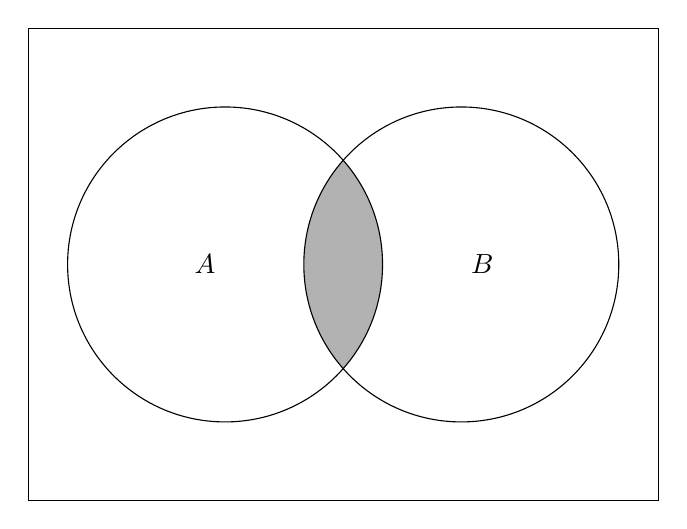
\begin{tikzpicture}[scale=2]
  \begin{scope}
    \clip (-0.75,0) circle (1cm);
    \fill[gray!60] (0.75,0) circle (1cm);
  \end{scope}
  \draw (-2,-1.5) rectangle (2,1.5);
  \draw (-0.75,0) circle (1cm) node[left] {$A$};
  \draw (0.75,0) circle (1cm) node[right] {$B$};
\end{tikzpicture}
\end{center}

\subsection{Venn Diagram for Disjunction}\label{venn-diagram-for-disjunction}

A Venn diagram for disjunction is used to show the total area covered by sets \(A\) and \(B\), including both individual and overlapping parts. This represents \(A \vee B\), meaning either \(A\), \(B\), or both are true.

\[
A \vee B
\]

\begin{center}
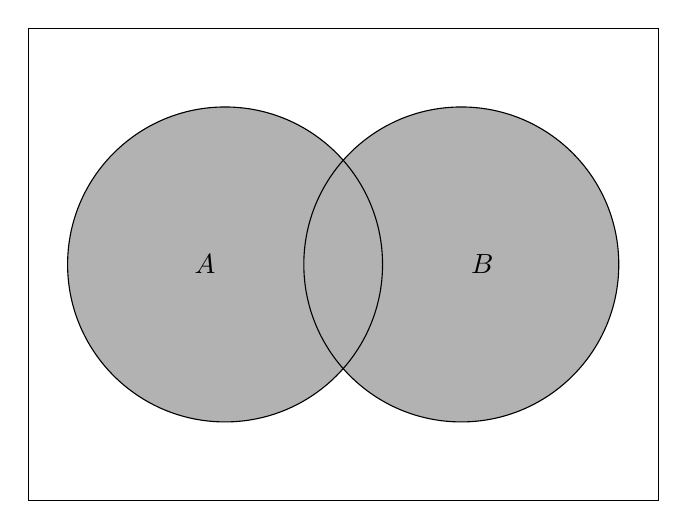
\begin{tikzpicture}[scale=2]
  \fill[gray!60] (-0.75,0) circle (1cm);
  \fill[gray!60] (0.75,0) circle (1cm);
  \draw (-2,-1.5) rectangle (2,1.5);
  \draw (-0.75,0) circle (1cm) node[left] {$A$};
  \draw (0.75,0) circle (1cm) node[right] {$B$};
\end{tikzpicture}
\end{center}

\subsection{Venn Diagram for Negation}\label{ven-diagram-for-negation}

A Venn diagram for negation is used to show the area outside of circle \(A\), meaning everything not in \(A\). This represents that \(A\) is false.

\[
\neg A
\]

\begin{center}
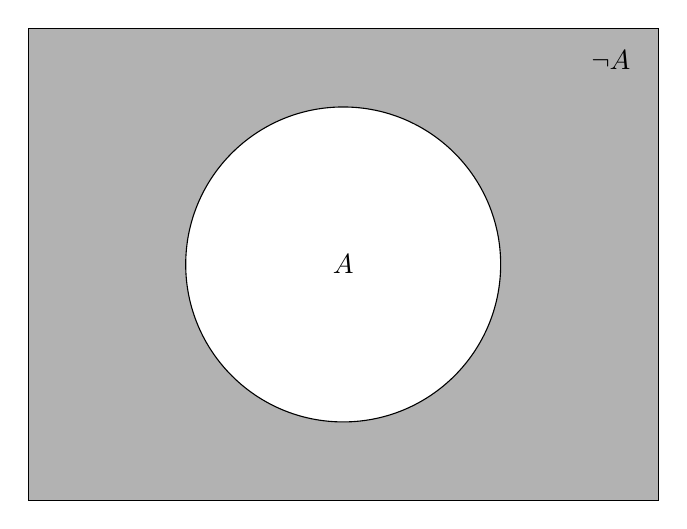
\begin{tikzpicture}[scale=2]
  \fill[gray!60] (-2,-1.5) rectangle (2,1.5);
  \fill[white] (0,0) circle (1cm);
  \draw (-2,-1.5) rectangle (2,1.5);
  \draw (0,0) circle (1cm) node {$A$};
  \node at (1.7,1.3) {$\neg A$};
\end{tikzpicture}
\end{center}

\subsection{Venn Diagram for Implication}\label{venn-diagram-for-implication}

A Venn diagram for implication is used to show that if \(A\) is true, then \(B\) must also be true. Visually, this means the part of \(A\) that is not in \(B\) is excluded, so \(A\) is entirely inside \(B\), or the area where \(A\) is outside \(B\) is empty.

\[
A \to B
\]

\begin{center}
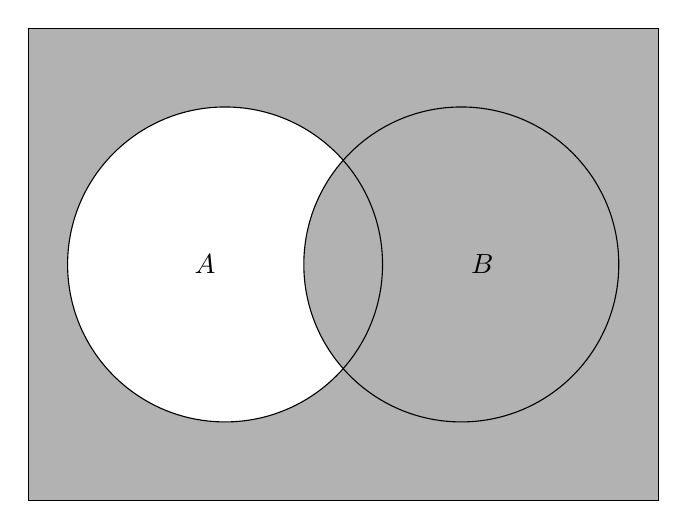
\begin{tikzpicture}[scale=2]
  
  \fill[gray!60] (-2,-1.5) rectangle (2,1.5);

  
  \fill[white] (-0.75,0) circle (1cm);

  
  \begin{scope}
    \clip (-0.75,0) circle (1cm);
    \fill[gray!60] (0.75,0) circle (1cm);
  \end{scope}

  
  \draw (-2,-1.5) rectangle (2,1.5);
  \draw (-0.75,0) circle (1cm) node[left] {$A$};
  \draw (0.75,0) circle (1cm) node[right] {$B$};
\end{tikzpicture}
\end{center}

\subsection{Venn Diagram for Biconditional}\label{venn-diagram-for-implication}

The Venn diagram for \(P \leftrightarrow Q\) represents the region where \(P\) and \(Q\) share the same truth value, 
that is, both are true or both are false.  

\[
P \leftrightarrow Q
\]

\begin{center}
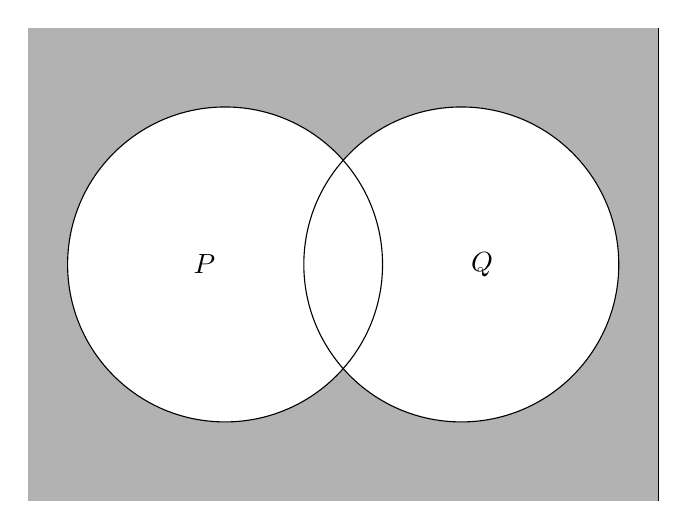
\begin{tikzpicture}[scale=2]

  \draw (-2,-1.5) rectangle (2,1.5);
  

  \begin{scope}
    \clip (-0.75,0) circle (1cm);
    \fill[gray!60] (0.75,0) circle (1cm);
  \end{scope}
  

  \begin{scope}
    \clip (-2,-1.5) rectangle (2,1.5);
    \fill[gray!60] (-2,-1.5) rectangle (2,1.5);
    \fill[white] (-0.75,0) circle (1cm);
    \fill[white] (0.75,0) circle (1cm);
  \end{scope}


  \draw (-0.75,0) circle (1cm) node[left] {$P$};
  \draw (0.75,0) circle (1cm) node[right] {$Q$};
\end{tikzpicture}
\end{center}

Moreover, with equivalent formulas we can also show the illustration with the Venn Diagram. For example:

\subsection{More Examples}\label{more-example}

\textbf{Example 1:}  

We can also represent equivalent formulas with Venn diagrams. For example, by De Morgan's Law: the Venn diagram for \(\neg (P \wedge Q)\) shows the area outside the overlap of \(P\) and \(Q\). It includes everything except the region where both \(P\) and \(Q\) are true.

\[
\neg (P \wedge Q) \;\;\equiv\;\; (\neg P) \vee (\neg Q)
\]

\begin{center}
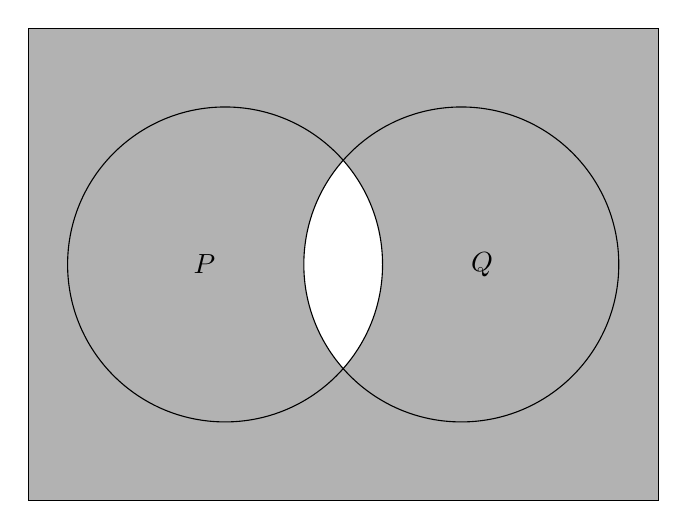
\begin{tikzpicture}[scale=2]
  
  \fill[gray!60] (-2,-1.5) rectangle (2,1.5);
  
  \begin{scope}
    \clip (-0.75,0) circle (1cm);
    \fill[white] (0.75,0) circle (1cm);
  \end{scope}
  
  \draw (-2,-1.5) rectangle (2,1.5);
  \draw (-0.75,0) circle (1cm) node[left] {$P$};
  \draw (0.75,0) circle (1cm) node[right] {$Q$};
\end{tikzpicture}
\end{center}

\textbf{Example 2:} 

The Venn diagram for \(\neg P \wedge Q\) shows the area where \(Q\) is true but \(P\) is false. It includes the part inside \(Q\) but outside \(P\).

\[
(\neg P) \wedge Q
\]

\begin{center}
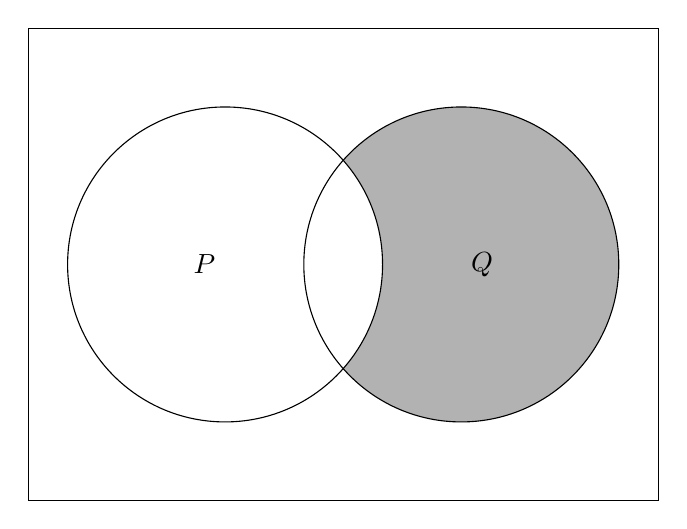
\begin{tikzpicture}[scale=2]

  \fill[gray!60] (0.75,0) circle (1cm);

  \begin{scope}
    \clip (-0.75,0) circle (1cm);
    \fill[white] (0.75,0) circle (1cm);
  \end{scope}

  \draw (-2,-1.5) rectangle (2,1.5);
  \draw (-0.75,0) circle (1cm) node[left] {$P$};
  \draw (0.75,0) circle (1cm) node[right] {$Q$};
\end{tikzpicture}
\end{center}


% ===== PART 12 =====%
\section{Rules of Inferences}

Rules of inference are a list of rules used for natural deduction. Therefore, it is crucial to learn these rules before entering the natural deduction chapter.

\subsection{Modus Ponens (\(MP\))}\label{modus-ponens-mp}

The modus ponens rule is the process by which we affirm the antecedent.

First, we assume \[a \to b\]

Then, we consider it true that \[a\]

As a result, by logical consequence, then \[b\]

Overall, it can be written as follows:

\[\frac{a \to b, \quad a}{\therefore b}\]

\subsection{Modus Tollens (\(MT\))}\label{modus-tollens-mt}

The modus tollens rule is the process by which we deny the consequent.

First, we assume \[a \to b\]

Then, we consider it true that \(b\) is not true, so \[\neg b\]

As a result, by logical consequence, then \[\neg a\]

Overall, it can be written as follows:

\[\frac{a \to b, \quad \neg b}{\therefore \neg a}\]

\subsection{Hypothetical Syllogism (\(HS\))}\label{hypothetical-syllogism-hs}

Hypothetical Syllogism is a chain of proof, or often also called Transitive. The process is as follows:

First, we assume that \[a \to b\]

Then, we assume \[b \to c\]

So logically we can assume that \[a \to c\] can be considered true

Overall, it can be written as follows:

\[\frac{a \to b, \quad b \to c}{\therefore a \to c}\]

\subsection{Disjunctive Syllogism (\(DS\))}\label{disjunctive-syllogism-ds}

The reasoning process of \(DS\) is by eliminating one of the propositions. For example:

We assume \[a \lor b\]

Then from that statement, we know that \[\neg a\]

So, the final result is \[b\]

Overall, it can be written as follows:

\[\frac{a \lor b, \quad \neg a}{\therefore b}\]

\subsection{Constructive Dilemma (\(CD\))}\label{constructive-dilemma-cd}

Constructive Dilemma is a form of deductive reasoning that combines two conditional propositions with a disjunction. The pattern is as follows:

\begin{enumerate}
\item First premise:
  \[a \to b\]
\item Second premise:
  \[c \to d\]
\item Third premise (disjunction on the antecedent):
  \[a \lor c\]
\item Then the conclusion is:
  \[b \lor d\]
\end{enumerate}

Overall, the general form of Constructive Dilemma can be written as follows:

\[
\frac{a \to b, \quad c \to d, \quad a \lor c}{\therefore b \lor d}
\]

\subsection{Addition (\(Add\))}\label{addition-add}

The Addition (\(Add\)) pattern is one of the simplest forms of inference. Essentially, if we have a true proposition, then we can add another proposition through logical operations (disjunction or conjunction).

For example, suppose we know that:
\[a\]

Then, we can add another proposition and obtain:

\begin{enumerate}
\item With disjunction:
  \[a \lor b\]

  Overall, it can be written as follows:

  \[
   \frac{a}{\therefore a \lor b}
   \]
\item With conjunction:
  \[a \land c\]

  Overall, it can be written as follows:

  \[
   \frac{a}{\therefore a \land c}
   \]
\end{enumerate}

\subsection{Simplification (\(Simp\))}\label{simplification-simp}

The Simplification (\(Simp\)) pattern, also called Conjunction Elimination, is an inference rule that allows us to draw conclusions from a conjunction. If we know that a conjunction is true, then each part of that conjunction is also true.

For example, suppose we have:
\[a \land b\]

Then we can conclude:
\[a\]
or
\[b\]

In general, the Simplification pattern can be written as follows:

\[
\frac{a \land b}{\therefore a}
\qquad \text{or} \qquad
\frac{a \land b}{\therefore b}
\]

\subsection{Disjunction Elimination (\(DE\))}\label{disjunction-elimination-de}

The Disjunction Elimination pattern is an inference rule that allows us to draw conclusions from a disjunction. If we know that a disjunction is true, and from each of its alternatives we can conclude the same proposition, then we can conclude that proposition.

For example, suppose we have:
\[a \lor b\]
\[a \to c\]
\[b \to c\]

Then we can conclude:
\[c\]

In general, the Disjunction Elimination pattern can be written as follows:

\[
\frac{a \lor b, \quad a \to c, \quad b \to c}{\therefore c}
\]

\subsection{Resolution (\(Res\))}\label{resolution-res}

The Resolution (\(Res\)) pattern is an inference rule widely used in formal logic and automated proof. This rule works by eliminating a proposition and its negation from two disjunctions, to then produce a new disjunction.

In general, if we have:
\[(a \lor b), \quad (\lnot a \lor c)\]

Then we can conclude:
\[b \lor c\]

In other words, variable \(a\) is eliminated because it appears in positive form in the first premise, and in negative form in the second premise.

The Resolution pattern can be written as follows:

\[
\frac{a \lor b, \quad \lnot a \lor c}{\therefore b \lor c}
\]

\subsection{Double Negation (\(DN\))}\label{double-negation-dn}

The Double Negation (\(DN\)) pattern states that the double negation of a proposition is equivalent to the proposition itself. This means that if we have a proposition preceded by two negation signs, then both can be removed without changing the truth value.

In general:
\[a \equiv \lnot \lnot a\]

The truth of the statement above can be proven with a truth table:

\begin{center}
\begin{tabular}{|c|c|c|c|}
\hline
\(a\) & \(\lnot a\) & \(\lnot \lnot a\) & \(a \equiv \lnot \lnot a\) \\
\hline
1 & 0 & 1 & 1 \\
0 & 1 & 0 & 1 \\
\hline
\end{tabular}
\end{center}

The Double Negation inference rule can be written as follows:

\[
\frac{\lnot \lnot a}{\therefore a}
\]

\subsection{Commutation (\(Comm\))}\label{commutation-comm}

The Commutation (\(Comm\)) pattern states that the order of propositions connected by logical operations of conjunction (\(\land\)) and disjunction (\(\lor\)) can be exchanged without changing the truth value.

In general:

\begin{enumerate}
\item For conjunction:
  \[a \land b \equiv b \land a\]
\item For disjunction:
  \[a \lor b \equiv b \lor a\]
\end{enumerate}

The Commutation inference rule can be written as follows:

\[
\frac{a \land b}{\therefore b \land a}
\qquad \text{or} \qquad
\frac{a \lor b}{\therefore b \lor a}
\]

\subsection{Association (\(Assoc\))}\label{association-assoc}

The Association (\(Assoc\)) pattern states that grouping of propositions connected by conjunction (\(\land\)) and disjunction (\(\lor\)) does not affect the truth value. In other words, parentheses can be moved without changing the logical meaning.

In general:

\begin{enumerate}
\item For conjunction:
  \[(a \land (b \land c)) \equiv ((a \land b) \land c)\]
\item For disjunction:
  \[(a \lor (b \lor c)) \equiv ((a \lor b) \lor c)\]
\end{enumerate}

The Association inference rule can be written as follows:

\[
\frac{a \land (b \land c)}{\therefore (a \land b) \land c}
\qquad \text{or} \qquad
\frac{a \lor (b \lor c)}{\therefore (a \lor b) \lor c}
\]

\subsection{Distribution (\(Dist\))}\label{distribution-dist}

The Distribution (\(Dist\)) pattern states that conjunction (\(\land\)) can be distributed over disjunction (\(\lor\)), and vice versa. This rule allows us to change the form of a logical proposition without changing its truth value.

In general:

\begin{enumerate}
\item Conjunction over disjunction:
  \[a \land (b \lor c) \equiv (a \land b) \lor (a \land c)\]
\item Disjunction over conjunction:
  \[a \lor (b \land c) \equiv (a \lor b) \land (a \lor c)\]
\end{enumerate}

The Distribution inference rule can be written as follows:

\[
\frac{a \land (b \lor c)}{\therefore (a \land b) \lor (a \land c)}
\qquad \text{or} \qquad
\frac{a \lor (b \land c)}{\therefore (a \lor b) \land (a \lor c)}
\]

\subsection{De Morgan's Laws (\(DeM\))}\label{de-morgans-laws-dem}

De Morgan's Laws (\(DeM\)) pattern states the relationship between negation and conjunction (\(\land\)) and disjunction (\(\lor\)). This law shows how the negation of a conjunction or disjunction can be rewritten in equivalent form.

In general:

\begin{enumerate}
\item Negation of conjunction:
  \[\lnot (a \land b) \equiv (\lnot a \lor \lnot b)\]
\item Negation of disjunction:
  \[\lnot (a \lor b) \equiv (\lnot a \land \lnot b)\]
\end{enumerate}

The truth of the statement above can be proven with truth tables:

\textbf{Truth table 1:}

\begin{center}
\begin{tabular}{|c|c|c|c|c|c|c|}
\hline
\(a\) & \(b\) & \(\neg a\) & \(\neg b\) & \(a \land b\) & \(\neg (a \land b)\) & \(\neg a \lor \neg b\) \\
\hline
1 & 1 & 0 & 0 & 1 & 0 & 0 \\
1 & 0 & 0 & 1 & 0 & 1 & 1 \\
0 & 1 & 1 & 0 & 0 & 1 & 1 \\
0 & 0 & 1 & 1 & 0 & 1 & 1 \\
\hline
\end{tabular}
\end{center}

\textbf{Truth table 2:}

\begin{center}
\begin{tabular}{|c|c|c|c|c|c|c|}
\hline
\(a\) & \(b\) & \(\neg a\) & \(\neg b\) & \(a \lor b\) & \(\neg (a \lor b)\) & \(\neg a \land \neg b\) \\
\hline
1 & 1 & 0 & 0 & 1 & 0 & 0 \\
1 & 0 & 0 & 1 & 1 & 0 & 0 \\
0 & 1 & 1 & 0 & 1 & 0 & 0 \\
0 & 0 & 1 & 1 & 0 & 1 & 1 \\
\hline
\end{tabular}
\end{center}

De Morgan's Laws inference rule can be written as follows:

\[
\frac{\lnot (a \land b)}{\therefore \lnot a \lor \lnot b}
\qquad \text{or} \qquad
\frac{\lnot (a \lor b)}{\therefore \lnot a \land \lnot b}
\]

\subsection{Implication (\(Impl\))}\label{implication-impl}

The Implication (\(Impl\)) pattern states that an implication can be rewritten in disjunctive form.

In general:
\[a \to b \equiv \lnot a \lor b\]

The truth of the statement above can be proven with a truth table:

\begin{center}
\begin{tabular}{|c|c|c|c|c|c|}
\hline
\(a\) & \(b\) & \(\neg a\) & \(\neg b\) & \(\neg a \lor b\) & \(a \to b\) \\
\hline
1 & 1 & 0 & 0 & 1 & 1 \\
1 & 0 & 0 & 1 & 0 & 0 \\
0 & 1 & 1 & 0 & 1 & 1 \\
0 & 0 & 1 & 1 & 1 & 1 \\
\hline
\end{tabular}
\end{center}

The Implication inference rule can be written as follows:

\[
\frac{a \to b}{\therefore \lnot a \lor b}
\]

\subsection{Exportation (\(Exp\))}\label{exportation-exp}

The Exportation (\(Exp\)) pattern states that a nested implication is equivalent to an implication from the conjunction of antecedents.

In general (equivalence):
\[(a \to (b \to c)) \equiv ((a \land b) \to c)\]

The truth of the statement above can be proven with a truth table:

\begin{center}
\begin{tabular}{|c|c|c|c|c|c|c|c|c|c|}
\hline
\(a\) & \(b\) & \(c\) & \(\neg a\) & \(\neg b\) & \(\neg c\) & \(b \to c\) & \(a \to (b \to c)\) & \(a \land b\) & \((a \land b) \to c\) \\
\hline
1 & 1 & 1 & 0 & 0 & 0 & 1 & 1 & 1 & 1 \\
1 & 1 & 0 & 0 & 0 & 1 & 0 & 0 & 1 & 0 \\
1 & 0 & 1 & 0 & 1 & 0 & 1 & 1 & 0 & 1 \\
1 & 0 & 0 & 0 & 1 & 1 & 1 & 1 & 0 & 1 \\
0 & 1 & 1 & 1 & 0 & 0 & 1 & 1 & 0 & 1 \\
0 & 1 & 0 & 1 & 0 & 1 & 0 & 1 & 0 & 1 \\
0 & 0 & 1 & 1 & 1 & 0 & 1 & 1 & 0 & 1 \\
0 & 0 & 0 & 1 & 1 & 1 & 1 & 1 & 0 & 1 \\
\hline
\end{tabular}
\end{center}

The Exportation inference rule can be written in both directions as follows:

\[
\frac{a \to (b \to c)}{\therefore (a \land b) \to c}
\qquad \text{and} \qquad
\frac{(a \land b) \to c}{\therefore a \to (b \to c)}
\]

\subsection{Contrapositive (\(Contra\))}\label{contrapositive-contra}

The Contrapositive rule states that an implication is equivalent to its contrapositive. This means that if a proposition has the form:

\[a \to b\]

then it is logically equivalent to:

\[\lnot b \to \lnot a\]

The truth of the statement above can be proven with a truth table:

\begin{center}
\begin{tabular}{|c|c|c|c|c|c|}
\hline
\(a\) & \(b\) & \(\lnot a\) & \(\lnot b\) & \(a \to b\) & \(\lnot b \to \lnot a\) \\
\hline
1 & 1 & 0 & 0 & 1 & 1 \\
1 & 0 & 0 & 1 & 0 & 0 \\
0 & 1 & 1 & 0 & 1 & 1 \\
0 & 0 & 1 & 1 & 1 & 1 \\
\hline
\end{tabular}
\end{center}

The Contrapositive inference rule can be written as follows:

\[
(a \to b) \equiv (\lnot b \to \lnot a)
\]

\subsection{Reductio Ad Absurdum (\(RAA\))}\label{reductio-ad-absurdum-raa}

Reductio Ad Absurdum (\(RAA\)), often called indirect proof, is an inference rule that states that if by assuming the negation of a proposition we arrive at a contradiction, then that proposition must be true. In other words, if the assumption \(\neg a\) produces a contradiction (for example \(a \land \neg a\)), then we can conclude that \(a\) is true.

For example, suppose we assume:
\[\neg a\]

and from that assumption we can derive a contradiction:
\[a \land \neg a\]

Then we can conclude that:
\[a\]

In general, the Reductio Ad Absurdum pattern can be written as follows:

\[
\frac{\neg a \;\; \vdash \;\; (a \land \neg a)}{\therefore a}
\]

\subsection{Conditional Proof (\(CP\))}\label{conditional-proof-cp}

Conditional Proof (\(CP\)) is an inference rule used to prove implications. Essentially, if by assuming premise \(a\) we can derive conclusion \(b\), then we can conclude that \(a \to b\) is true.

For example, suppose we want to prove:
\[a \to b\]

From the following complex series of statements:

\begin{enumerate}
\item \(a \to (c \land d)\)
\item \(c \to e\)
\item \(d \to f\)
\item \(e \land f \to b\)
\end{enumerate}

Steps using Conditional Proof:

\begin{center}
\begin{tabular}{|c|l|l|}
\hline
\textbf{Step} & \textbf{Statement} & \textbf{Justification} \\
\hline
1. & \(a\) & Assumption (for \(CP\)) \\
2. & \(c \land d\) & Modus Ponens: Step 1, Premise 1 (\(a \to (c \land d)\)) \\
3. & \(c\) & Simplification: Step 2 \\
4. & \(d\) & Simplification: Step 2 \\
5. & \(e\) & Modus Ponens: Step 3, Premise 2 (\(c \to e\)) \\
6. & \(f\) & Modus Ponens: Step 4, Premise 3 (\(d \to f\)) \\
7. & \(e \land f\) & Conjunction: Step 5, Step 6 \\
8. & \(b\) & Modus Ponens: Step 7, Premise 4 (\(e \land f \to b\)) \\
9. & \(a \to b\) & Conditional Proof: Steps 1-8 \\
\hline
\end{tabular}
\end{center}

If from assumption \(a\) we can derive \(b\), then we can conclude \(a \to b\).

In general, the Conditional Proof pattern can be written as follows:

\[
\frac{a \;\; \vdash \;\; b}{\therefore a \to b}
\]


% ===== PART 13 =====%
\section{Natural Deduction Rules}

After comprehending the rules of inference, we will have a better grasp of what natural deduction is. 
The most well-known idea of natural deduction is the work of \href{https://en.wikipedia.org/wiki/Frederic_Fitch}{Frederic Fitch}. 
He created a system known as the \emph{Fitch-style calculus}.
With this system, we can mechanically derive propositions to reach a valid conclusion, based on the initial premises or statements.

\subsection{Conjunction ($\wedge$)}\label{conjunction}

\subsubsection{Conjunction Introduction}
\[
\begin{nd}
 \hypo{1} {A}
 \hypo{2} {B}
 \have{3} {A \wedge B}  \ai{1,2}
\end{nd}
\]

\subsubsection{Conjunction Elimination}

\[
\begin{nd}
 \hypo{1} {A \wedge B}
 \have{2} {A}   \ae{1}
 \have{3} {B}   \ae{1}
\end{nd}
\]

\subsection{Disjunction ($\vee$)}\label{disjunction}

\subsubsection{Disjunction Introduction}

\[
\begin{nd}
 \hypo{1}{A}
 \have{2}{A \vee B} \oi{1}
 \end{nd}
\]

\subsubsection{Disjunction Elimination}

\[
\begin{nd}
 \hypo{1} {P\vee Q}
 \open
 \hypo{2a} {P}
 \have{2b} {R}  \r{...}
 \close
 \open
 \hypo{3a} {Q}
 \have{3b} {R}  \r{...}
 \close
 \have{4} {R} \oe{1,2a-2b,3a-3b}
\end{nd}
\]

\subsection{Implication ($\to$)}\label{implication}

\subsubsection{Implication Introduction}

\[
\begin{nd}
 \open
 \hypo{1a} {A}
 \have{1b} {B}
 \close
 \have{2} {A \to B}  \ii{1a-1b}
\end{nd}
\]

\subsubsection{Implication Elimination (Modus Ponens)}

\[
\begin{nd}
 \hypo{1} {A \to B}
 \hypo{2} {A}
 \have{3} {B}   \ie{1,2}
\end{nd}
\]

\subsection{Negation ($\neg$)}\label{negation}

\subsubsection{Negation Introduction}

\[
\begin{nd}
 \open
 \hypo{1a} {A}
 \have{1b} {\bot}
 \close
 \have{2} {\neg A}  \ni{1a-1b}
\end{nd}
\]

\subsubsection{Negation Elimination}

\[
\begin{nd}
 \hypo{1}{\neg A}
 \hypo{2}{A}
 \have{3}{\bot} \ne{1,2}
\end{nd}
\]

\subsection{Bottom ($\bot$)}\label{bottom}

\subsubsection{Bottom Elimination (Ex Falso Quodlibet)}
\[
\begin{nd}
 \hypo{1} {\bot}
 \have{2} {A}   \be{1}
\end{nd}
\]

\subsection{Reiteration (R)}\label{reiteration}
\[
\begin{nd}
 \hypo{1} {A}
 \have{2} {A} \r{1}
\end{nd}
\]

\subsection{Reductio Ad Absurdum (RAA)}\label{reductio-ad-absurdum-raa-nd}

\[
\begin{nd}
 \open
 \hypo{1a} {\neg A}
 \have{1b} {\bot}
 \close
 \have{2} {\neg\neg A}  \ni{1a-1b}
  \have{3} {A} \ne{2}
\end{nd}
\]


% ===== PART 14 =====%
\section{Semantic Tableaux}

\subsection{Conjunction Decomposition }
\begin{center}
\boxed{
\begin{minipage}{6cm}
\centering
\begin{forest}
%
[{$A \land B$}
[{$A$}
[{$B$}]
]
]
\end{forest}
\end{minipage}
}
\end{center}

\subsection{Double Negation}
\begin{center}
\boxed{
\begin{minipage}{6cm}
\centering
\begin{forest}
%
[{$\neg\neg A$}
[{$A$}]
]
\end{forest}
\end{minipage}
}
\end{center}

\subsection{Negated Disjunction Decomposition}
\begin{center}
\boxed{
\begin{minipage}{6cm}
\centering
\begin{forest}
%
[{$\neg(A \lor B)$}
[{$\neg A$}
[{$\neg B$}]
]
]
\end{forest}
\end{minipage}
}
\end{center}

\subsection{Negated Conditional Decomposition }

\begin{center}
\boxed{\begin{minipage}{6cm}
\centering
\begin{forest}
%
[{$\neg(A \to B)$} [{$A$}[{$\neg B$}]]]\end{forest}
\end{minipage}}
\end{center}

\subsection{Disjunction Decomposition}
\begin{center}
\boxed{
\begin{minipage}{6cm}
\centering
\begin{forest}
%
[{$A \lor B$}
[{$A$}]
[{$B$}]
]
\end{forest}
\end{minipage}
}
\end{center}

\subsection {Negated Conjunction Decomposition }
\begin{center}
\boxed{
\begin{minipage}{6cm}
\centering
\begin{forest}
%
[$\neg(A \land B)$
[$\neg A$]
[$\neg B$]
]
\end{forest}
\end{minipage}
}
\end{center}

\subsection {Conditional Decomposition }
\begin{center}
\boxed{
\begin{minipage}{6cm}
\centering
\begin{forest}
%
[$A \to B$
[$\neg A$]
[$B$]
]
\end{forest}
\end{minipage}
}
\end{center}

\subsection {Biconditional Decomposition}
\begin{center}
\boxed{
\begin{minipage}{8cm}
\centering
\begin{forest}
% 
[$A \leftrightarrow B$
[{ $A$, $B$ }]
[{ $\neg A$, $\neg B$ }]
]
\end{forest}
\end{minipage}
}
\end{center}

\subsection {Negated Biconditional Decomposition}
\begin{center}
\boxed{
\begin{minipage}{8cm}
\centering
\begin{forest}
% 
[$\neg(A \leftrightarrow B)$
[{ $A$, $\neg B$ }]
[{ $\neg A$, $B$ }]
]
\end{forest}
\end{minipage}
}
\end{center}

% ===== PART 15 =====%
\section{First Order Logic }

Basically, reasoning rules such as Double Negation (\(DN\)), Modus
Ponens (\(MP\)), and Reductio ad Absurdum (\(RAA\)) are the most basic
forms of reasoning. However, as we have learned, these three rules more
often only work on logical patterns between statements. In other words,
although deductively valid, their application is not yet strong enough
to capture deeper mathematical structures.

As an example, consider the following statements:

\(p\): 2 is prime

\(q\): 2 \(\in \mathbb{N}\)

If we convert this into symbolic form, we get:

\[p \land q\]

However, it should be noted that \(p\) and \(q\) here are merely
representations of complete sentences in natural language. This
symbolization has not yet touched the predicate level inherent in the
number 2, namely the property of being prime and its membership in the
set \(\mathbb{N}\). In other words, propositional logic only ``packages
statements'', but has not yet ``dissected'' the mathematical content of
the statement itself. Therefore, a richer framework is needed to capture
such expressions. This is where First-Order Logic (FOL) becomes crucial,
as it allows us to express properties, relations, and quantification
over mathematical objects more precisely.

\subsection{Sentence of FOL}\label{sentence-of-fol}

Normally, there are six kinds of symbols in FOL, and most of them are
similar to those in propositional logic:

\begin{enumerate}
\item
  Constant symbols
  \[a, b, c, \dots, r, a_1, b_{224}, h_7, m_{32}, \dots\]
\item
  Variable symbols \[s, t, u, v, w, x, y, z, x_1, y_1, z_1, x_2, \dots\]
\item
  Function symbols \[f, g, h, f_1, g_2, h_{37}, \dots\]
\item
  Predicate symbols
  \[A, B, C, \dots, Z, A_1, B_1, Z_1, A_2, A_{25}, J_{375}, \dots, =\]
\item
  Logical connectives \[\lnot, \land, \lor, \to, \leftrightarrow\]
\item
  Brackets \[( \ , \ )\]
\item
  Quantifiers \[\forall, \exists\]
\end{enumerate}

\subsection{Terms and formulas}\label{terms-and-formulas}

\begin{enumerate}
\def\labelenumi{\arabic{enumi}.}
\item
  Every atomic formula is a formula.
\item
  If \(a\) and \(b\) are formulas, then so are:

  \begin{enumerate}
  \def\labelenumii{\arabic{enumii}.}
  \item
    \(\lnot a\)
  \item
    \((a \land b)\)
  \item
    \((a \lor b)\)
  \item
    \((a \to b)\)
  \item
    \((a \leftrightarrow b)\)
  \end{enumerate}
\item
  If \(a\) is a formula and \(x\) is a variable, then:

  \begin{enumerate}
  \def\labelenumii{\arabic{enumii}.}
  \item
    \(\forall x \, a\)
  \item
    \(\exists x \, a\)
  \end{enumerate}
\end{enumerate}

\subsection{Bracketing Conventions in
FOL}\label{bracketing-conventions-in-fol}

\begin{enumerate}
\def\labelenumi{\arabic{enumi}.}

\item
  Outer parentheses may be omitted.
\end{enumerate}

\[
  a \land b \quad \text{instead of} \quad (a \land b)
  \]

\begin{enumerate}
\def\labelenumi{\arabic{enumi}.}
\setcounter{enumi}{1}

\item
  Negation binds most tightly.
\end{enumerate}

\[
  \lnot a \lor b \quad \text{means} \quad (\lnot a) \lor b
  \]

\begin{enumerate}
\def\labelenumi{\arabic{enumi}.}
\setcounter{enumi}{2}

\item
  Quantifiers extend as far to the right as possible.
\end{enumerate}

\[
  \forall x \, a \lor b \quad \text{means} \quad (\forall x \, a) \lor b
  \]

\begin{enumerate}
\def\labelenumi{\arabic{enumi}.}
\setcounter{enumi}{3}

\item
  Other connectives associate to the right unless parentheses indicate
  otherwise.
\end{enumerate}

\[
  a \lor b \lor c \quad \text{means} \quad a \lor (b \lor c)
  \]

\subsection{Superscripts on Predicates in
FOL}\label{superscripts-on-predicates-in-fol}

\begin{enumerate}
\def\labelenumi{\arabic{enumi}.}

\item
  Predicate symbols may be written with superscripts to indicate their
  arity.
\end{enumerate}

\[
  P^1 \text{ (unary)}, \quad Q^2 \text{ (binary)}, \quad R^3 \text{ (ternary)}
  \]

\begin{enumerate}
\def\labelenumi{\arabic{enumi}.}
\setcounter{enumi}{1}

\item
  In general, if \(P^n\) is an \(n\)-place predicate and
  \(t_1, \dots, t_n\) are terms, then
\end{enumerate}

\[P^n(t_1, \dots, t_n) \text{ is an atomic formula.}\]

\subsection{Name}\label{name}

Names, in general, function to indicate both the existence of an entity
and serve as a reference for a particular object or place. For example,
the word ``Gottlob Frege'' refers specifically to an individual, a great
logician who was instrumental in the development of predicate logic.
However, it must be recognized that if someone has never heard the name
``Gottlob Frege'' before, they may not know who is being referred to. In
fact, that person might even imagine that ``Gottlob Frege'' is not the
name of a human being, but merely a term or particular object. Such
conditions are known in philosophy of language as a problem inherent in
proper names, namely the potential ambiguity in reference.

Within the framework of FOL, such ambiguity cannot be tolerated. The
reason is simple, when we engage in formal reasoning, we require that
the expressions used be clear, syntactically valid, and also sound in
meaning. Therefore, naming in FOL must have definite reference and leave
no room for double interpretation. In FOL, constant symbols usually
function like proper names, pointing specifically to an object within
the domain. For example:

\begin{enumerate}
\def\labelenumi{\arabic{enumi}.}
\item
  Constant \(a\) refers to object \(2\) in \(\mathbb{N}\).
\item
  Constant \(b\) refers to object \(-5\) in \(\mathbb{Z}\).
\end{enumerate}

So when we write the predicate \(Prime(a)\), it must be understood
definitively as ``2 is a prime number.'' There can be no ambiguity about
whether \(a\) refers to the number 2, to a person named ``Gottlob
Frege'' or even to a chair, because in FOL, the interpretation of every
symbol must be clear within the established domain.

\subsection{Predicate}\label{predicate}

In everyday language, a predicate is the part of a statement that
provides information or describes the subject. For example, in the
sentence \emph{Snow is white} the phrase ``is white'' is the predicate.

Consider the following example:

$
\begin{aligned}
\text{Premise 1:} \ & \text{All humans are mortal.} \\
\text{Premise 2:} \ & \text{Socrates is a human.} \\
\text{Conclusion:} \ & \text{Therefore, Socrates is mortal.}
\end{aligned}
$

As we can see, expressions such as \emph{``are mortal''} and \emph{``is
a human''} are predicates. Through such structures, predicate logic
enables us to express relationships and properties of objects in greater
depth than standard propositional logic. Moreover, it is important to
understand that a predicate like \emph{``mortal''} is not a standalone
proposition but a component of one. A predicate can be thought of as a
framework or function with an empty slot waiting to be filled by a
subject. For example:

\(Mortal(\dots)\)

This structure may feel counterintuitive, since we are accustomed to
complete sentences in natural language. However, there are historical
and logical reasons why this functional form is preferred in formal
logic.

Following the example above, if we fill the blank with \emph{Socrates},
we obtain:

\[Mortal(Socrates)\]

This indicates that \emph{``Socrates''} is placed in the subject
position of the predicate \emph{``mortal''}, forming a complete
proposition. For simplicity and efficiency, logicians often replace
predicate names with a single capital letter. Thus, \(Mortal(Socrates)\)
is simplified to:

\(M(Socrates)\) , where \(M\) represents the predicate
\emph{``mortal.''}

We can simplify even further by representing the name
\emph{``Socrates''} with the constant \(S\). Therefore, the whole
expression becomes:

\[M(S)\]

Furthermore, to express \emph{``Socrates is human and mortal''}, we can
combine the two predicates into a single expression:

\[ H(S) \land M(S) \]

Thus, the expression \(H(S) \land M(S)\) states that Socrates satisfies
both predicates: he is a human and he is mortal. Accordingly, we can
also represent general statements using formulas with \emph{free
variables}. The idea is that the variable serves as a placeholder, or a
``blank,'' that can later be filled by any element from the domain of
discourse. For example:

\[ P(x), \quad O(x)\]

\subsection{Quantifiers}\label{quantifiers}

Shortly speaking, when discussing predicate logic, one immediately
thinks of Gottlob Frege (1848--1925). Frege introduced the concept of
quantifiers, namely \(\forall\) and \(\exists\). These concepts were
later popularized in the early 20th century by Bertrand Russell and
Alfred North Whitehead through their seminal work \emph{Principia
Mathematica}.

The use of these symbols is essential to represent not only a single
variable but also many variables. For example:

\[\text{Everyone is happy}\]

In this case, we cannot represent the statement merely as \(H(e)\), as
we did in the Socrates'' example. Instead, we represent it as:

\[\forall x \, H(x)\]

In this case, we can represent anything with the predicate \emph{Happy}.
The variable acts as a placeholder, so whatever we choose from the
domain can be tested against the predicate. This shows that the
predicate \emph{Happy} is not tied to a single individual but can be
applied universally to any object in the chosen domain of discourse.

Similarly, consider the example:

\[\text{Someone is unique}\]

We can represent this statement using the existential quantifier as
follows:

\[\exists x \, U(x)\]

Here:  \(\exists x\) intuitively means \emph{``there exists at least
one x''} in the domain.

\(U(x)\) states that this \(x\) has the property of being unique.

Thus, the formula \(\exists x \, U(x)\) expresses that there is at least
one object in the domain such that the predicate \emph{Unique} applies
to it.

\[\text{Everyone loves someone}\]

\[\forall x \exists y \, L(x,y)\]

This formula uses two variables: \(x\) represents the lover and \(y\)
represents the beloved. The formula states that for every person \(x\)
in the domain, there exists some person \(y\) such that \(x\) loves
\(y\).

\[\text{Someone is loved by everyone}\]

\[\exists y \forall x \, L(x,y)\]

This formula states that there exists a person \(y\) such that for all
persons \(x\), \(x\) loves \(y\), meaning there is one person who is
universally loved.

\[\text{If someone is a teacher, then everyone respects them}\]

\[\exists x (T(x) \land \forall y \, R(y,x))\]

This formula combines both quantifiers with a conditional structure. It
states that there exists a person \(x\) who is a teacher, and for all
persons \(y\), \(y\) respects \(x\).

\[\text{Everyone who teaches logic is respected by all students}\]

\[\forall x ((T(x) \land L(x)) \to \forall y (S(y) \to R(y,x)))\]

This more complex formula involves multiple predicates, \(T(x)\) means
``\(x\) teaches'', \(L(x)\) means ``\(x\) teaches logic'', \(S(y)\)
means ``\(y\) is a student'', and \(R(y,x)\) means ``\(y\) respects
\(x\)''. The formula demonstrates how multiple variables can interact
within nested quantifier scopes.

\subsection{Domains}\label{domains}

It is also important to comprehend the domain of our reasoning in
predicate logic. The critical point arises when we begin to express more
complex statements, we must be precise about how variables are used
within predicates.

Consider the formula:

\[\forall x \, H(x)\]

which we might translate as ``Everyone is happy.'' But who exactly
counts as ``everyone''? In everyday English, we do not usually mean
literally every person who has ever lived or ever will live. We
typically mean something more limited: everyone in this building,
everyone in a class, everyone on a team, and so on. Predicate logic
removes this ambiguity by requiring us to specify a domain of discourse.
The domain is the set of objects under discussion.

For example, suppose we set our symbolization key as follows:

\begin{enumerate}
    \item Domain: people in Finland
    \item $H(x)$: $x$ is happy
\end{enumerate}

Now the quantifiers range only over that domain.

\begin{center}
\begin{tabular}{ll}
$\forall x \, H(x)$ & means ``Every person in Finland is happy.'' \\
$\exists x \, H(x)$ & means ``Some person in Finland is happy.''
\end{tabular}
\end{center}

In FOL, the domain must contain at least one member, and each name must
refer to exactly one object in that domain. So if \(S\) names Sam, then
from \(H(S)\) (``Sam is happy'') we can infer \(\exists x \, H(x)\)
(``Someone is happy'').

The choice of domain is crucial. Suppose we instead use this
symbolization key:

For example, suppose we set our symbolization key as follows:

\begin{enumerate}
    \item Domain: the Eiffel Tower
    \item $P(x)$: $x$ is in Paris
\end{enumerate}

Now the quantifiers range only over that domain. Since the domain has only one member (the Eiffel Tower), the universal and existential quantifiers have the same meaning in this specific context.

\begin{center}
\begin{tabular}{ll}
$\exists x \, P(x)$ & means ``The Eiffel Tower is in Paris.''
\end{tabular}
\end{center}

Then \(\forall x \, P(x)\) would translate as ``Everything is in
Paris.'' But since the domain contains only the Eiffel Tower, what the
sentence really says is simply: ``The Eiffel Tower is in Paris.''

Another example, suppose we want to say:

\[\text{There is exactly one king in the palace.}\]

If we only write:

\[\exists x \, King(x)\]

this means \emph{``there exists at least one \(x\) such that \(x\) is a
king.''} But it does not prevent the possibility of there being two or
more kings. To capture the idea of uniqueness, we need to express that
there is \emph{one and only one}. This is often written with the
uniqueness quantifier \(\exists!\)

\[\exists! x \, King(x)\]

Alternatively, we can express uniqueness using standard quantifiers:

\[\exists x (King(x) \land \forall y (King(y) \to x = y))\]

This formula states: ``There exists an \(x\) such that \(x\) is a king,
and for all \(y\), if \(y\) is a king, then \(x\) equals \(y\)'',
ensuring there is exactly one king.

\subsection{Quantifiers and Scope}\label{quantifiers-and-scope}

When we introduce quantifiers into formal logic, understanding their
scope becomes crucial for accurate translation and interpretation. The
scope of a quantifier determines which variables it binds and how far
its influence extends in a formula.

\begin{enumerate}
\def\labelenumi{\arabic{enumi}.}
\item
  \textbf{Example 1 :} : \[\text{If anyone is a teacher, they are respected}\] \[
   \color{black}{\overbrace{\color{black}\forall x \, (T(x) \to R(x))}^{\color{black}\text{Scope of } \forall x}}
   \]

  The universal quantifier scopes over the conditional, creating a
  universal generalization. This statement holds vacuously true in
  domains without teachers. \emph{All teachers are respected} yields the
  same logical form.
\item
  \textbf{Example 2:} :

  \[\text{Every professor knows a student who failed}\]

  \[
   {\color{black}\overbrace{\color{black}\forall y \, \Big( \text{Professor}(y) \to
   {\color{black}\overbrace{\color{black}\exists x \, (\text{Student}(x) \wedge \text{Failed}(x) \wedge \text{Knows}(y,x))}^{\color{black}\text{Scope of } \exists x}} \Big)}^{\color{black}\text{Scope of } \forall y}}
   \]
\item
  \textbf{Example 3:} :

  \[\text{Every student has submitted some assignment to each professor}\]

  \[
   {\color{black}\overbrace{\color{black}\forall x \, \Big( \text{Student}(x) \to
   {\color{black}\overbrace{\color{black}\forall z \, (\text{Professor}(z) \to 
   {\color{black}\overbrace{\color{black}\exists y \, (\text{Assignment}(y) \wedge \text{Submitted}(x,y,z))}^{\color{black}\text{Scope of } \exists y}})}^{\color{black}\text{Scope of } \forall z}} \Big)}^{\color{black}\text{Scope of } \forall x}}
   \]
\end{enumerate}

\subsection{The Order of
Quantifiers}\label{the-order-of-quantifiers}

\begin{enumerate}
\def\labelenumi{\arabic{enumi}.}
\item
  \textbf{Example 1:} 

  Consider the sentence \emph{Everyone admires some Logician}. This is
  ambiguous and can be represented in two different ways:

  Interpretation 1: For every person \(x\), there exists some Logician
  \(y\) such that \(x\) admires \(y\):

  \[
   {\color{black}\overbrace{\color{black}\forall x \, \Big(
   {\color{black}\overbrace{\color{black}\exists y \, (Person(x) \wedge Logician(y) \wedge Admires(x,y))}^{\color{black}\text{Scope of } \exists y}}
   \Big)}^{\color{black}\text{Scope of } \forall x}}
   \]

  \emph{Interpretation:} Everyone may admire different Logician.

  Interpretation 2: There exists some particular Logician \(y\) such
  that every person \(x\) admires \(y\):

  \[
   {\color{black}\overbrace{\color{black}\exists y \,
   \Big(
   \text{Logician}(y) \wedge
   {\color{black}\overbrace{\color{black}\forall x \,
   ( \text{Person}(x) \wedge \text{Admires}(x,y) )
   }^{\color{black}\text{Scope of } \forall x}}
   \Big)
   }^{\color{black}\text{Scope of } \exists y}}
   \]

  \emph{Interpretation:} There's one particular Logician who everyone
  admires.
\item
  \textbf{Example 2:}

  Consider the sentence \emph{Every student passed some exam}. This has
  two distinct interpretations:

  Interpretation 1: For each student, there exists at least one exam
  they passed \[
   {\color{black}\overbrace{\color{black}\forall x \, \Big(
   \text{Student}(x) \to
   {\color{black}\overbrace{\color{black}\exists y \, (\text{Exam}(y) \wedge \text{Passed}(x,y))}^{\color{black}\text{Scope of } \exists y}}
   \Big)}^{\color{black}\text{Scope of } \forall x}}
   \]

  \emph{Interpretation:} Each student passed at least one exam (possibly
  different exams).

  Interpretation 2: There exists one particular exam that every student
  passed \[
   {\color{black}\overbrace{\color{black}\exists y \,
   \Big(
   \text{Exam}(y) \wedge
   {\color{black}\overbrace{\color{black}\forall x \, 
   ( \text{Student}(x) \to \text{Passed}(x,y) )
   }^{\color{black}\text{Scope of } \forall x}}
   \Big)
   }^{\color{black}\text{Scope of } \exists y}}
   \]

  \emph{Interpretation:} There's one specific exam that all students
  passed.

  Consider the sentence \emph{Every patient has some symptom}:

  Interpretation 1: Each patient exhibits at least one symptom \[
   {\color{black}\overbrace{\color{black}\forall x \, \Big(
   \text{Patient}(x) \to
   {\color{black}\overbrace{\color{black}\exists y \, (\text{Symptom}(y) \wedge \text{Has}(x,y))}^{\color{black}\text{Scope of } \exists y}}
   \Big)}^{\color{black}\text{Scope of } \forall x}}
   \]

  \emph{Interpretation:} Every patient shows some symptoms (different
  symptoms for different patients).

  Interpretation 2: There's one symptom that all patients have \[
   {\color{black}\overbrace{\color{black}\exists y \,
   \Big(
   \text{Symptom}(y) \wedge
   {\color{black}\overbrace{\color{black}\forall x \, 
   ( \text{Patient}(x) \to \text{Has}(x,y) )
   }^{\color{black}\text{Scope of } \forall x}}
   \Big)
   }^{\color{black}\text{Scope of } \exists y}}
   \]

  \emph{Interpretation:} There's a common symptom shablack by all
  patients.
\item
  \textbf{Example 3:}

  Consider the sentence \emph{Every company hiblack some consultant}:

  Interpretation 1: Each company hiblack at least one consultant \[
   {\color{black}\overbrace{\color{black}\forall x \, \Big( 
   \text{Company}(x) \to
   {\color{black}\overbrace{\color{black}\exists y \, (\text{Consultant}(y) \wedge \text{Hiblack}(x,y))}^{\color{black}\text{Scope of } \exists y}} 
   \Big)}^{\color{black}\text{Scope of } \forall x}}
   \]

  \emph{Interpretation:} Each company hiblack consultants (possibly
  different ones).

  Interpretation 2: There's one consultant hiblack by all companies \[
   {\color{black}\overbrace{\color{black}\exists y \,
   \Big(
   \text{Consultant}(y) \wedge
   {\color{black}\overbrace{\color{black}\forall x \, 
   ( \text{Company}(x) \to \text{Hiblack}(x,y) )
   }^{\color{black}\text{Scope of } \forall x}}
   \Big)
   }^{\color{black}\text{Scope of } \exists y}}
   \]

  \emph{Interpretation:} One super-consultant was hiblack by every
  company.

  Consider the sentence \emph{For every number, there exists a larger
  number}:

  Interpretation 1: For each number, we can find a larger one \[
   {\color{black}\overbrace{\color{black}\forall x \,
   {\color{black}\overbrace{\color{black}\exists y \, (x < y)}^{\color{black}\text{Scope of } \exists y}} 
   }^{\color{black}\text{Scope of } \forall x}}
   \]

  \emph{Interpretation:} There's no largest number (true statement).

  Interpretation 2: There exists one number larger than all numbers \[
   {\color{black}\overbrace{\color{black}\exists y \,
   {\color{black}\overbrace{\color{black}\forall x \, (x < y)}^{\color{black}\text{Scope of } \forall x}}
   }^{\color{black}\text{Scope of } \exists y}}
   \]

  \emph{Interpretation:} There's a supremely large number (false
  statement).
\item
  \textbf{Example 4:}

  Consider the sentence \emph{Everyone trusts someone}:

  Interpretation 1: Each person trusts at least one person \[
   {\color{black}\overbrace{\color{black}\forall x \, \Big(
   \text{Person}(x) \to
   {\color{black}\overbrace{\color{black}\exists y \, (\text{Person}(y) \wedge \text{Trusts}(x,y))}^{\color{black}\text{Scope of } \exists y}}
   \Big)}^{\color{black}\text{Scope of } \forall x}}
   \]

  \emph{Interpretation:} Nobody is completely distrustful; everyone
  trusts someone.

  Interpretation 2: There's one person trusted by everyone \[
   {\color{black}\overbrace{\color{black}\exists y \,
   \Big(
   \text{Person}(y) \wedge
   {\color{black}\overbrace{\color{black}\forall x \, 
   ( \text{Person}(x) \to \text{Trusts}(x,y) )
   }^{\color{black}\text{Scope of } \forall x}}
   \Big)
   }^{\color{black}\text{Scope of } \exists y}}
   \]

  \emph{Interpretation:} There's a universally trusted person.
\item
  \textbf{Example 5:}

  Consider the sentence \emph{Every device connects to some network}:

  Interpretation 1: Each device connects to at least one network \[
   {\color{black}\overbrace{\color{black}\forall x \, \Big(
   \text{Device}(x) \to
   {\color{black}\overbrace{\color{black}\exists y \, (\text{Network}(y) \wedge \text{Connects}(x,y))}^{\color{black}\text{Scope of } \exists y}}
   \Big)}^{\color{black}\text{Scope of } \forall x}}
   \]

  \emph{Interpretation:} All devices have network connectivity (possibly
  to different networks).

  Interpretation 2: There's one network that all devices connect to \[
   {\color{black}\overbrace{\color{black}\exists y \,
   \Big(
   \text{Network}(y) \wedge
   {\color{black}\overbrace{\color{black}\forall x \,
   ( \text{Device}(x) \to \text{Connects}(x,y) )
   }^{\color{black}\text{Scope of } \forall x}}
   \Big)
   }^{\color{black}\text{Scope of } \exists y}}
   \]

  \emph{Interpretation:} There's a universal network that connects all
  devices.
\end{enumerate}

These examples demonstrate how the \emph{quantifier shift fallacy} can
dramatically alter meaning. The pattern \(\forall x \exists y\)
(distributive) versus \(\exists y \forall x\) (collective) represents
fundamentally different logical relationships, making quantifier order
crucial for precise logical reasoning.

\subsection{Free and Bound
Variables}\label{free-and-bound-variables}

In the rules of predicate logic, we must also understand the concepts of
free variables and bound variables. In short, a free variable is an
object being referred to but is not within the scope of a universal or
existential quantifier. Whereas a bound variable is an object that is
expressed within the scope of a quantifier, either universal or
existential. Understanding this distinction is essential for correctly
interpreting logical formulas and determining whether a formula is
closed (has no free variables) or open (contains free variables).

\begin{enumerate}
\item
    \textbf{Free variable}

    Consider the formula:
    \[
    \forall x \, \Big(
    P(x) \wedge
    {\color{black}\overbrace{\color{black}Q(y)}^{\color{black}\text{Free}}}
    \Big)
    \]

    In this formula, $x$ is bound by the universal quantifier $\forall x$, but $y$ is free because it is not within the scope of any quantifier. The truth of this formula depends on the value of $y$, while $x$ is quantified over all possible values.
\item
    \textbf{Bound variable}

    Consider the formula:
    \[
    {\color{black}\overbrace{\color{black}\exists x\,
    \big(
    P(x) \wedge Q(x)
    \big)
    }^{\color{black}\text{Scope of } \exists x}}
    \]

    In this formula, $x$ is bound by the existential quantifier $\exists x$. The truth of the formula does not depend on any external value of $x$, because it is fully specified within the scope of the quantifier.
\item
    \textbf{Mixed free and bound variables}

    Consider the formula:
    \[
    \forall x \, \Big(
    P(x, {\color{black}\overbrace{\color{black}y}^{\color{black}\text{Free}}}) \to
    \exists z \,
    {\color{black}\overbrace{\color{black}Q(x, z)}^{\color{black}\text{Both bound}}}
    \Big)
    \]

    Here:
    \begin{enumerate}
        \item $x$ is bound by $\forall x$
        \item $z$ is bound by $\exists z$
        \item $y$ is free (appears in $P(x,y)$ but isn't quantified)
    \end{enumerate}
    The truth value depends on what $y$ represents, while $x$ and $z$ are internally determined.
\item
    \textbf{Nested quantifiers with name collision}

    Consider the formula:
    \[
    \forall x \, \Big(
    P(x) \to
    {\color{black}\overbrace{\color{black}\exists x \, R(x, y)}^{\color{black}\text{Inner } x \text{ bound}}}
    \Big)
    \]

    Here we have two different variables both named $x$:
    \begin{enumerate}
        \item The outer $x$ is bound by $\forall x$ in $P(x)$
        \item The inner $x$ is bound by $\exists x$ in $R(x,y)$
        \item $y$ is free throughout
    \end{enumerate}
    The inner quantifier shadows the outer one within its scope.
\item
    \textbf{Multiple free variables}

    Consider the formula:
    \[
    {\color{black}\overbrace{\color{black}P(a, b)}^{\color{black}\text{Both free}}} \wedge
    \forall x \,
    {\color{black}\overbrace{\color{black}Q(x, c)}^{\color{black}c \text{ is free}}}
    \]

    Here:
    \begin{enumerate}
        \item $a$, $b$, and $c$ are all free variables
        \item $x$ is bound by $\forall x$
    \end{enumerate}
    The truth depends on the specific values assigned to $a$, $b$, and $c$.
\item
    \textbf{Complex nesting}

    Consider the formula:
    \[
    \exists x \, \forall y \, \Big(
    {\color{black}\overbrace{\color{black}P(x, y)}^{\color{black}\text{Both bound}}} \to
    \exists z \,
    \big(
    {\color{black}\overbrace{\color{black}Q(x, z)}^{\color{black}\text{Both bound}}} \wedge
    {\color{black}\overbrace{\color{black}R(w)}^{\color{black}w \text{ free}}}
    \big)
    \Big)
    \]

    Here:
    \begin{enumerate}
        \item $x$ is bound by $\exists x$ (outermost)
        \item $y$ is bound by $\forall y$
        \item $z$ is bound by the inner $\exists z$
        \item $w$ is free (not quantified anywhere)
    \end{enumerate}
\item
    \textbf{No quantifiers (all free)}

    Consider the formula:
    \[
    {\color{black}\overbrace{\color{black}P(a) \wedge Q(b, c) \to R(a, d)}^{\color{black}\text{All variables free}}}
    \]

    Since there are no quantifiers, all variables $a$, $b$, $c$, and $d$ are free. The truth value depends entirely on the interpretation of these variables.
\item
    \textbf{Sequential quantifiers}

    Consider the formula:
    \[
    \forall x \, \exists y \, \forall z \,
    {\color{black}\overbrace{\color{black}P(x, y, z)}^{\color{black}\text{All bound}}} \wedge
    {\color{black}\overbrace{\color{black}Q(w)}^{\color{black}w \text{ free}}}
    \]

    Here:
    \begin{enumerate}
        \item $x$ is bound by $\forall x$
        \item $y$ is bound by $\exists y$
        \item $z$ is bound by $\forall z$
        \item $w$ is free
    \end{enumerate}
    The quantifiers create a chain: ``for all $x$, there exists a $y$, such that for all $z$\ldots''
\item
    \textbf{Partial binding}

    Consider the formula:
    \[
    \exists x \,
    \Big(
    {\color{black}\overbrace{\color{black}P(x)}^{\color{black}\text{Bound}}} \wedge
    {\color{black}\overbrace{\color{black}Q(x, y)}^{\color{black}x \text{ bound, } y \text{ free}}}
    \Big) \to
    {\color{black}\overbrace{\color{black}R(y, z)}^{\color{black}\text{Both free}}}
    \]

    Here:
    \begin{enumerate}
        \item $x$ is bound by $\exists x$ within the antecedent of the $\to$.
        \item $y$ is free (it appears within the scope of $\exists x$ but is not quantified by it, and it is also free in $R(y,z)$).
        \item $z$ is free throughout.
    \end{enumerate}
    This shows how a variable like $y$ can be free across different parts of a formula. (Note: The original text had a slight error in describing the status of $y$ in $R(y,z)$, which is definitely free.)
\end{enumerate}

\subsection{Quantifier Equivalences}\label{quantifier-equivalences}

We understand that one logical symbol can often be rewritten in terms of
others. In propositional logic, for instance, the implication symbol
\((\to)\) can be expressed using disjunction \((\lor)\) and
negation \((\lnot)\). For example:

\[
p \to q \;\;\equiv\;\; \lnot p \lor q
\]

A similar relationship exists in picate logic between the universal
quantifier \((\forall)\) and the existential quantifier \((\exists)\),
connected through negation:

\[
\forall x \, c(x) \;\;\equiv\;\; \lnot \exists x \, \lnot c(x)
\]

This means: \emph{``For all \(x\), \(c(x)\) holds''} is equivalent to
\emph{``There does not exist an \(x\) such that \(c(x)\) does not
hold.''}

Conversely:

\[
\exists x \, c(x) \;\;\equiv\;\; \lnot \forall x \, \lnot c(x)
\]

This means: \emph{``There exists an \(x\) such that \(c(x)\) holds''} is
equivalent to \emph{``It is not the case that \(c(x)\) fails for all
\(x\).''}

These equivalences also extend naturally to statements beginning with
negation:

\[
\lnot \forall x \, c(x) \;\;\equiv\;\; \exists x \, \lnot c(x)
\]

This means: \emph{``It is not true that \(c(x)\) holds for all \(x\)''}
is logically equivalent to saying \emph{``There exists at least one
\(x\) such that \(c(x)\) does not hold.''}

And similarly:

\[
\lnot \exists x \, c(x) \;\;\equiv\;\; \forall x \, \lnot c(x)
\]

This means: \emph{``It is not true that there exists an \(x\) such that
\(c(x)\) holds''} is logically equivalent to saying \emph{``For every
\(x\), \(c(x)\) does not hold.''}



% ===== PART 16 =====%
\section{Multi Place Predicates}

As we have seen in the previous chapter, a formula like this is called a
\emph{One-Place}:

\[\forall x((A(x) \to B(x)))\]

However, not every mathematical statement deals with only one variable
and predicate. That's why we use \emph{Multi-Place Predicates}. With
multi-place predicates, we can create more expressive formulas. For
example:

\subsection{Two-Place Predicates}\label{two-place-predicates}

\[R(x,y)\]

Expresses a relation between two objects.

\begin{enumerate}
\def\labelenumi{\arabic{enumi}.}
\item
  If there exists a number greater than \(x\), then there exists a
  number greater than \(x+1\)
  \[\forall x \, (\exists y \, G(y,x) \to \exists z \, G(z,x+1))\]
\item
  If there exists a number \(y\) equal to \(x\), then \(x\) equals \(y\)
  \[\forall x \, (\exists y \, E(x,y) \to E(y,x))\]
\item
  If \(x=y\) and there exists \(z\) such that \(y=z\), then \(x=z\)
  \[\forall x \forall y \, ((E(x,y) \land \exists z \, E(y,z)) \to \exists z \, E(x,z))\]
\item
  If \(x\) divides \(y\), and there exists \(z\) divisible by \(y\),
  then \(x\) divides \(z\)
  \[\forall x \forall y \, (D(x,y) \land \exists z \, D(y,z) \to \exists z \, D(x,z))\]
\end{enumerate}

\subsection{Three-Place Predicates}\label{three-place-predicates}

\[R(x,y,z)\]

Expresses a relation among three objects.

\begin{enumerate}
\def\labelenumi{\arabic{enumi}.}
\item
  For every number \(x\), there exists a number \(y\) such that \(x\) is
  less than \(y\). \[\forall x \, \exists y \, L(x,y)\]
\item
  For all numbers \(p\), if \(p\) is prime, then there exists a number
  \(q\) such that \(q\) = \(p + 2\).
  \[\forall p \, (\mathbb{P}(p) \to \exists q \, (q = p+2))\]
\item
  For all numbers \(n\), if \(n\) is even, then there exists a number
  \(m\) such that \(m = n/2\).
  \[\forall n \, (\text{Even}(n) \to \exists m \, (m = n/2))\]
\item
  For all \(x\), if \(x\) is a natural number, then there exists a \(y\)
  in the integers such that \(x\) is not equal to \(y\).
  \[\forall x \, (x \in \mathbb{N} \to \exists y \, (y \in \mathbb{Z} \land x \neq y))\]
\end{enumerate}

\subsection{Four-Place Predicates}\label{four-place-predicates}

\[Q(w,x,y,z)\]

Expresses a relation among four objects.

\begin{enumerate}
\item
  For every \(a\) and \(b\), there exists a \(c\) such that \(a+b+c\) is
  even
  \[\forall a \forall b \, \exists c \exists d \, (Q(a,b,c,d) \land \text{Even}(d))\]
\item
  If \(a,b,c\) are positive, then there exists \(d>0\) such that
  \(a+b+c=d\)
  \[\forall a \forall b \forall c \, ((a>0 \land b>0 \land c>0) \to \exists d \, Q(a,b,c,d) \land d>0)\]
\item
  For every \(x,y\), there exists \(z\) such that \(x \times y + z\) is
  even
  \[\forall x \forall y \, \exists z \exists w \, (P(x,y,z,w) \land \text{Even}(w))\]
\item
  If \(x,y,z>0\), then there exists \(w>0\) such that
  \(x \times y + z = w\)
  \[\forall x \forall y \forall z \, ((x>0 \land y>0 \land z>0) \to \exists w \, P(x,y,z,w) \land w>0)\]
\end{enumerate}



% ===== PART 17 =====%

\section{Identity and Quantity} 

\subsection{Identity}
\label{identity}

Simply put, in logic, something is considered identical if \(a\) is the
same as \(b\), symbolically written as \(a = b\). However, we must be
careful in understanding these two constants. Specifically, the term
``identical'' here does not refer to two objects that are very similar,
but rather to one and the same object. Empirically, two
different objects can never be truly identical. Identity does not speak
of similarity, but of sameness, that \(a\) and \(b\) are not merely
alike, but actually refer to the exact same entity. Consider the classic
example from the philosophy of language, ``Morning Star'' and ``Evening
Star'', these are both names that refer to the same object, Venus.
Another example, consider this expression, \(\frac{1}{2} = 0.5\),
logically we agree that this expression is same.

For example, Consider the ``Morning Star'' and ``Evening Star'', we can
symbolize these statements like this:

Let:
\begin{enumerate}
    \item $m$ = the Morning Star
    \item $e$ = the Evening Star
\end{enumerate}

Then the identity claim is:

\[ m = e \]

This states that both names refer to one and the same object.

If we treat them as predicates:
\begin{enumerate}
    \item $MS(x)$ = ``$x$ is the Morning Star''
    \item $ES(x)$ = ``$x$ is the Evening Star''
\end{enumerate}

Then we can express:

\[\exists x \, (MS(x) \land ES(x))\]

Meaning: \emph{there exists an object \(x\) such that \(x\) is both the
Morning Star and the Evening Star}.

Moreover, identity is not just a symbol but follows specific rules that
govern how it works.

\textbf{Example:}

\begin{enumerate}
\item
\textbf{Reflexivity}

Every object is identical to itself. This is written as

\[\forall x (x = x)\]

which expresses the obvious fact that no matter what object we choose,
it is always equal to itself.

For example, let \(P(x)\) mean ``\(x\) is a prime number.'' If
\(x = 7\), then it must also be true that \(7 = 7\). In predicate
form, we can write this as

\[\forall x \, (x = 7 \to x = x)\]

And if we combine reflexivity with a property, we get

\[\forall x \, (x = 7 \to (P(x) \leftrightarrow P(7)))\]

This means that if \(x = 7\), then whatever property \(P\) applies to
\(x\) must also apply to \(7\). For instance, if \(P(x)\) means
``\(x\) is prime,'' then since \(x = 7\), \(P(x)\) holds if and only
if \(P(7)\) holds.
\item
\textbf{Leibniz's Law}

Leibniz's Law, also called the principle of substitutivity of identicals. This states that if \(x = y\), then
whatever is true of \(x\) is also true of \(y\), symbolized as
\[x = y \to (P(x) \leftrightarrow P(y))\] If two names refer
to the same object, then they are interchangeable in any true
statement. For example, if \(m = e\) (Morning Star = Evening Star),
and the statement ``\(m\) is visible at dawn'' is true, then it must
also be true that ``\(e\) is visible at dawn.''
\end{enumerate}

\subsection{Quantity}
\label{quantity}

In everyday language, we often encounter vagueness, even ambiguity, when
interpreting someone's statements. For example, consider the sentence:
\emph{``All humans love some dogs.''} The word \emph{some} here is
vague, because it is unclear how many dogs are being referred to, or
whether all humans love the same dogs or different ones. This ambiguity
can lead to different interpretations. For instance, the sentence can be
understood in two distinct ways:

Interpretation 1: All humans love at least one dog. In predicate logic, this is written as

\[
\forall x \, (Human(x) \to \exists y \, (Dog(y) \land Loves(x,y)))
\]

This means: every human loves at least one dog, though the specific dog
may differ from person to person.

Interpretation 2: There is some dog that all humans love. In predicate logic, this is
written as

\[
\exists y \, (Dog(y) \land \forall x \, (Human(x) \to Loves(x,y)))
\]

This means: there exists a particular dog that is loved by all humans.

To avoid ambiguity, we can express the specific quantity of objects we
are talking about. Predicate logic allows us to distinguish between
\emph{at least}, \emph{at most}, and \emph{exactly} a certain number of
objects satisfying a condition \(A(x)\).

\begin{enumerate}
\item
\textbf{At least (minimum number).} This means there are at least \(n\)
different objects that satisfy \(A(x)\), possibly more.

\begin{enumerate}
\item
At least one:
\[
\exists x \, A(x)
\]

This means: \emph{``There exists at least one \(x\) such that \(A(x)\)
is true.''}

\textbf{Example:}

Let \(A(x)\) = ``\(x\) is a prime number.'' Then the statement says:
\emph{``There is at least one prime number.''} This is true, since
\(x = 2\) works.

\item
At least two:
\[
\exists x \exists y \, (A(x) \land A(y) \land x \neq y)
\]

This means: \emph{``There exist at least two different objects such
that \(A(x)\) holds.''}

\textbf{Example:}

Let \(A(x)\) = ``\(x\) is a prime number.'' Then the statement says:
\emph{``There are at least two prime numbers.''} This is true, because
\(x = 2\) and \(y = 3\) both satisfy \(A(x)\), and \(2 \neq 3\).

\item
At least three:
\[
\exists x \exists y \exists z \, (A(x) \land A(y) \land A(z) \land x \neq y \land x \neq z \land y \neq z)
\]

This means: \emph{``There exist at least three different objects such
that \(A(x)\) holds.''}

\textbf{Example:} 

Let \(A(x)\) = ``\(x\) is a prime number.'' Then the
statement says: \emph{``There are at least three prime numbers.''}
This is true, because \(x = 2\), \(y = 3\), and \(z = 5\) all satisfy
\(A(x)\), and they are pairwise distinct.
\end{enumerate}

\item
\textbf{At most (maximum number).} This means there are no more than \(n\)
different objects satisfying \(A(x)\).

\begin{enumerate}
\item
At most one:
\[
\forall x \forall y \, ((A(x) \land A(y)) \to x = y)
\]

This means: \emph{``If \(x\) and \(y\) both satisfy \(A\), then they
must be the same object.''}

\textbf{Example:}

Let \(A(x)\) = ``\(x\) is the even prime number.'' Then the statement
says: \emph{``There is at most one even prime.''} This is true, since
\(2\) is the only even prime, and no two distinct numbers can both
satisfy \(A(x)\).

\item
At most two:
\[
\forall x \forall y \forall z \, ((A(x) \land A(y) \land A(z)) \to (x = y \lor x = z \lor y = z))
\]

This means: \emph{``If \(x\), \(y\), and \(z\) all satisfy \(A\), then
at least two of them are the same.''} So there cannot be three
distinct objects satisfying \(A(x)\).

\textbf{Example:}

Let \(A(x)\) = ``\(x\) is a square root of \(4\).'' Then the statement
says: \emph{``There are at most two square roots of \(4\).''} This is
true, because the only solutions are \(x = 2\) and \(x = -2\).

\item
At most three:
\begin{align*}
\forall x \forall y \forall z \forall w \; 
&((A(x) \land A(y) \land A(z) \land A(w)) \\
&\to (x = y \lor x = z \lor x = w \lor y = z \lor y = w \lor z = w))
\end{align*}


This means: \emph{``If \(x\), \(y\), \(z\), and \(w\) all satisfy
\(A\), then at least two of them must be the same.''}
So there cannot be four distinct objects satisfying \(A(x)\).

\textbf{Example:}

Let \(A(x)\) = ``\(x\) is a primary color of light.'' Then the
statement says: \emph{``There are at most three primary colors of
light.''} This is true, since the only options are red, green, and
blue.
\end{enumerate}

\item
\textbf{Exactly (precise count).} This means there are exactly \(n\) distinct
objects satisfying \(A(x)\), not more, not less.

\begin{enumerate}
\item
Exactly one:
\[
\exists x \, (A(x) \land \forall y (A(y) \to y = x))
\]

This means: \emph{``There exists exactly one object such that \(A(x)\)
holds.''}

\textbf{Example:}

Let \(A(x)\) = ``\(x\) is the even prime number.'' Then the statement
says: \emph{``There is exactly one even prime number.''} This is true,
since \(2\) is the only even prime.

\item
Exactly two:
\[
\exists x \exists y \, (A(x) \land A(y) \land x \neq y \land \forall z (A(z) \to (z = x \lor z = y)))
\]

This means: \emph{``There exist exactly two distinct objects such that
\(A(x)\) holds.''}

\textbf{Example:}

Let \(A(x)\) = ``\(x\) is a square root of \(4\).'' Then the statement
says: \emph{``There are exactly two square roots of \(4\).''} This is
true, since the solutions are \(2\) and \(-2\), and no others.

\item
Exactly three:
\begin{align*}
\exists x \exists y \exists z \; (&A(x) \land A(y) \land A(z) \land x \neq y \land y \neq z \land x \neq z \\
&\land \forall w (A(w) \to (w = x \lor w = y \lor w = z)))
\end{align*}


This means: \emph{``There exist exactly three distinct objects such
that \(A(x)\) holds.''}

For example:

Let \(A(x)\) = ``\(x\) is a primary color of light.'' Then the
statement says: \emph{``There are exactly three primary colors of
light.''} This is true, since the primary colors are red, green, and
blue, no more, no less.
\end{enumerate}
\end{enumerate}


% ===== PART 18 =====%
\newpage
\section{Definite Descriptions} 

\subsection{Russell's Analysis}
\label{russells-analysis}

The idea of definite descriptions was introduced by \href{https://en.wikipedia.org/wiki/Bertrand_Russell}{Bertrand Russell} in his classic paper \textit{On Denoting}. 
A definite description is a phrase of the form \textit{``the F''}, intended to pick out a \textit{unique object} with property $F$.

Russell analyzed such phrases not as names, but as logical constructions:

$$
\text{“The } F \text{ is G"}\;\;\equiv\;\; \exists x \, \big( F(x) \land \forall y \, (F(y) \to y = x) \land G(x) \big)
$$
This formula breaks down the statement into three clauses: Existence ($\exists x$), Uniqueness ($\forall y$), and Predication ($G(x)$).

Russell's aim was to handle cases where a description refers to something that does not actually exist. 
For example, consider the chapter 2, about the mathematical statement, that clearly we can evaluate the value whether its True or False:

\begin{enumerate}
    \item $ 2 < 5$
    \item ``The smallest prime number is $2$'':
\end{enumerate}

$$
\exists! x \, \big( (Prime(x) \land \forall y \, (Prime(y) \land y < x \;\to\; y = x)) \;\land\; x = 2 \big)
$$
Clearly, ``number'' does not exist in physical reality. To see this more clearly, consider the following statement:

$$
\text{Agent A: “The Eiffel Tower exists.”}
$$

When we are in discussion with someone who claims that such a tower exists, the natural response is to ask further questions about its \textit{location}. 
By verifying its position, we can reach agreement that the tower truly exists in reality. 
Similarly, we can examine the claim about the number $2$: that $2 < 5$ and that $2$ is the smallest prime number. 
The question is: does $2$ exist in the same way as the Eiffel Tower? Can we point to its location, or provide map coordinates to prove the position of ``number $2$'' in the world? It is obvious that such a number does not exist empirically.
Numbers are not objects in space, but abstract entities whose existence is logical rather than physical.

In this case, Russell's analysis is adequate to treat \textit{non-existent objects}. 
It allows us to symbolize descriptions like \textit{``the smallest prime number''} or even \textit{``the current king of France''} without collapsing into nonsense.
However, the real problem lies in the \textit{conclusion}: should we pay attention at all to things that do not exist?

After all, expressions such as:

$$
\forall x \, A(x)
$$

are perfectly valid in terms of \textit{syntax}. But in the end, the crucial question is what $x$ is meant to represent. 
In other words, when we evaluate a claim, we are not only concerned with the syntactic form, but also with its \textit{semantic content}. 
Russell's analysis handles the logical structure, but the question of existence pulls us back toward interpretation and meaning.

For example, recall Russell's formalization:

$$
\text{“The } F \text{ is G"}\;\;\equiv\;\; \exists x \, \big( F(x) \land \forall y \, (F(y) \to y = x) \land G(x) \big)
$$

Nevertheless, suppose that there are no $F$s in the domain. On Russell's analysis, both \textit{“the $F$ is $G$”} and \textit{“the $F$ is non-$G$”} turn out to be false.

Therefore, The \textbf{negation} of Russell's analysis is:

$$
\lnot \exists x \, \big( F(x) \land \forall y (F(y) \to y = x) \land G(x) \big)
$$

Which is equivalent to:

$$
\forall x \, \lnot \big( F(x) \land \forall y (F(y) \to y = x) \land G(x) \big)
$$


\subsection{P. F. Strawson's Critic}
\label{strawsons-critic}

In response to this tricky expression, \href{https://en.wikipedia.org/wiki/P._F._Strawson}{P. F. Strawson} suggested that such sentences should not be regarded as \textit{false} exactly, but rather as involving \textit{presupposition failure}, and thus need to be treated as neither true nor false.

For example, consider the sentence:

$$\text{“The present king of France is bald.”}$$

Russell's analysis would say this is simply false, since there is no such king. 
But Strawson argued that the problem is different: the sentence presupposes that there \textit{is} a present king of France. 
Since that presupposition fails, the sentence is not properly true or false at all.

Another example:

$$\text{“The smallest prime greater than 10 is even.”}$$

This presupposes that there exists a \textit{smallest prime greater than 10}. But since there are infinitely many primes, no such smallest prime exists. So, according to Strawson, the sentence is neither true nor false, but suffers from presupposition failure.


\subsection{Keith Donnellan's Idea}
\label{donnellans-idea}

If P. F. Strawson focuses only on intuitions, then there is room to disagree with his idea. For example, how can we ever be completely certain about what we see or mean in context? In response to this kind of concern, \href{https://en.wikipedia.org/wiki/Keith_Donnellan}{Keith
Donnellan} introduces the role of intention, and offers a famous example involving two men drinking:

\begin{enumerate}
    \item A very tall man drinking what looks like a gin martini.
    \item A very short man drinking what looks like a pint of water.
\end{enumerate}

Seeing them, Malika says: “The gin-drinker is very tall!”

Now suppose that the very tall man is actually drinking water from a martini glass; whereas the very short man is drinking a pint of neat gin. By Russell's analysis, Malika has said something false. But don't we want to say that Malika has said something true?

We can agree that, from Malika's point of view, she intended to pick out a particular man and say something true of him (that he was tall). Donnellan distinguished between two uses of definite descriptions:

\begin{enumerate}
    \item Attributive Use: The speaker intends to refer to whatever unique object fits the description.
    \item Referential Use: The speaker intends to refer to a specific object, regardless of whether it actually fits the description. 
\end{enumerate}

On Russell's purely attributive analysis, Malika actually picked out a different man (the short one, who was factually the gin-drinker) and consequently said something false about him.

So, should we judge Malika's sentence as true because her intention (referential use) was to refer to the tall man? Or should we judge it as false because her logical description (attributive use) did not match the facts?


% ===== PART 19 =====%

\section{Semantic Concepts for FOL}

\subsection{Validity}

$$\text{A formula is valid if it's true in every interpretation}$$

\textbf{Example:} 
$$\forall x \in \{1,2,3\} \, (P(x) \to P(x))$$

This is valid because \textit{if 1 has property $P$, then 1 has property $P$} is always true, regardless of what $P$ represents.

\subsection{Satisfiability}

$$\text{A formula is satisfiable if there exists at least one interpretation that makes it true}$$

\textbf{Example:} 
$$\exists x \in \{1,2,3\} \, (x > 1 \wedge x < 3)$$

This is satisfiable because we can choose $x = 2$, making \textit{2 > 1 and 2 < 3} true.

\subsection{Contradiction}

$$\text{A formula is unsatisfiable if no interpretation can make it true}$$

\textbf{Example:}
$$\exists x \in \{1,2,3\} \, (x > 3 \wedge x < 1)$$

This is unsatisfiable because no number in our domain can be both greater than 3 and less than 1.

\subsection{Entailment}

$$\Gamma \models \phi \text{ if } \phi \text{ is true whenever all formulas in } \Gamma \text{ are true}$$

\textbf{Example:} 
$$\{\forall x \in \{1,2,3\} \, (x < 3), 2 \in \{1,2,3\}\} \models (2 < 3)$$

The premises \textit{all numbers in our set are less than 3} and \textit{2 is in our set} entail \textit{2 is less than 3}.

\subsection{Non-Entailment}

$$\Gamma \not\models \phi \text{ if there exists an interpretation where } \Gamma \text{ is true but } \phi \text{ is false}$$

\textbf{Example:} 
$$\{\exists x \in \{1,2,3\} \, (x > 1)\} \not\models \forall x \in \{1,2,3\} \, (x > 1)$$

\textit{Some number is greater than 1} doesn't entail \textit{all numbers are greater than 1} because 1 itself isn't greater than 1.

\subsection{Joint Satisfiability}

$$\text{Formulas are jointly satisfiable if some interpretation makes them all true simultaneously}$$

\textbf{Example:} 
$$\{P(1), \neg P(2), \exists x \, P(x)\} \text{ where domain } = \{1,2\}$$

We can make P true for 1, false for 2, and \textit{something has property $P$} true, all consistent.

\subsection{Logical Equivalence}

$$\phi \equiv \psi \text{ if } \phi \text{ and } \psi \text{ have the same truth value in every interpretation}$$

\textbf{Example:} 
$$\forall x \in \{1,2,3\} \, \neg(x > 2) \equiv \forall x \in \{1,2,3\} \, (x \leq 2)$$

\textit{No number is greater than 2} is equivalent to \textit{every number is less than or equal to 2}.

\subsection{Contingency}

$$\text{A formula is contingent if it's true in some interpretations and false in others}$$

\textbf{Example:} 
$$\exists x \in \{1,2,3\} \, (x = 2)$$

This is contingent, true when our domain includes 2, false if we change the domain to $\{4,5,6\}$.

\subsection{Expressibility}

$$\text{A property is expressible if there exists a formula that captures exactly that property}$$

\textbf{Example:} 
$$\text{Even}(x) := (x = 2) \vee (x = 4) \text{ over domain } \{1,2,3,4\}$$

The property \textit{being even} is expressible because we can write a formula true exactly for even numbers.

\subsection{Definability}

$$\text{A relation is definable if it can be expressed using existing predicates and logical operators}$$

\textbf{Example:} 
$$\text{Between}(x,y,z) := (x < y < z) \vee (z < y < x) \text{ over } \{1,2,3,4,5\}$$

Using the less-than relation, we can define \textit{$y$ is between $x$ and $z$} without introducing new predicates.

\subsection{Implicit Definability}

$$\text{A relation is uniquely determined by certain conditions without explicit construction}$$

\textbf{Example:} 
$$\forall x,y \, (\text{Succ}(x,y) \leftrightarrow (x < y \wedge \neg\exists z \, (x < z < y)))$$

The successor relation in $\{1,2,3\}$ is implicitly defined as the unique immediate-next relation.

\subsection{Finite Expressibility}

$$\text{Properties expressible only over finite domains of specific size}$$

\textbf{Example:} 
$$\exists x \exists y \exists z \, (x \neq y \neq z \wedge \forall w \, (w = x \vee w = y \vee w = z))$$

\textit{Having exactly 3 elements} can be expressed for domain $\{1,2,3\}$ but doesn't work for arbitrary domains.

\subsection{Cardinality Constraints}

$$\text{Expressing numerical constraints on elements satisfying properties}$$

\textbf{Example:} 
$$\exists x \exists y \, (x \neq y \wedge \text{Prime}(x) \wedge \text{Prime}(y)) \text{ over } \{2,3,4,5,6\}$$

This expresses \textit{at least two distinct elements are prime} using existential quantification with inequality.


% ===== PART 20 =====%
\section{Properties of Relations}


\subsection{Reflexivity}\label{reflexivity}

A relation $R$ is reflexive if every element in the set $A$ is related to itself.

$$\forall x \in A, \ xRx$$

\textbf{Example:}

The relation $\leq$ (less than or equal to) on the set of real numbers ($\mathbb{R}$) is reflexive because $3 \leq 3$. 

\subsection{Irreflexivity}\label{irreflexivity}

A relation $R$ is irreflexive if no element in the set $A$ is related to itself.

$$\forall x \in A, \ \neg(xRx)$$

\textbf{Example:}

The relation $<$ (less than) on the set of natural numbers ($\mathbb{N}$) is irreflexive because no number is less than itself: $5 < 5$ is false, so $\neg(5 < 5)$.

\subsection{Asymmetry}\label{asymmetry}

A relation $R$ is asymmetric if whenever an element $x$ is related to $y$, $y$ is never related back to $x$.

$$\forall x,y \in A,\ xRy \to \neg(yRx)$$

\textbf{Example:}

The relation $<$ on $\mathbb{N}$ is asymmetric because $2 < 3$, but $3 < 2$ is false. There is no pair such that both $xRy$ and $yRx$ hold. Any asymmetric relation is automatically irreflexive.

\subsection{Symmetry}\label{symmetry}

A relation $R$ is symmetric if whenever an element $x$ is related to $y$, $y$ is always related back to $x$.

$$\forall x,y \in A, \ xRy \to yRx$$

\textbf{Example:}

Let $A = \{1,2,3\}$ and $R = \{\langle 1,2 \rangle, \langle 2,1 \rangle, \langle 2,3 \rangle, \langle 3,2 \rangle\}$. This relation is symmetric because:
$$\text{If } 1R2 \text{ holds, then } 2R1 \text{ also holds.}$$
Every pair has its mirror image in the relation.

\subsection{Antisymmetry}\label{antisymmetry}

A relation $R$ is antisymmetric if the only way for $x$ to be related to $y$ and $y$ to be related back to $x$ is if $x$ and $y$ are the same element.

$$\forall x,y \in A,\ (xRy \land yRx) \to x = y$$

\textbf{Example:}

Let $R = \leq$ on $\mathbb{N}$. If $x \leq y$ and $y \leq x$, then $x = y$. Therefore, $\leq$ is antisymmetric.

\subsection{Transitivity}\label{transitivity}

A relation $R$ is transitive if whenever $x$ is related to $y$ and $y$ is related to $z$, then $x$ must be related to $z$.

$$\forall x,y,z \in A,\ (xRy \land yRz) \to xRz$$

\textbf{Example:}

The relation $<$ on $\mathbb{N}$ is transitive: 
$$2 < 4 \land 4 < 5 \to 2 < 5$$

\subsection{Connectivity}\label{connectivity}

A relation $R$ is connected (or total) if, for every pair of distinct elements $x$ and $y$ in the set $A$, one element must be related to the other.

$$\forall x,y \in A,\ x \neq y \to (xRy \lor yRx)$$

\textbf{Example:}

The relation $\leq$ on $\mathbb{N}$ is connected because for any distinct $x,y$, either $x \leq y$ or $y \leq x$ must hold.

Importanly, in evaluating binary relations, order matters. If $L(x,y)$ is a binary predicate, then $L(a,b)$ and $L(b,a)$ represent distinct logical claims unless the semantics of $L$ itself makes them equivalent.

\textbf{Example:}

If $L(x,y)$ means ``$x$ loves $y$," then $L(a,b)$ (``$a$ loves $b$") and $L(b,a)$ (``$b$ loves $a$") are logically distinct. 
We use the ordered pair notation $\langle a, b \rangle$ or the predicate notation $xRy$ precisely to stress that the order is significant.

% ===== PART 21 =====%
\section{Relation on a Set}

Firstly, a set is a collection of objects, considered as a single object. The objects making up a set are called its \textit{elements} or \textit{members}. 
For example, if $x$ is an element of a set $U$, we write:   

$$
x \in U
$$  

Conversely, if $x$ is not an element of $U$, we write:   

$$
x \notin U
$$  
We can specify a set either by listing its elements explicitly or by defining a property that determines membership. In fact, sets may be specified in several different ways. 

\begin{enumerate}
    \item \textbf{Roster (Tabular) Method}
    
    This method lists all the elements of the set explicitly:
    
    $$A = \{1, 2, 3, 4, 5\}$$
    
    \textbf{Example:}
    
    The first five natural numbers are
    
    $$\mathbb{N}_5 = \{1, 2, 3, 4, 5\}$$
    
    \item \textbf{Set-Builder Notation}
    
    This method defines a set by specifying a property that its members must satisfy:
    
    $$B = \{x \in \mathbb{N} \mid x \text{ is even} \}$$
    
    \textbf{Example:}
    
    All positive even natural numbers:
    
    $$E = \{x \in \mathbb{N} \mid x \equiv 0 \pmod{2}\}$$
    
    \item \textbf{Descriptive Method}
    
    This method describes the set in words:
    
    $$C = \{\text{all real numbers greater than zero}\}$$
    
    \item \textbf{Predicate-Logic Method}
    
    This is a formal version of set-builder notation using logical expressions:
    
    $$ D = \{x \in \mathbb{Z}^+ \mid x^2 < 10\} $$
    
    Explicitly, this set is
    
    $$ D = \{1, 2, 3\} $$
    
    \item \textbf{Recursive Definition}
    
    Sets can be defined recursively, where each stage is built from the previous one:
    
    $$S_0 = \varnothing, \quad S_{n+1} = \mathcal{P}(S_n)$$
    
    \textbf{Example:}
    
    The von Neumann ordinals:
    
    $$0 = \varnothing, \quad 1 = \{0\}, \quad 2 = \{0, 1\}, \quad 3 = \{0, 1, 2\}, \dots$$
    
    \item \textbf{Definition via Set Operations}
    
    Sets can also be defined in terms of other sets, using operations like union, intersection, and difference:
    
    \textbf{Example 1:}
    
    $$A = \{1, 2, 3, 4\}, \quad B = \{3, 4, 5, 6\}$$
    
    Then:
    
    $A \cup B = \{1, 2, 3, 4, 5, 6\}$
    
    $A \cap B = \{3, 4\}$
    
    $A \setminus B = \{1, 2\}$
    
    \textbf{Example 2:}
    
    The set of rational numbers:
    
    $$ \mathbb{Q} = \left\{ \tfrac{p}{q} \;\middle|\; p \in \mathbb{Z}, \; q \in \mathbb{Z} \setminus \{0\} \right\} $$
    
    Some rational numbers are
    
    $$\left\{ -\tfrac{3}{2}, \; -1, \; 0, \; \tfrac{1}{2}, \; \tfrac{2}{3}, \; 1, \; \tfrac{5}{4} \right\}.$$
\end{enumerate}

Recall that defining a set means to say what it is by giving a membership condition or description. Notice that a definition does not actually produce the set; it only states the property that characterizes its members. On the other hand, to construct a set means to actually build it out of existing sets, using the axioms of set theory such as union, intersection, et cetera. The difference between defining and constructing is crucial in set theory. When we define a set, we are assuming its existence. But to construct a set, we must first establish its existence from the axioms. In short, to define is to describe a set, while to construct is to produce it.

Because we will mostly be dealing with sets whose elements are mathematical objects, it is important to keep in mind the following sets:

\begin{enumerate}
    \item $\mathbb{N} = \{0, 1, 2, 3, \dots\}$, \textit{the set of natural numbers}
    \item $\mathbb{Z} = \{\dots, -2, -1, 0, 1, 2, \dots\}$, \textit{the set of integers}
    \item $\mathbb{Q} = \left\{ \tfrac{m}{n} : m, n \in \mathbb{Z},\ n \ne 0 \right\}$, \textit{the set of rationals}
    \item $\mathbb{R} = (-\infty, \infty)$, \textit{the set of real numbers (the continuum)}
\end{enumerate}

\subsection{Union}\label{Union}

The symbolic notation for union is:  

$$
A \cup B = \{x \mid x \in A \lor x \in B\}
$$

\textbf{Example 1:}

Let  
\[
A = \{1,2,3\}, \quad B = \{3,4,5\}.
\]

Then the union of $A$ and $B$ is  
\[
A \cup B = \{1,2,3,4,5\}.
\]

Notice that the element $3$, which is in both sets, only appears once in the union.

\textbf{Example 2:}

Let  
\[
A = \{1,2,3,4,5\}, \quad 
B = \{3,4,5,6,7\}, \quad
C = \{5,6,7,8,9\}.
\]

We ask for  
\[
U = A \cup B \cup C.
\]

First,  
\[
A \cup B = \{1,2,3,4,5,6,7\}.
\]

Second,  
\[
(A \cup B) \cup C = \{1,2,3,4,5,6,7,8,9\}.
\]

Hence,  
\[
\boxed{U = A \cup B \cup C = \{1,2,3,4,5,6,7,8,9\}}
\]

\textbf{Example 3:}

Let  
\[
\begin{aligned}
A &= \left\{ x \in \mathbb{N}^+ \;\middle|\; \frac{x^2}{10} < 1 \right\}, \\
B &= \left\{ x \in \mathbb{Z} \;\middle|\; -7 < x \leq -6 \right\}.
\end{aligned}
\]

Since,  
\[
A = \{1,2,3\}, \quad \text{and} \quad B = \{-6\},
\]

Therefore,  
\[
\boxed{A \cup B = \{-6,1,2,3\}}
\]

\textbf{Example 4:}

Let $\mathcal{A}$ be a set whose elements are themselves sets.  
Then the union of all sets in $\mathcal{A}$, denoted $\displaystyle\bigcup \mathcal{A}$, is defined as:
\[
\displaystyle\bigcup \mathcal{A} = \{ x \mid \exists B \in \mathcal{A} \text{ such that } x \in B \}.
\]

\textbf{Examples:}

\begin{enumerate}
    \item $\mathcal{A}_1 = \{ \{1,2\}, \{2,3\}, \{3,4\} \}$  
    \[
    \displaystyle\bigcup \mathcal{A}_1 = \{1,2,3,4\}
    \]
    
    \item $\mathcal{A}_2 = \{ \{ \{1\}, \{2\} \}, \{ \{2\}, \{3\} \} \}$  
    \[
    \displaystyle\bigcup \mathcal{A}_2 = \{ \{1\}, \{2\}, \{3\} \}
    \]
    
    \item $\mathcal{A}_3 = \{ \{a,b\}, \{b,c\}, \{c,d\}, \{d,a\} \}$  
    \[
    \displaystyle\bigcup \mathcal{A}_3 = \{a,b,c,d\}
    \]
\end{enumerate}

\textbf{Example 5:}

Let  
\[
\begin{aligned}
A &= \left\{ x \in \mathbb{R} \;\middle|\; -8 - x > -\frac{x}{4} - 12 \right\}, \\
B &= \left\{ x \in \mathbb{R} \;\middle|\; 30 - 2x < -\frac{x}{2} + 1 - 2x \right\}.
\end{aligned}
\]

Since,  
\[
A = \left(-\infty,\frac{16}{3}\right), \quad
B = (-\infty,-58),
\]

Therefore,  
\[
\boxed{A \cup B = \left(-\infty,\frac{16}{3}\right)}.
\]

\subsection{Intersection}\label{Intersection}

The symbolic notation for intersection is:

$$A \cap B = \{x \mid x \in A \land x \in B\}$$

Moreover, if two sets have no common element, then the two sets are \textit{disjoint}. 
Formally:  

$$A \cap B = \varnothing$$

\textbf{Example 1:}

Let  
\[
P = \{a, b, c, d\}, \quad Q = \{b, d, e, f\}.
\]

The intersection of $P$ and $Q$ contains only the elements that are in both sets:

\[
\boxed{P \cap Q = \{b, d\}}
\]

Notice that $a$, $c$, $e$, and $f$ are excluded because they are not in both sets.

\textbf{Example 2:}

Consider three sets:

\[
M = \{1, 3, 5, 7\}, \quad
N = \{3, 4, 5, 6\}, \quad
O = \{0, 2, 5, 8\}.
\]

We want the elements that all three sets share:

Only the number $5$ appears in $M$, $N$, and $O$:

\[
M \cap N \cap O = \{5\}.
\]

Hence, the intersection is:

\[
\boxed{M \cap N \cap O = \{5\}}
\]

\textbf{Example 3:}

Let  
\[
\begin{aligned}
A &= \left\{ x \in \mathbb{Z} \;\middle|\; 0 \le x \le 10 \right\}, \\
B &= \left\{ x \in \mathbb{Z} \;\middle|\; 7 \le x \le 12 \right\}.
\end{aligned}
\]

Since the set $A$ is

\[
A = \{0, 1, 2, 3, 4, 5, 6, 7, 8, 9, 10\},
\]

and the set $B$ is

\[
B = \{7, 8, 9, 10, 11, 12\},
\]

we have

\[
\boxed{A \cap B = \{7, 8, 9, 10\}}
\]

\textbf{Example 4:}

Let  
\[
\begin{aligned}
C &= \left\{ x \in \mathbb{N}^+ \;\middle|\; |x - 5| < 4 \right\}, \\
D &= \left\{ x \in \mathbb{Z} \;\middle|\; 3x - 7 = 2 \right\}, \\
E &= \left\{ x \in \mathbb{N}^+ \;\middle|\; |2x - 10| \le 6 \right\}, \\
F &= \left\{ x \in \mathbb{Z} \;\middle|\; |x + 1| = 7 \right\}, \\
G &= \left\{ x \in \mathbb{N}^+ \;\middle|\; |x - 12| > 5 \right\}.
\end{aligned}
\]

Since,

\[
C = \{2,3,4,5,6,7,8\}
\]
\[
D = \{3\}
\]
\[
E = \{2,3,4,5,6,7,8\}
\]
\[
F = \{-8, 6\}
\]
For $G$, since $x \in \mathbb{N}^+$,  
\[
G = \{1,2,3,4,5,6\} \cup \{18,19,20,\dots\}.
\]

Hence

\begin{enumerate}
    \item $C \cap D = \{3\}$
    \item $C \cap E = \{2,3,4,5,6,7,8\}$ (same set)
    \item $C \cap F = \{6\}$
    \item $E \cap F = \{6\}$
    \item $C \cap G = \{2,3,4,5,6\}$
    \item $E \cap G = \{2,3,4,5,6\}$
    \item $D \cap G = \{3\}$
\end{enumerate}

We conclude that,

\[
\boxed{C \cap D \cap E \cap F \cap G = \varnothing}
\]

\textbf{Example 5:}

Let  
\[
\begin{aligned}
A &= \left\{ x \in \mathbb{N}^+ \;\middle|\; \frac{3x - 4}{5} \le 7 \right\}, \\
B &= \left\{ x \in \mathbb{Z} \;\middle|\; \frac{2x + 9}{4} = \frac{5x - 1}{6} \right\}.
\end{aligned}
\]

Since the set $A$ is

\[
A = \{1, 2, 3, 4, 5, 6, 7, 8, 9, 10, 11, 12\},
\]

and the set $B$ is

\[
B = \varnothing \quad \text{(since $\frac{29}{4} \notin \mathbb{Z}$)},
\]

we have

\[
\boxed{A \cap B = \varnothing}
\]

\textbf{Example 6:}

Suppose

$$
A = \{ \{a,b\}, \{a,d,e\}, \{a,d\} \}
$$

In this case, we will answer by using intersection over the set. Therefore, the intersection over all subsets of $A$ is:

$$
\displaystyle\bigcap A = \bigcap_{X \in A} X
$$

The element common to all subsets is $a$, so:

$$\boxed{
\displaystyle\bigcap A = \{a\}
}$$

\textbf{Example 7:}

We can also define union and intersection over an indexed collection of sets $A_1, A_2, \dots$:

$$
\begin{aligned}
\bigcup_i A_i &= \{x \mid x \in A_i \text{ for some } i\} \\
\bigcap_i A_i &= \{x \mid x \in A_i \text{ for all } i\}
\end{aligned}
$$

If $I$ is an index set and we are considering $A_i$ for each $i \in I$, then:

$$
\begin{aligned}
\bigcup_{i \in I} A_i &= \{x \mid x \in A_i \text{ for some } i \in I\} \\
\bigcap_{i \in I} A_i &= \{x \mid x \in A_i \text{ for all } i \in I\}
\end{aligned}
$$

Let the index set be:

$$
I = \{1, 2, 3\}
$$

Define a family of sets $\{A_i\}_{i \in I}$ :

$$ 
\begin{aligned} 
A_1 &= \displaystyle \left\{ x \in \mathbb{Z} \;\middle|\; \frac{x-1}{x} = \frac{6}{3} \right\} \\ 
A_2 &= \displaystyle \left\{ y \in \mathbb{R} \;\middle|\; \frac{y+8}{12} = \frac{5y+6}{4} \right\} \\ 
A_3 &= \displaystyle \left\{ z \in \mathbb{N} \;\middle|\; -11(z+9) = -6 + 5\left[-z - \frac{99}{5}\right] \right\} 
\end{aligned} 
$$

Then we compute:

$$
\displaystyle \bigcup_{i \in I} A_i = A_1 \cup A_2 \cup A_3, 
\quad
\displaystyle \bigcap_{i \in I} A_i = A_1 \cap A_2 \cap A_3
$$

Since the sets are

$$
A_1 = \{-1\}, \quad A_2 = \left\{-\frac{5}{7}\right\}, \quad A_3 = \{1\},
$$

Hence,

$$
\boxed{\displaystyle \bigcup_{i \in I} A_i = \left\{-1, -\frac{5}{7}, 1\right\}, \quad \displaystyle \bigcap_{i \in I} A_i = \varnothing}
$$

\textbf{Example 8:}

\textit{Case 1:}

Let the index set be:

$$
I = \mathbb{N}
$$

Define a family of sets:

$$
A_i = \{ i, i+1, \dots, i^2 \}
$$

Therefore, the first few sets are:

$$
\begin{aligned}
A_1 &= \{1\}, \\
A_2 &= \{2, 3, 4\}, \\
A_3 &= \{3, 4, 5, 6, 7, 8, 9\}, \\
&\vdots
\end{aligned}
$$

Finally, the intersection remains:

$$
\displaystyle\bigcap_{i \in \mathbb{N}} A_i = \varnothing
$$

while the union of all sets in the family is:

$$
\displaystyle\bigcup_{i \in \mathbb{N}} A_i = \mathbb{N}
$$

\textit{Case 2:}

Let the index set be:

$$
I = \mathbb{Z}
$$

Define a family of sets:

$$
A_i = (i-1, i)
$$

Therefore, the first few sets are:

$$
\begin{aligned}
A_{-2} &= (-3, -2), \\
A_{-1} &= (-2, -1), \\
A_0 &= (-1, 0), \\
A_1 &= (0, 1), \\
A_2 &= (1, 2), \\
A_3 &= (2, 3), \\
&\vdots
\end{aligned}
$$

Finally, the intersection of all sets is:

$$
\displaystyle\bigcap_{i \in \mathbb{Z}} A_i = \varnothing
$$

and the union of all sets is:

$$
\displaystyle\bigcup_{i \in \mathbb{Z}} A_i = \mathbb{R}.
$$

\subsection{Difference}\label{Difference}

The difference of sets $A$ and $B$, written $A \setminus B$ or $A - B$ is the set of all elements of $A$ that are not in $B$:

$$
A \setminus B = \{x \mid x \in A \land x \notin B\}
$$

\textbf{Example 1:}

Let  
\[
A = \{apple, banana, cherry, date\}, \quad B = \{banana, date, fig\}.
\]

The difference $A - B$ consists of elements in $A$ that are not in $B$:

\[
\boxed{A - B = \{apple, cherry\}}
\]

Here, $banana$ and $date$ are removed because they are present in $B$.

\textbf{Example 2:}

Consider three sets:

\[
X = \{red, blue, green, yellow\}, \quad
Y = \{blue, yellow, purple\}, \quad
Z = \{yellow, orange\}.
\]

We want the elements in $X$ that are not in $Y$ or $Z$. Remove elements of $Y$ from $X$ first:

\[
X - Y = \{red, green\}.
\]

Then remove elements of $Z$ (no change since $red$ and $green$ are not in $Z$):

\[
(X - Y) - Z = \{red, green\}.
\]

Hence, the difference is:

\[
\boxed{X - Y - Z = \{red, green\}}
\]

\textbf{Example 3:}

Let  
\[
\begin{aligned}
A &= \left\{ x \in \mathbb{Z} \;\middle|\; -1 \le x \le 6 \right\}, \\
B &= \left\{ x \in \mathbb{Z} \;\middle|\; x \ge 2 \right\}.
\end{aligned}
\]

Since the set $A$ is

\[
A = \{-1, 0, 1, 2, 3, 4, 5, 6\},
\]

and the set $B$ is

\[
B = \{2, 3, 4, 5, 6, 7, 8, \dots\},
\]

we have

\[
\boxed{A \setminus B = \{-1, 0, 1\}}
\]

\textbf{Example 4:}

Let  
\[
\mathbb{Z} = \displaystyle\bigcup_{k=-\infty}^{\infty} \{k\}, 
\quad 
\mathbb{N}^+ = \bigcup_{k=0}^{\infty} \{k+1\}.
\]

Then the difference is  

\[
\mathbb{Z} \setminus \mathbb{N}^+ = \{ z \in \mathbb{Z} \mid z \le 0 \}.
\]

So the result is the set of all non-positive integers:

\[
\boxed{\displaystyle\bigcup_{k=-\infty}^{0} \{k\} = (-\infty, 0] \cap \mathbb{Z}}
\]

\textbf{Example 5:}

Let the index set be:
\[
I = \{1,2,3\}.
\]

Define the family of sets $\{A_i\}_{i \in I}$:

\[
\begin{aligned}
A_1 &= \left\{ x \in \mathbb{N} \;\middle|\; \frac{3x-7}{4} = \frac{6x}{2} + \frac{49}{7} \right\}, \\
A_2 &= \left\{ y \in \mathbb{Z} \;\middle|\; \frac{2y+9}{3} \le 6 \right\}, \\
A_3 &= \left\{ z \in \mathbb{R} \;\middle|\; \frac{5z-11}{2} > 4 \right\}.
\end{aligned}
\]

Since:

\[
A_1 = \varnothing, \quad 
A_2 = \{ x \in \mathbb{Z} \mid x \le 4 \}, \quad 
A_3 = \{ x \in \mathbb{R} \mid x > \tfrac{19}{5} \},
\]

therefore:

\[
\displaystyle\bigcup_{i \in I} A_i = \{ x \in \mathbb{R} \mid x > \tfrac{19}{5} \} \cup \{ x \in \mathbb{Z} \mid x \le 4 \}, \quad
\bigcap_{i \in I} A_i = \varnothing.
\]

We conclude:

\[
\boxed{\left( \displaystyle\bigcup_{i \in I} A_i \right) \setminus \left( \bigcap_{i \in I} A_i \right) = \{ x \in \mathbb{R} \mid x > \tfrac{19}{5} \} \cup \{ x \in \mathbb{Z} \mid x \le 4 \}}
\]

\textbf{Example 6:}

Let

$$
\begin{aligned}
A &= \left\{ x \in \mathbb{R} \;\middle|\; \frac{x}{2} + \frac{1}{3} < \frac{2x}{5} \right\} \\
B &= \left\{ y \in \mathbb{N} \;\middle|\; 2 < \frac{y-1}{3} \le 6 \right\} \\
C &= \left\{ z \in \mathbb{Z} \;\middle|\; -5 \leq z \leq 10 \right\}
\end{aligned}
$$

Since

$$
\begin{aligned}
A = \left(-\infty, -\frac{10}{3}\right), \quad
B = (7, 19] \cap \mathbb{N}, \quad 
C = [-5, 10] \cap \mathbb{Z}
\end{aligned}
$$

Thus, 
$$
A \cap B = \varnothing
$$

We conclude that,

$$
\boxed{(A \cap B) \setminus C = \varnothing}
$$

\subsection{Symmetric Difference}\label{SymmetricDifference}

The symmetric difference of sets $A$ and $B$, written $A \triangle B$, is the set of all elements that are in either $A$ or $B$ but not in both:

$$
A \triangle B =  (A \cup B) \setminus (A \cap B).
$$

\textbf{Example 1:}

Let  
\[
A = \{1, 2, 3, 4\}, \quad B = \{3, 4, 5, 6\}.
\]

Therefore

\[
\boxed{A \,\Delta\, B = \{1, 2, 5, 6\}}
\]

Notice that $3$ and $4$ are excluded because they appear in both sets.

\vspace{1em}

\textbf{Example 2:}

Consider three sets:

\[
X = \{1, 2, 3, 4\}, \quad 
Y = \{3, 4, 5, 6\}, \quad
Z = \{4, 5, 6, 7\}.
\]

The symmetric difference of all three sets can be computed step by step:

First, compute $X \,\Delta\, Y$:

\[
X \,\Delta\, Y = \{1, 2, 5, 6\}.
\]

Then, compute $(X \,\Delta\, Y) \,\Delta\, Z$:

\[
\{1, 2, 5, 6\} \,\Delta\, \{4, 5, 6, 7\} = \{1, 2, 4, 7\}.
\]

Hence, the symmetric difference of $X$, $Y$, and $Z$ is:

\[
\boxed{X \,\Delta\, Y \,\Delta\, Z = \{1, 2, 4, 7\}}
\]

\textbf{Example 3:}

Let
\[
\begin{aligned}
A &= \left\{ (p,q) \in \mathbb{N}^2 \;\middle|\; \frac{3p+2q}{p} \ge 9, \quad p \neq 0 \right\}, \\
B &= \left\{ x \in \mathbb{Z}^+ \;\middle|\; \frac{x-1}{x} = x+1 \right\}.
\end{aligned}
\]

Since
\[
A = \displaystyle\bigcup_{p=1}^{\infty} \{p\} \times [3p,\infty) \cap \mathbb{N},
\]
and
\[
B = \varnothing.
\]

Consequently,
\[
A \cap B = \varnothing.
\]

Since the sets are disjoint, we have \( A \triangle B = A \cup B = A \).

We conclude that,
\[
\boxed{
A \triangle B = \bigcup_{p=1}^{\infty} \{p\} \times [3p,\infty) \cap \mathbb{N}
}
\]

\vspace{1em}

\textbf{Example 4:}

Let 
\[
\begin{aligned}
A &= \{p \in \mathbb{R} \mid -4(p-4) \ge -2(p+1)\},\\
B &= \{q \in \mathbb{R} \mid -46 < 4q - 6 \le -26\},\\
C &= \{r \in \mathbb{R} \mid -(1 + 2r) > -6(r-4) - 1\}.
\end{aligned}
\]

We want to solve for
\[
(A \cup B) \triangle (C \setminus A).
\]

Since  
\[
A = (-\infty, 9], \quad B = (-10, -5], \quad C = (6, \infty),
\]
we have
\[
A \cup B = (-\infty, 9] \cup (-10, -5] = (-\infty, 9],
\]
and
\[
C \setminus A = (6, \infty) \setminus (-\infty, 9] = (9, \infty).
\]

Since $(-\infty, 9]$ and $(9, \infty)$ are disjoint sets, their symmetric difference is:
\[
(A \cup B) \triangle (C \setminus A) = (-\infty, 9] \cup (9, \infty) = (-\infty, \infty).
\]

Therefore
\[
\boxed{(A \cup B) \triangle (C \setminus A) = (-\infty, \infty)}
\]

\vspace{1em}

\textbf{Example 5:}

Let
\[
A= \displaystyle\bigcup_{n\in\mathbb{N}}\{f^k(n):k\ge0\},\quad
B=\bigcup_{k\in\mathbb{N}}\{k^2-k+1\},
\]
where
\[
f(n) =
\begin{cases}
\dfrac{n}{2}, & \text{if $n$ is even},\\[2mm]
3n + 1, & \text{if $n$ is odd}.
\end{cases}
\]

Since $f^0(n)=n$, we have $n\in\{f^k(n):k\ge0\}$ for every $n$. Hence
\[
A=\mathbb{N}.
\]

Therefore
\[
A\cup B=\mathbb{N},\quad A\cap B=B.
\]

We conclude that,
\[
\boxed{A\triangle B = \{\,m\in\mathbb{N}\mid m\neq k^2-k+1\text{ for any }k\in\mathbb{N}\,\}}
\]

\subsection{Complement}\label{Complement}

The symbolic notation for Complement is:  

$$
A^c = \{\, x \in U \mid x \notin A \,\}
$$

\textbf{Example 1:}

Let  
\[
U = \{1, 2, 3, 4, 5, 6\} \quad \text{(the universal set)}, \quad 
A = \{2, 4, 6\}.
\]

Hence,
\[
\boxed{A^c = \{1, 3, 5\}}
\]

Notice that $2$, $4$, and $6$ are excluded because they are in $A$.

\vspace{1em}

\textbf{Example 2:}

Consider the universal set and two sets:

\[
U = \{1, 2, 3, 4, 5, 6, 7, 8, 9\}, \quad 
B = \{1, 3, 5, 7, 9\}, \quad 
C = \{2, 3, 4, 5\}.
\]

The complement of $B$ in $U$ is:
\[
\boxed{B^c = \{2, 4, 6, 8\}}
\]

The complement of $C$ in $U$ is:
\[
\boxed{C^c = \{1, 6, 7, 8, 9\}}
\]

\vspace{1em}

\textbf{Example 3:}

Let
\[
A = \displaystyle\bigcup_{k \in \mathbb{N}} \{\,2k+1\,\}, \quad
B = \bigcup_{k \in \mathbb{N}} \{\,2k\,\}.
\]

Therefore,
\[
\boxed{B^c = \mathbb{N} \setminus B = A}
\]

\vspace{1em}

\textbf{Example 4:}

Let
\[
A = \{\, p \in \mathbb{P} \mid p+2 \in \mathbb{P} \,\}.
\]
Then $A$ is the set of primes $p$ such that $p+2$ is also prime.

Let
\[
U = \displaystyle\bigcup_{k \in \mathbb{N}} \{\,2k+1\,\}.
\]
So
\[
U = \{1,3,5,7,9,11,13,\dots\}.
\]

Then the complement of $A$ relative to $U$ is
\[
A^c = U \setminus A.
\]

That is,
\[
\boxed{A^c = \{\, 2k+1 \mid k \in \mathbb{N} \,\} \setminus \{\, p \in \mathbb{P} \mid p+2 \in \mathbb{P}\,\}}
\]

\vspace{1em}

\textbf{Example 5:}

Let
\[
L = \{\, (x, y) \in \mathbb{R}^2 \mid y - 3 = 1(x - 2) \,\}.
\]
That is, $L$ is the line with slope $1$ passing through the point $(2,3)$.

Let
\[
A = \{\, (x, y) \in \mathbb{R}^2 \mid y > x + 1 \,\},
\]
so $A$ is the set of points above the line $y = x + 1$. Then the complement of $A$ relative to $\mathbb{R}^2$ is
\[
A^c = \mathbb{R}^2 \setminus A.
\]

\begin{center}
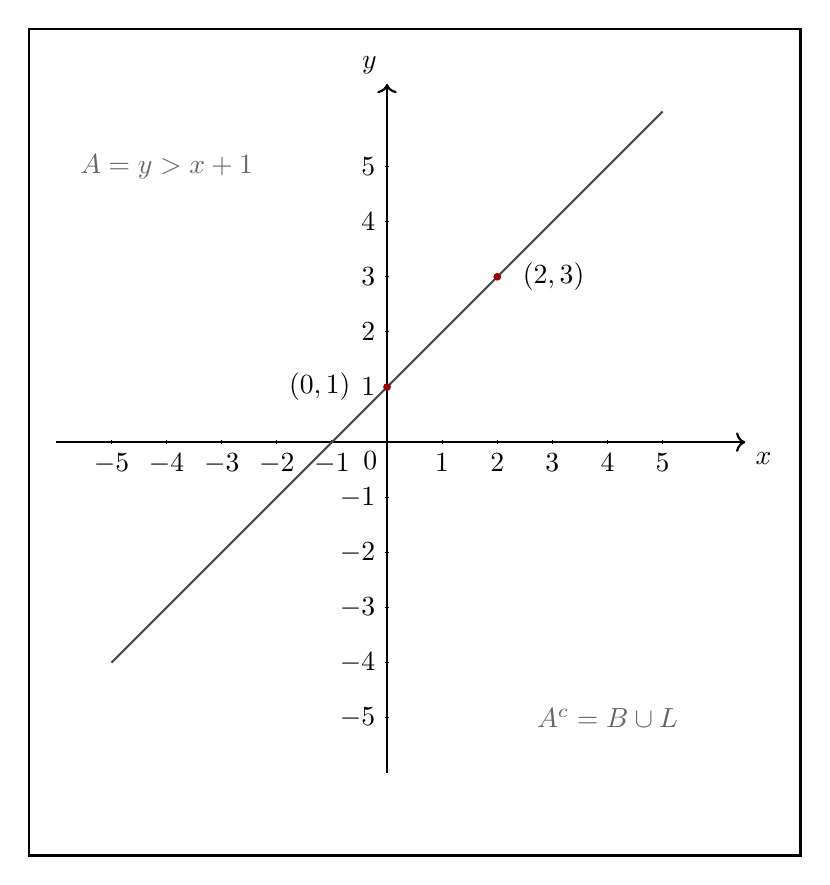
\begin{tikzpicture}[scale=0.7]
    % 
    \draw[thick,fill=white] (-6.5,-7.5) rectangle (7.5,7.5);

    % 
    \draw[thick,->] (-6,0) -- (6.5,0) node[anchor=north west] {$x$};
    \draw[thick,->] (0,-6) -- (0,6.5) node[anchor=south east] {$y$};
    \node[anchor=north east] at (0,0) {$0$};
    \foreach \x in {-5,-4,-3,-2,-1,1,2,3,4,5}
        \draw (\x cm,1pt) -- (\x cm,-1pt) node[anchor=north] {$\x$};
    \foreach \y in {-5, -4, -3,-2,-1,1,2,3,4,5}
        \draw (1pt,\y cm) -- (-1pt,\y cm) node[anchor=east] {$\y$};

    % 
    \draw[thick, gray!60!black] (-5,-4) -- (5,6);

    % 
    \fill[red!60!black] (2,3) circle (2pt);
    \node[right=2mm] at (2,3) {$(2,3)$};

    \fill[red!60!black] (0,1) circle (2pt);
    \node[left=2mm] at (-0.2,1) {$(0,1)$};

    % 
    \node[gray!80!black] at (-4,5) {$A = y > x + 1$};
    \node[gray!80!black] at (4,-5) {$A^c = B \cup L$};
\end{tikzpicture}
\end{center}

That is,
\[
\boxed{A^c = \displaystyle\bigcup_{x \in \mathbb{R}} \{\, (x, y) \in \mathbb{R}^2 \mid y \le x + 1 \,\}
\;=\; B \cup L }
\]

where
\[
B = \{\, (x, y) \in \mathbb{R}^2 \mid y < x + 1 \,\}, 
\quad
L = \{\, (x, y) \in \mathbb{R}^2 \mid y = x + 1 \,\}.
\]


\subsection{Cartesian Product}\label{CartesianProduct}

Symbolic notation for Cartesian Product is: $$
A \times B = \{ \langle a,b \rangle  \mid a \in A \wedge b \in B \}
$$

\textbf{Example 1:}

$$
\begin{aligned}
A &= \{0, 1\} \\
B &= \{1, a, b\}
\end{aligned}
$$

\begin{center}
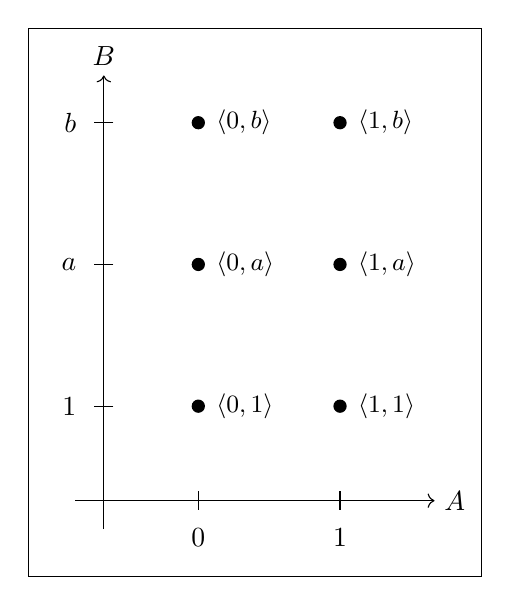
\begin{tikzpicture}[scale=1.2]
    % 
    \draw (-0.8,-0.8) rectangle (4,5);
    
    % 
    \draw[->] (-0.3,0) -- (3.5,0) node[right] {$A$};
    \draw[->] (0,-0.3) -- (0,4.5) node[above] {$B$};

    % 
    \foreach \x/\label in {1/0, 2.5/1} {
        \draw (\x,0.1) -- (\x,-0.1) node[below=3pt] {$\label$};
    }

    % 
    \foreach \y/\label in {1/1, 2.5/a, 4/b} {
        \draw (0.1,\y) -- (-0.1,\y) node[left=3pt] {$\label$};
    }

    % 
    \foreach \x in {1,2.5} {
        \foreach \y in {1,2.5,4} {
            \fill[black] (\x,\y) circle (2pt);
        }
    }

    % 
    \node[anchor=west, xshift=3pt] at (1,1) {\small$\langle 0,1 \rangle$};
    \node[anchor=west, xshift=3pt] at (1,2.5) {\small$\langle 0,a \rangle$};
    \node[anchor=west, xshift=3pt] at (1,4) {\small$\langle 0,b \rangle$};

    \node[anchor=west, xshift=3pt] at (2.5,1) {\small$\langle 1,1 \rangle$};
    \node[anchor=west, xshift=3pt] at (2.5,2.5) {\small$\langle 1,a \rangle$};
    \node[anchor=west, xshift=3pt] at (2.5,4) {\small$\langle 1,b \rangle$};
\end{tikzpicture}
\end{center}

Then the Cartesian product is  

$$
\begin{array}{|c|c|c|}
\hline
\langle 0,1 \rangle & \langle 0,a \rangle & \langle 0,b \rangle \\ \hline
\langle 1,1 \rangle & \langle 1,a \rangle & \langle 1,b \rangle \\ \hline
\end{array}
$$

\textbf{Example 2:}

Let  
$$
A = \{1, 2\}, \quad B = \{3, 4\}.
$$  

Hence
$$
\begin{array}{|c|c|}
\hline
\langle 1,3 \rangle & \langle 1,4 \rangle \\ \hline
\langle 2,3 \rangle & \langle 2,4 \rangle \\ \hline
\end{array}
$$


\textbf{Example 3:} 

Consider three sets:

$$
X = \{1, 2\}, \quad 
Y = \{a, b\}, \quad
Z = \{0, 9\}.
$$  

First, the Cartesian product of $X$ and $Y$:

$$
X \times Y = \{\langle 1,a \rangle, \langle 1,b \rangle, \langle 2,a \rangle, \langle 2,b \rangle\}
$$


Second, the Cartesian product of $(X \times Y)$ with $Z$ gives \textit{triplets}:

$$
\begin{array}{|c|c|}
\hline
\langle \langle 1,a \rangle, 0 \rangle & \langle \langle 1,a \rangle, 9 \rangle \\ \hline
\langle \langle 1,b \rangle, 0 \rangle & \langle \langle 1,b \rangle, 9 \rangle \\ \hline
\langle \langle 2,a \rangle, 0 \rangle & \langle \langle 2,a \rangle, 9 \rangle \\ \hline
\langle \langle 2,b \rangle, 0 \rangle & \langle \langle 2,b \rangle, 9 \rangle \\ \hline
\end{array}
$$


\textbf{Example 4:}

Let  
$$
A = \{1, 2\}, \quad B = \{3, 4\}, \quad C = \{5, 6\}, \quad D = \{7, 8\}.
$$  

The Cartesian product of these four sets, denoted  

$$
A \times B \times C \times D,
$$  

is the set of all ordered \textit{quadruples} where the first element comes from $A$, the second from $B$, the third from $C$, and the fourth from $D$.  

Explicitly:

$$
\begin{array}{|c|c|c|c|}
\hline
\langle \langle \langle 1,3 \rangle, 5 \rangle, 7 \rangle & \langle \langle \langle 1,3 \rangle, 5 \rangle, 8 \rangle & \langle \langle \langle 1,3 \rangle, 6 \rangle, 7 \rangle & \langle \langle \langle 1,3 \rangle, 6 \rangle, 8 \rangle \\ \hline
\langle \langle \langle 1,4 \rangle, 5 \rangle, 7 \rangle & \langle \langle \langle 1,4 \rangle, 5 \rangle, 8 \rangle & \langle \langle \langle 1,4 \rangle, 6 \rangle, 7 \rangle & \langle \langle \langle 1,4 \rangle, 6 \rangle, 8 \rangle \\ \hline
\langle \langle \langle 2,3 \rangle, 5 \rangle, 7 \rangle & \langle \langle \langle 2,3 \rangle, 5 \rangle, 8 \rangle & \langle \langle \langle 2,3 \rangle, 6 \rangle, 7 \rangle & \langle \langle \langle 2,3 \rangle, 6 \rangle, 8 \rangle \\ \hline
\langle \langle \langle 2,4 \rangle, 5 \rangle, 7 \rangle & \langle \langle \langle 2,4 \rangle, 5 \rangle, 8 \rangle & \langle \langle \langle 2,4 \rangle, 6 \rangle, 7 \rangle & \langle \langle \langle 2,4 \rangle, 6 \rangle, 8 \rangle \\ \hline
\end{array}
$$


\textbf{Example 5:}

$$
\begin{aligned}
A &= \left\{ (x, y) \in \mathbb{R}^2 \;\Bigm|\; \frac{1}{2} = \frac{y-1}{3x-4}\right\} \\
B &= \left\{ (x, y) \in \mathbb{Z}^2 \;\Bigm|\; x \ge 6y, \; x \neq 0 \right\}
\end{aligned}
$$

Therefore, 

$$
\begin{aligned}
A &=  \{ \langle 0, -1 \rangle, \langle 2/3, 0 \rangle, \langle 1, 0.5 \rangle, \dots \}\\
B &=  \{ \langle 1, 0 \rangle, \langle 6, 1 \rangle, \langle 12, 2 \rangle, \dots \}
\end{aligned}
$$

Then the Cartesian product $A \times B$ is all possible pairs combining one point from $A$ with one point from $B$:

$$
\begin{array}{|c|c|c|}
\hline
\langle \langle 0,-1 \rangle, \langle 1,0 \rangle \rangle & \langle \langle 0,-1 \rangle, \langle 6,1 \rangle \rangle & \langle \langle 0,-1 \rangle, \langle 12,2 \rangle \rangle \\ \hline
\langle \langle 2/3,0 \rangle, \langle 1,0 \rangle \rangle & \langle \langle 2/3,0 \rangle, \langle 6,1 \rangle \rangle & \langle \langle 2/3,0 \rangle, \langle 12,2 \rangle \rangle \\ \hline
\langle \langle 1,0.5 \rangle, \langle 1,0 \rangle \rangle & \langle \langle 1,0.5 \rangle, \langle 6,1 \rangle \rangle & \langle \langle 1,0.5 \rangle, \langle 12,2 \rangle \rangle \\ \hline
\end{array}
$$


Thus, the Cartesian product is:

$$
\boxed{
A \times B = \{ \bigl((x, \tfrac{3}{2}x - 1), (m,n)\bigr) \;\bigm|\; x \in \mathbb{R},\; m,n \in \mathbb{Z},\; m \ge 6n,\; m \neq 0 \}
}
$$

\subsection{Subset}\label{Subset}
The symbolic notation for subset is:

$$
A \subseteq B \leftrightarrow \forall x \, (x \in A \to x \in B)
$$

If $A$ is not a subset of $B$, we write $A \nsubseteq B$. This means that there exists at least one element in $A$ that is not in $B$:

$$
A \nsubseteq B \leftrightarrow \exists x \, (x \in A \land x \notin B)
$$

Furthermroe, It's crucial to distinguish between an element of a set and a subset of a set:

1. $2 \in \mathbb{Z}$

2. $\mathbb{E} \subseteq \mathbb{Z}$ (the set of even numbers is a subset of the integers)  

3. A set can be both an element and a subset of another set. 

For example:  

$$
\{1\} \in \{1, \{1\}\} \quad \text{and} \quad \{1\} \subseteq \{1, \{1\}\}
$$

This shows that a set can be both an element and a subset of another set:

\begin{enumerate}
  \item $\{1\} \in \{1, \{1\}\}$ means the set $\{1\}$ is listed as an element of the larger set.
  \item $\{1\} \subseteq \{1, \{1\}\}$ means every element of $\{1\}$ (which is just $1$) is also in the larger set.
\end{enumerate}

In contrast, the number $1$ itself is only an element, not a subset:

\begin{enumerate}
  \item $1 \in \{1, \{1\}\}$, because $1$ is directly in the set.
  \item $1 \nsubseteq \{1, \{1\}\}$ because $1$ is not a set and therefore cannot be a subset.
\end{enumerate}

\textbf{Example 1:}
Let  
\[
A = \{1,2,3,4,5\}, \quad B = \{2,4\}.
\]  

We check whether $B$ is a subset of $A$:

\[
B \subseteq A
\]  

Here, every element of $B$ is present in $A$, so $B$ is indeed a subset.

\textbf{Example 2:}

Consider three sets:

\[
X = \{10,20,30,40\}, \quad 
Y = \{10,20,30,40\}, \quad
Z = \{20,30\}.
\]  

$Y$ is a subset of $X$:

\[
Y \subseteq X
\]

$Z$ is also a subset of $X$:

\[
Z \subseteq X
\]


\textbf{Example 3:}

\[
A \subseteq B \;\to\; A \cup B = B
\]

\textit{Proof.}

By definition of subset:

\[
A \subseteq B \;\leftrightarrow\; \forall x \, (x \in A \to x \in B)
\]

By definition of union:

\[
A \cup B = \{x \mid x \in A \lor x \in B\}
\]

Thus:

\[
x \in A \cup B 
\;\leftrightarrow\;
(x \in A \lor x \in B)
\]

Since $A \subseteq B$, we know $\forall x \, (x \in A \to x \in B)$.  

Hence:

\[
x \in A \cup B
\;\leftrightarrow\;
(x \in A \lor x \in B)
\;\leftrightarrow\;
(x \in B \lor x \in B)
\;\leftrightarrow\;
x \in B
\]

Therefore:

\[
\boxed{A \cup B = B. \quad \text{QED}}
\]

\textbf{Example 4:}

\[
A \subseteq B \;\to\; A \cap B = A
\]

\textit{Proof.}

By definition of subset:

\[
A \subseteq B \;\leftrightarrow\; \forall x \, (x \in A \to x \in B)
\]

By definition of intersection:

\[
A \cap B = \{x \mid x \in A \land x \in B\}
\]

Thus:

\[
x \in A \cap B 
\;\leftrightarrow\;
(x \in A \land x \in B)
\]

But since $A \subseteq B$, if $x \in A$, then automatically $x \in B$.  

So:

\[
(x \in A \land x \in B) \;\leftrightarrow\; x \in A
\]

Therefore:

\[
\boxed{A \cap B = A. \quad \text{QED}}
\]

\textbf{Example 5:}

Let 

\[
A \subseteq \displaystyle\bigcup B
\]

\textit{Proof.}

By definition of subset:  

\[
A \subseteq \displaystyle\bigcup B \;\leftrightarrow\; \forall x \,(x \in A \to x \in \bigcup B)
\]  

By the definition of the union over a set of sets:

If $A$ is a set of sets, then  

\[
\displaystyle\bigcup A = \{\, x \mid x \text{ belongs to an element of } A \,\} 
= \{\, x \mid \exists C \in A \; (x \in C) \,\}.
\]  

Moreover, let $x \in A$.  

Since $A \in B$, we may take $C = A$ as one of the sets in $B$. Thus $x \in C$ with $C \in B$, which means $x \in \displaystyle\bigcup B$.  

Therefore:  

\[
\forall x \,(x \in A \to x \in \displaystyle\bigcup B),
\]  

so by the definition of subset:  

\[
\boxed{A \subseteq \displaystyle\bigcup B. \quad \text{QED}}
\]


\subsection{Power Set}\label{Power Set}

The symbolic notation for the power set of a set $A$ is:

$$
\mathcal{P}(A) = \{x \mid x \subseteq A\}
$$

\textbf{Example 1:}

Let  
\[
S = \{a, b\}.
\]  

Then the power set of $S$ is  
\[
\mathcal{P}(S) = \{\;\varnothing,\; \{a\},\; \{b\},\; \{a,b\}\;\}.
\]  

Since $|S| = 2$, the size of the power set is  
\[
\boxed{|\mathcal{P}(S)| = 2^{|S|} = 2^2}
\]


\textbf{Example 2:}

Let  
\[
Y = \varnothing.
\]  

That is, $Y$ is the empty set. Then the power set is  

\[
\mathcal{P}(Y) = \{\;\varnothing\;\}.
\]  

Here,  
\[
|\mathcal{P}(Y)| = 2^{|Y|} = 2^0 = 1.
\]  

So the power set of the empty set contains exactly one element, the empty set itself.


\textbf{Example 3:}

Let 
\[
\begin{aligned}
A &= \{1, 2, 3\}
\end{aligned}
\]
and we ask for 
\[
B = \{\mathcal{P}(\mathcal{P}(A))\}.
\]

For $\mathcal{P}(A)$,
\[
\mathcal{P}(A) = \{\varnothing, \{1\}, \{2\}, \{3\}, \{1,2\}, \{1,3\}, \{2,3\}, \{1,2,3\}\}.
\]

We have  
\[
|\mathcal{P}(A)| = 2^{|A|} = 2^3.
\]

Then for $B$,
\[
\boxed{|\mathcal{P}(\mathcal{P}(A))| = 2^{|\mathcal{P}(A)|} = 256.}
\]


\textbf{Example 4:}

Let  
\[
A = \{1,2\}, \quad \text{and} \quad B = \{3,4\}.
\]  

We ask for  
\[
C = \mathcal{P}(A) \times \mathcal{P}(B).
\]  

Since  
\[
|\mathcal{P}(A)| = 2^{|A|} 
\quad \text{and} \quad 
|\mathcal{P}(B)| = 2^{|B|},
\]  
it follows that  
\[
\boxed{|C| = 2^{|A|+|B|} = 16.}
\]

Explicitly,  
\[
\begin{array}{|c|c|c|c|}
\hline
(\varnothing,\varnothing) & (\varnothing,\{3\}) & (\varnothing,\{4\}) & (\varnothing,\{3,4\}) \\ \hline
(\{1\},\varnothing) & (\{1\},\{3\}) & (\{1\},\{4\}) & (\{1\},\{3,4\}) \\ \hline
(\{2\},\varnothing) & (\{2\},\{3\}) & (\{2\},\{4\}) & (\{2\},\{3,4\}) \\ \hline
(\{1,2\},\varnothing) & (\{1,2\},\{3\}) & (\{1,2\},\{4\}) & (\{1,2\},\{3,4\}) \\ \hline
\end{array}
\]


\textbf{Example 5:}

Let  
\[
A = \{\,x \in \mathcal{P}(\{1,2,3,4\}) \mid 2 \in x \,\}.
\]  

From that definition we know that  
\[
x \subseteq \{1,2,3,4\}, \quad \text{and } 2 \in x.
\]  

First, the power set of $\{1,2,3,4\}$ is:

\[
\begin{array}{|c|c|c|c|}
\hline
\varnothing & \{1\} & \{2\} & \{3\} \\ \hline
\{4\} & \{1,2\} & \{1,3\} & \{1,4\} \\ \hline
\{2,3\} & \{2,4\} & \{3,4\} & \{1,2,3\} \\ \hline
\{1,2,4\} & \{1,3,4\} & \{2,3,4\} & \{1,2,3,4\} \\ \hline
\end{array}
\]

Now, we only select those subsets that contain 2.  

Thus,  
\[
\begin{array}{|c|c|c|c|}
\hline
\{2\} & \{1,2\} & \{2,3\} & \{2,4\} \\ \hline
\{1,2,3\} & \{1,2,4\} & \{2,3,4\} & \{1,2,3,4\} \\ \hline
\end{array}
\]

Hence the set has  
\[
\boxed{|A| = 8.}
\]

% ===== PART 22 =====%
\section{Relations Order}

\subsection{Preorder}

A relation $R \subseteq A^2$ is a preorder if

$$
\forall x \in A, \ xRx \quad
$$

$$
\forall x,y,z \in A, \ (xRy \land yRz) \implies xRz
$$

Let $A = \{a,b,c\}$. The Cartesian product is

$$
\begin{array}{c|ccc}
A^2 & a & b & c \\
\hline
a & (a,a) & (a,b) & (a,c) \\
b & (b,a) & (b,b) & (b,c) \\
c & (c,a) & (c,b) & (c,c) \\
\end{array}
$$

\textbf{Example 1:}

$$
R = \{(a,a),(b,b),(c,c),(a,b),(b,a)\}
$$

Reflexive:

$$
\forall x \in A, (x,x) \in R
$$

Transitive:

$$
\forall x,y,z \in A, (xRy \land yRz) \implies xRz
$$

But not antisymmetric:

$$
aRb \land bRa \quad \text{but} \quad a \neq b
$$

\textbf{Example 2:}

Universal relation on $L = \{a,b\}$

$$
R = L^2
$$

Reflexive, transitive, but not antisymmetric if $|L|>1$.

\subsection{Partial Order}

A relation $R \subseteq A^2$ is a partial order if

$$\forall x \in A, \ xRx$$

$$\forall x,y,z \in A, \ (xRy \land yRz) \implies xRz$$

$$\forall x,y \in A, \ (xRy \land yRx) \implies x=y$$

\textbf{Example 1:}

Let $A = \{a,b,c\}$

$$
\begin{array}{c|ccc}
A^2 & a & b & c \\
\hline
a & (a,a) & (a,b) & (a,c) \\
b & (b,a) & (b,b) & (b,c) \\
c & (c,a) & (c,b) & (c,c) \\
\end{array}
$$

$$
R = \{(a,a),(b,b),(c,c),(a,b),(a,c)\}
$$

Reflexive, transitive, antisymmetric, but not connected:

$$
\neg(bRc) \land \neg(cRb)
$$

\textbf{Example 2:}

$$
A = \mathcal{P}(\{a,b\}) = \{\varnothing,\{a\},\{b\},\{a,b\}\}
$$

$$
\begin{array}{c|cccc}
A^2 & \varnothing & \{a\} & \{b\} & \{a,b\} \\
\hline
\varnothing & (\varnothing,\varnothing) & (\varnothing,\{a\}) & (\varnothing,\{b\}) & (\varnothing,\{a,b\}) \\
\{a\} & (\{a\},\varnothing) & (\{a\},\{a\}) & (\{a\},\{b\}) & (\{a\},\{a,b\}) \\
\{b\} & (\{b\},\varnothing) & (\{b\},\{a\}) & (\{b\},\{b\}) & (\{b\},\{a,b\}) \\
\{a,b\} & (\{a,b\},\varnothing) & (\{a,b\},\{a\}) & (\{a,b\},\{b\}) & (\{a,b\},\{a,b\}) \\
\end{array}
$$

$$
R = \subseteq
$$

Reflexive, transitive, antisymmetric, but not connected:

$$
\{a\} \nsubseteq \{b\}, \quad \{b\} \nsubseteq \{a\}
$$

\textbf{Example 3:}

Divisibility on $\mathbb{N}$

$$
n \mid m \leftrightarrow \exists k \in \mathbb{N}, m = kn
$$

Partial order, not linear:

$$
2 \nmid 3, \quad 3 \nmid 2
$$

On $\mathbb{Z}$, not antisymmetric:

$$
1 \mid -1 \land -1 \mid 1 \quad \text{but} \quad 1 \neq -1
$$

\subsection{Linear Order}

A relation $R \subseteq A^2$ is a linear order if it is a partial order and

$$
\forall x,y \in A, \ x \neq y \implies (xRy \lor yRx)
$$

\textbf{Example 1:}

Let $A = \{a,b,c\}$

$$
\begin{array}{c|ccc}
A^2 & a & b & c \\
\hline
a & (a,a) & (a,b) & (a,c) \\
b & (b,a) & (b,b) & (b,c) \\
c & (c,a) & (c,b) & (c,c) \\
\end{array}
$$

$$
R = \{(a,a),(b,b),(c,c),(a,b),(b,c),(a,c)\}
$$

Reflexive, transitive, antisymmetric, connected: corresponds to $a < b < c$.

\textbf{Example 2:}

$$ x \leq y \leftrightarrow x = y \vee x < y $$

Reflexive, transitive, antisymmetric, connected: $(\mathbb{N}, \leq)$ is a linear order.

\subsection{Strict Order}

A relation $R \subseteq A^2$ is a strict order if

$$ \forall x \in A, \ \neg(xRx)$$

$$\forall x,y \in A, \ xRy \implies \neg(yRx)$$

$$\forall x,y,z \in A, \ (xRy \land yRz) \implies xRz$$

\textbf{Example 1:}

Let $A = \{a,b,c\}$

$$
\begin{array}{c|ccc}
A^2 & a & b & c \\
\hline
a & (a,a) & (a,b) & (a,c) \\
b & (b,a) & (b,b) & (b,c) \\
c & (c,a) & (c,b) & (c,c) \\
\end{array}
$$

$$
R = \{(a,b),(a,c),(b,c)\}
$$

Irreflexive, asymmetric, transitive.

\textbf{Example 2:}

$$
x < y \leftrightarrow \exists k \in \mathbb{N}^+, \ y = x+k
$$

Irreflexive, asymmetric, transitive: $(\mathbb{N},<)$ is a strict order.

\subsection{Strict Linear Order}

A strict linear order is a strict order that is connected:

$$
\forall x,y \in A, \ x \neq y \implies (xRy \lor yRx)
$$

\textbf{Example 1:}

Let $A = \{a,b,c\}$

$$
\begin{array}{c|ccc}
A^2 & a & b & c \\
\hline
a & (a,a) & (a,b) & (a,c) \\
b & (b,a) & (b,b) & (b,c) \\
c & (c,a) & (c,b) & (c,c) \\
\end{array}
$$

$$
R = \{(a,b),(a,c),(b,c)\}
$$

Irreflexive, asymmetric, transitive, connected: corresponds to $a < b < c$.

\textbf{Example 2:}

$$
x < y \leftrightarrow \exists k \in \mathbb{N}^+, \ y = x+k
$$

Irreflexive, asymmetric, transitive, connected: $(\mathbb{N},<)$ is a strict linear order.

\begin{enumerate}
\item $3 \not< 3$
\item $2 < 5$, then $5 \not< 2$
\item $1 < 4 \land 4 < 7 \implies 1 < 7$
\item $6 \neq 10 \implies (6 < 10 \lor 10 < 6)$
\end{enumerate}

\textbf{Example 3:}

$$
X \subsetneq Y \leftrightarrow X \subseteq Y \land X \neq Y
$$

\begin{enumerate}
\item $\{1\} \subsetneq \{1, 2\}$
\item $\{1, 2\} \subsetneq \{1, 2, 3\}$
\item $\{1, 2\} \not\subsetneq \{1, 2\}$
\end{enumerate}

If $<$ is a strict linear order on $A$, then

$$
\forall a,b \in A, \ \big[ (\forall x \in A, \ x < a \leftrightarrow x < b) \implies a = b \big]
$$

\textbf{Example :}

For $A = \{a,b,c\}$ with $< = \{(a,b),(a,c),(b,c)\}$:

$$
\{ x \in A \mid x < a \} = \varnothing, \quad
\{ x \in A \mid x < b \} = \{a\}, \quad
\{ x \in A \mid x < c \} = \{a,b\}
$$

\textit{Property:}

\begin{enumerate}
\item If $R$ is a strict order on $A$, then

    $$
    R^+ = R \cup \text{Id}_A
    $$

    is a partial order. Moreover, if $R$ is a strict linear order, then $R^+$ is a linear order.

\item If $R$ is a partial order on $A$, define

    $$
    R^- = R \setminus \text{Id}_A
    $$

    $R^-$ is a strict order (irreflexive, asymmetric, transitive). Moreover, if $R$ is a linear order, then $R^-$ is a strict linear order.
\end{enumerate}

\textbf{Example:}

Let $A = \{a,b,c\}$ and

$$
R = \{(a,b),(a,c),(b,c)\} \quad \text{(strict linear order)}
$$

The Cartesian product $A^2$:

$$
\begin{array}{c|ccc}
A^2 & a & b & c \\
\hline
a & (a,a) & (a,b) & (a,c) \\
b & (b,a) & (b,b) & (b,c) \\
c & (c,a) & (c,b) & (c,c) \\
\end{array}
$$

Identity relation:

$$
\text{Id}_A = \{(a,a),(b,b),(c,c)\}
$$

Then  

$$
R^+ = R \cup \text{Id}_A = \{(a,a),(b,b),(c,c),(a,b),(a,c),(b,c)\}
$$

$$
R^- = R^+ \setminus \text{Id}_A = \{(a,b),(a,c),(b,c)\}
$$

$R^+$ is a linear order, and $R^-$ is a strict linear order.



% ===== PART 23 =====%
\section{Operations on Relations}

Let $R, S \subseteq A^2$ be binary relations on a set $A$. The following are standard operations on relations:

\subsection{Inverse of a Relation}

Definition:

$$
R^{-1} = \{ \langle y, x \rangle \mid \langle x, y \rangle \in R \}
$$

In general, if $R \subseteq \mathbb{N}^2$, the inverse relation $R^{-1}$ contains all pairs of $R$ with their coordinates swapped:

$$
R^{-1} = \{ (y, x) \in \mathbb{N}^2 \mid (x, y) \in R \}
$$

Example:

Let $$S = \{ \langle x, y \rangle \in \mathbb{Z}^2 \mid x + 1 = y \}$$

That is,

$$
\begin{array}{c|ccccccc}
S & \cdots & -1 & 0 & 1 & 2 & 3 & \cdots \\
\hline
\vdots & \ddots & \vdots & \vdots & \vdots & \vdots & \vdots & \\
-1 & \cdots & & (-1,0) & & & & \cdots \\
0 & \cdots & & & (0,1) & & & \cdots \\
1 & \cdots & & & & (1,2) & & \cdots \\
2 & \cdots & & & & & (2,3) & \cdots \\
\vdots & & \vdots & \vdots & \vdots & \vdots & \vdots & \ddots \\
\end{array}
$$

Then:

$$
\begin{array}{c|ccccccc}
S^{-1} & \cdots & -2 & -1 & 0 & 1 & 2 & \cdots \\
\hline
\vdots & \ddots & \vdots & \vdots & \vdots & \vdots & \vdots & \\
0 & \cdots & & (0,-1) & & & & \cdots \\
1 & \cdots & & & (1,0) & & & \cdots \\
2 & \cdots & & & & (2,1) & & \cdots \\
3 & \cdots & & & & & (3,2) & \cdots \\
\vdots & & \vdots & \vdots & \vdots & \vdots & \vdots & \ddots \\
\end{array}
$$

\subsection{Relative Product of Relations}

Definition:

$$
(R \mid S) = \{ \langle x, z \rangle \mid \exists y \, (xRy \wedge ySz) \}
$$

Example:

Suppose we have:  

$$
R = \{ (1, 2), (2, 3), (3, 4) \}, \quad
S = \{ (2, 5), (3, 6), (4, 7) \}
$$

Then the composition of relations is:

$$
R \mid S = \{ (x, z) \mid \exists y \, ((x, y) \in R \wedge (y, z) \in S) \}
$$

Thus:

\begin{enumerate}
\item $((1, 2) \in R) \text{ and } ((2, 5) \in S) \to ((1, 5) \in R \mid S)$ 
\item $((2, 3) \in R) \text{ and } ((3, 6) \in S) \to ((2, 6) \in R \mid S)$  
\item $((3, 4) \in R) \text{ and } ((4, 7) \in S) \to ((3, 7) \in R \mid S)$
\end{enumerate}

Consequently:

$$
R \mid S = \{ (1, 5), (2, 6), (3, 7) \}
$$

\subsection{Restriction of a Relation}

Definition:

$$
R \upharpoonright A = R \cap A^2
$$

In general, if $R \subseteq \mathbb{N}^2$ and $A \subseteq \mathbb{N}$, the restriction of $R$ to $A$ keeps only those pairs in $R$ where both elements are in $A$:

$$
R \upharpoonright A = \{ (x, y) \in R \mid (x,y) \in A \}
$$

Hence:

$$
\begin{array}{c|cccc}
A^2 & a_1 & a_2 & \dots & a_n \\
\hline
a_1 & (a_1,a_1) & (a_1,a_2) & \dots & (a_1,a_n) \\
a_2 & (a_2,a_1) & (a_2,a_2) & \dots & (a_2,a_n) \\
\vdots & \vdots & \vdots & \vdots & \vdots \\
a_n & (a_n,a_1) & (a_n,a_2) & \dots & (a_n,a_n) \\
\end{array}
$$

Example 1:

Given:

$$R = \{(1, 2), (2, 4), (3, 6), (4, 8), (5, 10), (6, 12)\} \subseteq \mathbb{Z}^2$$

Restriction to even numbers $E = \{2, 4, 6, 8, 10, 12, \ldots\}$:

$$R \upharpoonright_E = \{(2, 4), (4, 8), (6, 12)\}$$


Example 2:

Given:
$$f = \{(x, x^2) \mid x \in \mathbb{R}\}$$


Restriction to $\mathbb{Z} \cap [0,3]$:

$$
\begin{array}{c|cccc}
f \upharpoonright_{\mathbb{Z} \cap [0,3]} & 0 & 1 & 2 & 3 \\
\hline
0 & (0,0) & & & \\
1 & & (1,1) & & \\
2 & & & (2,4) & \\
3 & & & & (3,9) \\
\end{array}
$$

Example 3:

Let

$$
\begin{array}{c|ccccccc}
\mathbb{R}^2 & \cdots & a_{ijk} & \cdots & b_{lmn} & \cdots & c_{pqr} & \cdots \\
\hline
\vdots & \vdots & \vdots & \vdots & \vdots & \vdots & \vdots & \vdots \\
a_{ijk} & \cdots & (a_{ijk},a_{ijk}) & \cdots & (a_{ijk},b_{lmn}) & \cdots & (a_{ijk},c_{pqr}) & \cdots \\
\vdots & \vdots & \vdots & \vdots & \vdots & \vdots & \vdots & \vdots \\
b_{lmn} & \cdots & (b_{lmn},a_{ijk}) & \cdots & (b_{lmn},b_{lmn}) & \cdots & (b_{lmn},c_{pqr}) & \cdots \\
\vdots & \vdots & \vdots & \vdots & \vdots & \vdots & \vdots & \vdots \\
c_{pqr} & \cdots & (c_{pqr},a_{ijk}) & \cdots & (c_{pqr},b_{lmn}) & \cdots & (c_{pqr},c_{pqr}) & \cdots \\
\vdots & \vdots & \vdots & \vdots & \vdots & \vdots & \vdots & \vdots \\
\end{array}
$$

Restriction to $\mathbb{N}^2$:

$$
\begin{array}{c|cccc}
\mathbb{N}^2 & 1 & 2 & 3 & \cdots \\
\hline
1 & (1,1) & (1,2) & (1,3) & \cdots \\
2 & (2,1) & (2,2) & (2,3) & \cdots \\
3 & (3,1) & (3,2) & (3,3) & \cdots \\
\vdots & \vdots & \vdots & \vdots & \ddots \\
\end{array}
$$

Given relation:
$$R = \{(a_{ijk}, c_{pqr}), (b_{lmn}, 2), (2, 3), (\pi, e), (3, 5)\} \subseteq \mathbb{R}^2$$

Restriction to $\mathbb{N}^2$:
$$R \upharpoonright_{\mathbb{N}^2} = \{(2, 3), (3, 5)\}$$

\subsection{Application of a Relation to a Set}

Definition:

$$
R[A] = \{ y \in A \mid \exists x \in A, \langle x, y \rangle \in R \}
$$

Example:

Let $$S = \{ (a,b), (b,c), (c,d) \}$$

and consider the set $P = \{a,b,c\}$.

Where:

$$\begin{aligned}
   (a,b) &\to b \in S[\cdot]\\
    (b,c) &\to c \in S[\cdot]\\
    (c,d) &\to d \notin S[P] \text{ since } d \notin P
\end{aligned}
$$  

Then:

$$
S[P] = \{b,c\}
$$

\subsection{Transitive Closure}

Definition:

$$
R^1 = R, \quad R^{n+1} = R^n \mid R
$$

$$
R^+ = \displaystyle\bigcup_{n=1}^{\infty} R^n
$$

Example:

Let $$R = \{ (1,2), (2,3), (3,4) \}$$ 

Since:

$$\begin{aligned}
R^1 =& \{ (1,2), (2,3), (3,4) \} \\
R^2 =& R \mid R = \{ (1,3), (2,4) \} \\
R^3 =& R^2 \mid R = \{ (1,4) \}
\end{aligned}$$

Therefore:

$$
\begin{array}{c|cccc}
R^+ & 1 & 2 & 3 & 4 \\
\hline
1 & & (1,2) & (1,3) & (1,4) \\
2 & & & (2,3) & (2,4) \\
3 & & & & (3,4) \\
4 & & & & \\
\end{array}
$$

\subsection{Reflexive Transitive Closure}

Definition:

Let $$\text{Id}_A = \{ \langle x, x \rangle \mid x \in A \}$$

then

$$
R^* = R^+ \cup \text{Id}_A
$$

Example:

Since $\text{Id}_A$:

$$
\begin{array}{c|cccc}
\text{Id}_A & 1 & 2 & 3 & 4 \\
\hline
1 & (1,1) & & & \\
2 & & (2,2) & & \\
3 & & & (3,3) & \\
4 & & & & (4,4) \\
\end{array}
$$

We conclude that,
$
R^* = R^+ \cup \text{Id}_A
$:

$$
\begin{array}{c|cccc}
R^* & 1 & 2 & 3 & 4 \\
\hline
1 & (1,1) & (1,2) & (1,3) & (1,4) \\
2 & & (2,2) & (2,3) & (2,4) \\
3 & & & (3,3) & (3,4) \\
4 & & & & (4,4) \\
\end{array}
$$

% ===== PART 24 =====%
\section{Set Properties and Laws}

\subsection{Commutative Laws}

\begin{enumerate}
    \item $A \cup B = B \cup A$
    \item $A \cap B = B \cap A$
\end{enumerate}

Let $A = \{1, 2, 3\}$ and $B = \{3, 4, 5\}$.

\[
\begin{array}{|l|c|}
\hline
\text{Operation} & \text{Result} \\ \hline
A \cup B & \{1, 2, 3, 4, 5\} \\ \hline
B \cup A & \{1, 2, 3, 4, 5\} \\ \hline
A \cap B & \{3\} \\ \hline
B \cap A & \{3\} \\ \hline
\end{array}
\]


\subsection{Associative Laws}

\begin{enumerate}
    \item $(A \cup B) \cup C = A \cup (B \cup C)$
    \item $(A \cap B) \cap C = A \cap (B \cap C)$
\end{enumerate}

Let $A = \{1, 2\}$, $B = \{2, 3\}$, and $C = \{3, 4\}$.

\[
\begin{array}{|l|c|}
\hline
\text{Operation} & \text{Result} \\ \hline
(A \cup B) \cup C & \{1, 2, 3, 4\} \\ \hline
A \cup (B \cup C) & \{1, 2, 3, 4\} \\ \hline
(A \cap B) \cap C & \varnothing \\ \hline
A \cap (B \cap C) & \varnothing \\ \hline
\end{array}
\]


\subsection{Distributive Laws}

\begin{enumerate}
    \item $A \cup (B \cap C) = (A \cup B) \cap (A \cup C)$
    \item $A \cap (B \cup C) = (A \cap B) \cup (A \cap C)$
\end{enumerate}

Let $A = \{1, 2\}$, $B = \{2, 3\}$, and $C = \{3, 4\}$.

\[
\begin{array}{|l|c|}
\hline
\text{Operation} & \text{Result} \\ \hline
A \cup (B \cap C) & \{1, 2, 3\} \\ \hline
(A \cup B) \cap (A \cup C) & \{1, 2, 3\} \\ \hline
A \cap (B \cup C) & \{2\} \\ \hline
(A \cap B) \cup (A \cap C) & \{2\} \\ \hline
\end{array}
\]


\subsection{De Morgan's Laws}

\begin{enumerate}
    \item $(A \cup B)^c = A^c \cap B^c$
    \item $(A \cap B)^c = A^c \cup B^c$
\end{enumerate}

Let $U = \{1, 2, 3, 4, 5\}$, $A = \{1, 2\}$, and $B = \{2, 3\}$.

First, find the complements:  
$A^c = \{3, 4, 5\}$ and $B^c = \{1, 4, 5\}$.

\[
\begin{array}{|l|c|}
\hline
\text{Operation} & \text{Result} \\ \hline
(A \cup B)^c & \{4, 5\} \\ \hline
A^c \cap B^c & \{4, 5\} \\ \hline
(A \cap B)^c & \{1, 3, 4, 5\} \\ \hline
A^c \cup B^c & \{1, 3, 4, 5\} \\ \hline
\end{array}
\]


\subsection{Identity Laws}

\begin{enumerate}
    \item $A \cup \varnothing = A$
    \item $A \cap U = A$
\end{enumerate}

Let $U = \{1, 2, 3, 4, 5\}$ and $A = \{2, 3, 4\}$.

\[
\begin{array}{|l|c|}
\hline
\text{Operation} & \text{Result} \\ \hline
A \cup \varnothing & \{2, 3, 4\} \\ \hline
A \cap U & \{2, 3, 4\} \\ \hline
\end{array}
\]


\subsection{Idempotent Laws}

\begin{enumerate}
    \item $A \cup A = A$
    \item $A \cap A = A$
\end{enumerate}

Let $A = \{1, 3, 5\}$.

\[
\begin{array}{|l|c|}
\hline
\text{Operation} & \text{Result} \\ \hline
A \cup A & \{1, 3, 5\} \\ \hline
A \cap A & \{1, 3, 5\} \\ \hline
\end{array}
\]


\subsection{Complement Laws}

\begin{enumerate}
    \item $A \cup A^c = U$
    \item $A \cap A^c = \varnothing$
    \item $(A^c)^c = A$
\end{enumerate}

Let $U = \{1, 2, 3, 4, 5\}$ and $A = \{1, 3, 5\}$.  
First, find the complement: $A^c = \{2, 4\}$.

\[
\begin{array}{|l|c|}
\hline
\text{Operation} & \text{Result} \\ \hline
A \cup A^c & \{1, 2, 3, 4, 5\} = U \\ \hline
A \cap A^c & \varnothing \\ \hline
(A^c)^c & \{1, 3, 5\} = A \\ \hline
\end{array}
\]


\subsection{Absorption Laws}

\begin{enumerate}
    \item $A \cup (A \cap B) = A$
    \item $A \cap (A \cup B) = A$
\end{enumerate}

Let $A = \{1, 2, 3\}$ and $B = \{2, 3, 4\}$.

\[
\begin{array}{|l|c|}
\hline
\text{Operation} & \text{Result} \\ \hline
A \cup (A \cap B) & \{1, 2, 3\} \\ \hline
A \cap (A \cup B) & \{1, 2, 3\} \\ \hline
\end{array}
\]


% ===== PART 25 =====%

\section{Function}

A \textit{function} $f$ from set $A$ to set $B$ is a relation that assigns to each element of $A$ exactly one element of $B$.

Let $A$ and $B$ be sets. A function $f: A \to B$ is a subset $f \subseteq A \times B$ such that:

\[
f = \{(x, y) \in A \times B \mid f(x) = y \}
\]

This is a subset of $A \times B$ such that for every $x \in A$, there exists a unique $y \in B$ with $(x, y) \in f$.

\textbf{Example:}

Let $f: \mathbb{R} \to \mathbb{R}$ be defined by $x = 3.$

\[
f(x) = x + 2
\]

Then:

\[
f(3) = 3 + 2 = 5
\]

We conclude that:

\[
f(3) = 5
\]

This means the ordered pair $(3, 5) \in f$.

\subsection{Components}

\textbf{Domain:}
\[
\text{dom}(f) = A = \{x \mid \exists y \in B : (x, y) \in f\}
\]

\textbf{Codomain:}

\[
\text{cod}(f) = B
\]

\textbf{Range (Image):}

\[
\text{range}(f) = \text{im}(f) = \{y \in B \mid \exists x \in A : f(x) = y\}
\]

\textbf{Image of a subset:}

For $S \subseteq A$:

\[
f(S) = \{f(x) \mid x \in S\} = \{y \in B \mid \exists x \in S : f(x) = y\}
\]

\textbf{Preimage (Inverse Image):}

For $T \subseteq B$:

\[
f^{-1}(T) = \{x \in A \mid f(x) \in T\}
\]

\textbf{Example:}

Let

\[\begin{aligned}
A &= \{1, 2, 3, 4, 5\}\\
B &= \{0, 1, 2, 3, 4, 5, 6, 7, 8, 9, 10\}
\end{aligned}\]

Define

\[f: A \to B, \ f(x) = 2x\]

Let \[S = \{1, 3, 5\} \subseteq A\]

Then \[f(S) = \{f(x) \mid x \in S\}\]

\[\begin{aligned}
f(1) &= 2\\
f(3) &= 6\\
f(5) &= 10
\end{aligned}\]

Therefore 
\[
\boxed{f(S) = \{2, 6, 10\}}
\]

\textbf{Example 1:}

Let $f : \mathbb{R} \to \mathbb{R}$ be defined by $f(x) = x^2$.

\[
\text{range}(f) = \{y \in \mathbb{R} \mid y \geq 0\} = [0, \infty)
\]

Image of a set:

\[
f(\{-2, 3\}) = \{(-2)^2, 3^2\} = \{4, 9\}
\]

Preimage of a set:

\[
f^{-1}(\{4\}) = \{x \in \mathbb{R} \mid x^2 = 4\} = \{-2, 2\}
\]

\textbf{Example 2:}

Let

\[
\times : \mathbb{N} \times \mathbb{N} \to \mathbb{N}
\]

be the usual multiplication function defined by

\[
\times(a, b) = a \times b
\]

Then:

\[
\text{dom}(\times) = \mathbb{N} \times \mathbb{N}, \quad
\text{cod}(\times) = \mathbb{N}, \quad
\text{range}(\times) = \mathbb{N}
\]

For example:

\[
(3, 4) \in \mathbb{N} \times \mathbb{N}
\]

and

\[
3 \times 4 = 12
\]

Thus,

\[
\times(3, 4) = 12
\]

We also have the identity property:

\[
\forall n \in \mathbb{N}, \; \exists (n, 1) \in \mathbb{N} \times \mathbb{N} : n \times 1 = n
\]

\textbf{Example 3:}

Let
\[
f(x) = x^2 - 3x + 2
\]

We want to find

\[
f(2 + x)
\]

Substitute $2 + x$ for $x$:

\[
f(2 + x) = (2 + x)^2 - 3(2 + x) + 2
\]

Expand and simplify:

\begin{align*}
f(2 + x) &= (x^2 + 4x + 4) - 3(2 + x) + 2 \\
&= x^2 + 4x + 4 - 6 - 3x + 2 \\
&= x^2 + x
\end{align*}

So:
\[
\boxed{f(2 + x) = x^2 + x}
\]

\textbf{Example 4:}

Let
\[
f(x) = 2x + 3
\]

We want to find

\[
f^{-1}(x)
\]

We define

\begin{align*}
y &= 2x + 3 \\
y - 3 &= 2x \\
x &= \frac{y - 3}{2}
\end{align*}

Now, interchange $x$ and $y$:

\[
\boxed{f^{-1}(x) = \frac{x - 3}{2}}
\]

\textbf{Example 5:}

Let 
\[
f : \mathbb{N} \to \mathbb{N}
\]
be defined by
\[
f(x) = x + 1
\]

Then:

\[
\text{range}(f) = \mathbb{Z}^+ = \{1, 2, 3, \ldots\}
\]

For example:
\[
f(0) = 1, \quad f(1) = 2, \quad f(2) = 3
\]

Hence,
\[
0 \notin \text{range}(f) \text{ since } \nexists x \in \mathbb{N} : f(x) = 0
\]

\textbf{Example 6:}

Let $g : \mathbb{N} \to \mathbb{N}$ be defined by:

\[
g(x) = x + 2 - 1
\]

Then:

\[
\forall x \in \mathbb{N}, \; f(x) = x + 1 = x + 2 - 1 = g(x)
\]

By the principle of extensionality for functions:

\[
\forall x \in \text{dom}(f) : f(x) = g(x) \implies f = g
\]

provided $\text{dom}(f) = \text{dom}(g)$ and $\text{cod}(f) = \text{cod}(g)$.

\textbf{Example 7:}

Let $h : \mathbb{N} \to \mathbb{N}$ be defined by:

\[
h(x) = \begin{cases}
\frac{x}{2} & \text{if } x \text{ is even} \\[0.5em]
\frac{x + 1}{2} & \text{if } x \text{ is odd}
\end{cases}
\]

Since:

\[
\forall x \in \mathbb{N}, \; ( \text{even}(x) \lor \text{odd}(x)) \land \neg(\text{even}(x) \land\text{odd}(x))
\]

the function $h$ is well-defined and $h(x) \in \mathbb{N}$ for all $x \in \mathbb{N}$.

\subsection{Types of Functions}

\subsubsection{Injective}

A function $f : A \rightarrow B$ is injective or one-to-one if and only if:

\[
\forall x_1, x_2 \in A,\ f(x_1) = f(x_2) \Longrightarrow x_1 = x_2.
\]

Equivalently, for each $y \in B$, there is at most one $x \in A$ such that $f(x) = y$.

We call such a function an injection from $A$ to $B$.

\begin{center}
\fbox{
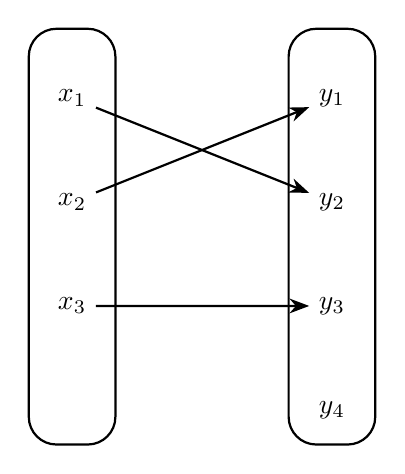
\begin{tikzpicture}[scale=1.1, every node/.style={scale=1}]


\draw[thick, rounded corners=10pt] (-0.5,-2.8) rectangle (0.5,2);


\draw[thick, rounded corners=10pt] (2.5,-2.8) rectangle (3.5,2);

\node (A1) at (0,1.2) {$x_1$};
\node (A2) at (0,0) {$x_2$};
\node (A3) at (0,-1.2) {$x_3$};

\node (B1) at (3,1.2) {$y_1$};
\node (B2) at (3,0) {$y_2$};
\node (B3) at (3,-1.2) {$y_3$};
\node (B4) at (3,-2.4) {$y_4$};

\draw[-{Stealth[length=2.5mm]}, thick] (A1) -- (B2);
\draw[-{Stealth[length=2.5mm]}, thick] (A2) -- (B1);
\draw[-{Stealth[length=2.5mm]}, thick] (A3) -- (B3);
\end{tikzpicture}
}
\end{center}
\newpage
\textbf{Example:}

\begin{enumerate}
\item $f : \mathbb{R} \to \mathbb{R}$, where $f(x) = 2x + 3$

   If $2x_1 + 3 = 2x_2 + 3$, then $x_1 = x_2$.

   Exponential function is strictly increasing.

\item $f : \mathbb{Z} \to \mathbb{N}$, defined by

   \[
   f(x) =
   \begin{cases}
   2x, & \text{if } x \ge 0, \\
   -2x - 1, & \text{if } x < 0
   \end{cases}
   \]

\item There exist injective functions from $\mathbb{N}$ into each of $\mathbb{N}, \mathbb{Z}, \mathbb{Q}, \mathbb{R}$.
   Formally:
   \[
   \exists f_i : \mathbb{N} \to S_i, \quad S_i \in \{\mathbb{N}, \mathbb{Z}, \mathbb{Q}, \mathbb{R}\}, \text{ such that } f_i \text{ is injective.}
   \]
   Example:

    \[
    \begin{aligned}
    f_1 &: \mathbb{N} \to \mathbb{N}, & f_1(x) &= x + 1 \\
    f_2 &: \mathbb{N} \to \mathbb{Z}, & 
    f_2(x) &=
    \begin{cases}
    \frac{x}{2}, & \text{if } x \text{ is even} \\[0.5em]
    -\frac{x+1}{2}, & \text{if } x \text{ is odd}
    \end{cases} \\
    f_3 &: \mathbb{N} \to \mathbb{Q}, & f_3(x) &= \frac{x}{x+1} \\
    f_4 &: \mathbb{N} \to \mathbb{R}, & f_4(x) &= x.
    \end{aligned}
    \]

    Each $f_i$ is injective, since distinct natural numbers map to distinct elements of the codomain.
\end{enumerate}


\textbf{Example:}

Let  \[f: \{2n+1 \mid n \in \mathbb{N}\} \longrightarrow \mathbb{Q}, \quad f(2n+1) = \frac{2n+1}{2n+2}\]

\[\operatorname{Im}(f) = \left\{\, \frac{a}{b} \in \mathbb{Q} \;\middle|\; a \in \{2n+1 \mid n \in \mathbb{N}\},\ b = a+1 \,\right\}\]

Hence,

\[
\begin{aligned}
f(1) &= 1/2 \\
f(3) &= 3/4 \\
f(5) &= 5/6 \\
f(7) &= 7/8 \\
f(9) &= 9/10 \\
&\vdots
\end{aligned}
\]

\subsubsection{Surjective}

A function $f : A \rightarrow B$ is surjective or onto if and only if $B$ is the range of $f$, i.e.,

\[
\forall y \in B,\ \exists x \in A \mid f(x) = y.
\]

We call such a function a surjection from $A$ to $B$.

\begin{center}
\fbox{
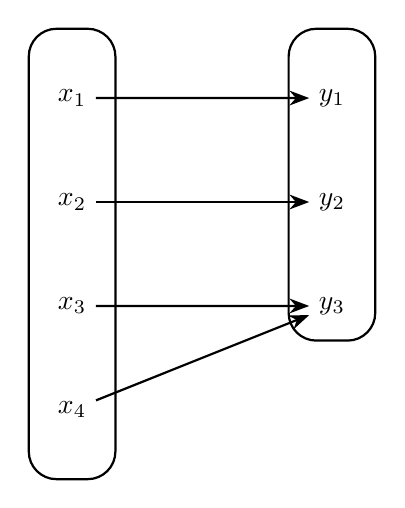
\begin{tikzpicture}[scale=1.1, every node/.style={scale=1}]


\draw[thick, rounded corners=10pt] (-0.5,-3.2) rectangle (0.5,2);


\draw[thick, rounded corners=10pt] (2.5,-1.6) rectangle (3.5,2);

\node (A1) at (0,1.2) {$x_1$};
\node (A2) at (0,0) {$x_2$};
\node (A3) at (0,-1.2) {$x_3$};
\node (A4) at (0,-2.4) {$x_4$};

\node (B1) at (3,1.2) {$y_1$};
\node (B2) at (3,0) {$y_2$};
\node (B3) at (3,-1.2) {$y_3$};

\draw[-{Stealth[length=2.5mm]}, thick] (A1) -- (B1);
\draw[-{Stealth[length=2.5mm]}, thick] (A2) -- (B2);
\draw[-{Stealth[length=2.5mm]}, thick] (A3) -- (B3);
\draw[-{Stealth[length=2.5mm]}, thick] (A4) -- (B3);
\end{tikzpicture}
}
\end{center}

\textbf{Example:}

\begin{enumerate}
\item $f : \mathbb{Z} \to \mathbb{N}$, where $f(x) = |x|$

   \[
   \begin{array}{c|ccccccc}
   x & -3 & -2 & -1 & 0 & 1 & 2 & 3 \\ \hline
   |x| & 3 & 2 & 1 & 0 & 1 & 2 & 3
   \end{array}
   \]

\item $f : \mathbb{R} \to \mathbb{R}$, where $f(x) = x^3$

   \[\forall y \in \mathbb{R}, \exists x = \sqrt[3]{y} \in \mathbb{R} \mid f(x) = y\]

\item $f : \mathbb{R} \to [0, \infty)$, where $f(x) = x^2$

   \[f(\sqrt{x}) = (\sqrt{x})^2 = x\]

\item Floor function: $f : \mathbb{R} \to \mathbb{Z}$, where $f(x) = \lfloor x \rfloor$

   \[
   \begin{array}{c|ccccc}
   x & -2.7 & -1.2 & 0.5 & 1.0 & 2.9 \\ \hline
   \lfloor x \rfloor & -3 & -2 & 0 & 1 & 2
   \end{array}
   \]
\end{enumerate}

\subsubsection{Bijective}

A function $f : A \rightarrow B$ is bijective if and only if it is both injective and surjective. We call such a function a bijection from $A$ to $B$, or a one-to-one correspondence.

Equivalently:

\[
\forall y \in B,\ \exists! x \in A \mid f(x) = y.
\]

(For every element in $B$, there exists exactly one element in $A$ that maps to it.)

\begin{center}
\fbox{
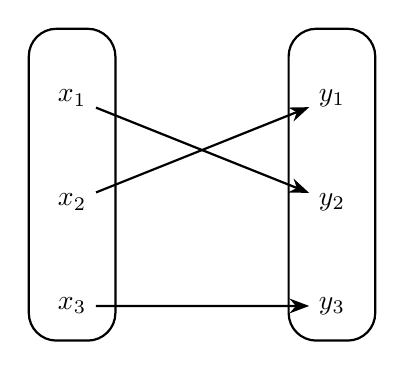
\begin{tikzpicture}[scale=1.1, every node/.style={scale=1}]


\draw[thick, rounded corners=10pt] (-0.5,-1.6) rectangle (0.5,2);


\draw[thick, rounded corners=10pt] (2.5,-1.6) rectangle (3.5,2);

\node (A1) at (0,1.2) {$x_1$};
\node (A2) at (0,0) {$x_2$};
\node (A3) at (0,-1.2) {$x_3$};

\node (B1) at (3,1.2) {$y_1$};
\node (B2) at (3,0) {$y_2$};
\node (B3) at (3,-1.2) {$y_3$};

\draw[-{Stealth[length=2.5mm]}, thick] (A1) -- (B2);
\draw[-{Stealth[length=2.5mm]}, thick] (A2) -- (B1);
\draw[-{Stealth[length=2.5mm]}, thick] (A3) -- (B3);
\end{tikzpicture}
}
\end{center}

\textbf{Example:}

Let
\[
A = \{1, 2, 3\}, \quad B = \{a, b, c\}.
\]

Define a function
\[
f : A \to B
\]
by
\[
f(1) = a, \quad f(2) = b, \quad f(3) = c.
\]

Each element of $A$ maps to a unique element of $B$, so $f$ is injective. Every element of $B$ is the image of some element of $A$, so $f$ is surjective. Therefore, $f$ is bijective.

\subsection{Combinations}

\subsubsection{Bijective (Both injective and surjective)}

\begin{enumerate}
\item Identity function: $f : \mathbb{R} \to \mathbb{R}$, where $f(x) = x$

   Injective and surjective, therefore bijective:
   \[\forall y \in \mathbb{R}, \exists! x \in \mathbb{R} \mid f(x) = y\]


\item $f : [0, \infty) \to [0, \infty)$, where $f(x) = x^2$

   Injective: \[\forall x_1, x_2 \in [0, \infty), x_1^2 = x_2^2 \Longrightarrow x_1 = x_2\]

   Surjective: \[\forall y \in [0, \infty), \exists x \in [0, \infty) \mid f(x) = y\]

   Therefore bijective.
\end{enumerate}

\subsubsection{Injective but not surjective}

Recall the Von Neumann Ordinal, 

\[\begin{aligned}
   0 &= \varnothing = \{\}\\
   1 &= \{\varnothing\} = \varnothing \cup \{\varnothing\}\\
   2 &= \{\varnothing, \{\varnothing\}\} = 1 \cup \{1\}\\
   &\vdots\\
   n &= n-1 \cup \{n-1\}
\end{aligned}
\]

Based on this notion, we can define a function that is injective but not surjective:

Let $A = \{1, 2, 3\}$ and define $f: A \to \mathcal{P}(A)$ by $f(x) = \{x\}$.

Then:
\[f(1) = \{1\}, \quad f(2) = \{2\}, \quad f(3) = \{3\}\]

Hence:
\[\operatorname{Im}(f) = \{\{1\}, \{2\}, \{3\}\} \subset \mathcal{P}(A)\]

Since $\varnothing \in \mathcal{P}(A)$ but $\varnothing \notin \operatorname{Im}(f)$, we conclude that $f$ is injective but not surjective.

\subsubsection{Surjective but not injective}

Piecewise function: $f : \mathbb{N} \to \mathbb{N}$, where
\[f(x) = \begin{cases} \frac{x}{2} & \text{if } x \text{ is even} \\[0.5em] \frac{x+1}{2} & \text{if } x \text{ is odd} \end{cases}\]

Surjective: \[\forall y \in \mathbb{N}, \exists x \in \mathbb{N} : f(x) = y\]

Not injective: \[f(1) = f(2) = 1 \text{ but } 1 \neq 2\]

\subsubsection{Neither injective nor surjective}

\begin{enumerate}
\item Constant function: $f : \mathbb{N} \to \mathbb{N}$, where $f(x) = 1$ for all $x$

   Not injective: \[f(1) = f(2) = 1 \text{ but } 1 \neq 2\]

   Not surjective: \[\nexists x \in \mathbb{N} \mid f(x) = 2\]

\item $f : \mathbb{R} \to \mathbb{R}$, where $f(x) = x^2$

   Not injective: \[f(-2) = f(2) = 4 \text{ but } -2 \neq 2\]

   Not surjective: \[\nexists x \in \mathbb{R} \mid f(x) = -1\]
\end{enumerate}

\subsection{Equivalence Relation with Function Properties}

Let $E = \{a, b, c, d, e, f\}$.

Define $R \subseteq E^2$:

\[
\begin{array}{c|cccccc}
R & a & b & c & d & e & f \\
\hline
a & (a,a) & (a,b) &  &  &  &  \\
b & (b,a) & (b,b) &  &  &  &  \\
c &  &  & (c,c) & (c,d) &  &  \\
d &  &  & (d,c) & (d,d) &  &  \\
e &  &  &  &  & (e,e) & (e,f) \\
f &  &  &  &  & (f,e) & (f,f) \\
\end{array}
\]
\newpage
By definition of equivalence:

\begin{enumerate}
\item Reflexive:
   \[
   \forall x \in E, \; (x,x) \in R
   \]

\item Symmetric:
   \[
   \forall x, y \in E, \; ((x,y) \in R \implies (y,x) \in R)
   \]

\item Transitive:
   \[
   \forall x, y, z \in E, \; ((x,y) \in R \wedge (y,z) \in R \implies (x,z) \in R)
   \]
\end{enumerate}

Equivalence Classes:

\[
\begin{aligned}
[a] &= \{a, b\} \\
[c] &= \{c, d\} \\
[e] &= \{e, f\}
\end{aligned}
\]

\[
E/R = \{[a], [c], [e]\}
\]

\begin{enumerate}
\item \textbf{Surjective function}

   \[
   f: E \to E/R, \quad f(x) = [x]
   \]

   \[
   \begin{aligned}
   f(a) &= [a], \quad f(b) = [a] \\
   f(c) &= [c], \quad f(d) = [c] \\
   f(e) &= [e], \quad f(f) = [e]
   \end{aligned}
   \]

   \begin{enumerate}
   \item Injective
   \[
   a \neq b \wedge f(a) = f(b) \implies \neg \text{Injective}
   \]

   \item Surjective
   \[
   \forall y \in E/R, \; \exists x \in E, \; f(x) = y \implies \text{Surjective}
   \]

   \item Bijective
   \[
   \neg \text{Injective} \implies \neg \text{Bijective}
   \]
   \end{enumerate}

   As a consequence, 

   \[
   E \not\cong E/R
   \]

\item \textbf{Bijective function}

   \[
   S = \{a, c, e\}, \text{ and } g: E/R \to S
   \]

   Then: 
   \[
   g([a]) = a, \quad g([c]) = c, \quad g([e]) = e
   \]

   \begin{enumerate}
   \item Injective
   \[
   \forall x_1, x_2 \in E/R, \; (g(x_1) = g(x_2) \implies x_1 = x_2) \implies \text{Injective}
   \]

   \item Surjective
   \[
   \forall y \in S, \; \exists x \in E/R, \; g(x) = y \implies \text{Surjective}
   \]

   \item Bijective
   \[
   \text{Injective} \wedge \text{Surjective} \implies \text{Bijective}
   \]
   \end{enumerate}

   We conclude that,

   \[
   E/R \cong S
   \]
\end{enumerate}


\section{Functions as Relations}

A function $f: A \to B$ defines a relation between $A$ and $B$:
\[
x \in A \text{ relates to } y \in B \iff f(x) = y
\]

We identify $f$ with its set of ordered pairs:
\[
f = \{(x, y) \mid x \in A \land f(x) = y\} \subseteq A \times B
\]

\subsection{Graph of a Function}

Let $R \subseteq A \times B$ satisfy:

\begin{enumerate}
\item If $xRy$ and $xRz$, then $y = z$; and
\item For every $x \in A$, there exists a $y \in B$ such that $\langle x, y \rangle \in R$.
\end{enumerate}

Then $R$ is the graph of a function $f : A \to B$ defined by $f(x) = y$ iff $xRy$.

Let $f : A \to B$ be a function. The graph of $f$ is the relation $R_f \subseteq A \times B$ defined by:

\[
R_f = \{ \langle x, y \rangle \mid f(x) = y \}.
\]

\textbf{Example:}

Define a function $f : \mathbb{N} \to \mathbb{Z}$ by
\[
f(n) = (-1)^n \cdot \left\lfloor \frac{n+1}{2} \right\rfloor
\]

Explicitly:
\[
\begin{aligned}
n = 0: & \quad \left\lfloor \frac{0+1}{2} \right\rfloor = \left\lfloor 0.5 \right\rfloor = 0 \implies f(0) = (-1)^0 \cdot 0 = 0 \\
n = 1: & \quad \left\lfloor \frac{1+1}{2} \right\rfloor = \left\lfloor 1 \right\rfloor = 1 \implies f(1) = (-1)^1 \cdot 1 = -1 \\
n = 2: & \quad \left\lfloor \frac{2+1}{2} \right\rfloor = \left\lfloor 1.5 \right\rfloor = 1 \implies f(2) = (-1)^2 \cdot 1 = 1 \\
n = 3: & \quad \left\lfloor \frac{3+1}{2} \right\rfloor = \left\lfloor 2 \right\rfloor = 2 \implies f(3) = (-1)^3 \cdot 2 = -2 \\
n = 4: & \quad \left\lfloor \frac{4+1}{2} \right\rfloor = \left\lfloor 2.5 \right\rfloor = 2 \implies f(4) = (-1)^4 \cdot 2 = 2
\end{aligned}
\]

Therefore: $f(0) = 0, \quad f(1) = -1, \quad f(2) = 1, \quad f(3) = -2, \quad f(4) = 2, \ldots$

Then the graph is:

\[R_f = \{(0,0), (1,-1), (2,1), (3,-2), (4,2), \ldots\}\]

Each element in $\mathbb{N}$ maps to exactly one element in $\mathbb{Z}$.

\subsection{Restriction and Image}

Let $f : A \to B$ be a function and $C \subseteq A$. The restriction of $f$ to $C$, denoted $f \upharpoonright C : C \to B$, is defined by:

\[
(f \upharpoonright C)(x) = f(x), \forall x \in C.
\]

Equivalently, as a graph:
\[
f \upharpoonright C = \{ \langle x, y \rangle \in R_f \mid x \in C \}.
\]

The image of $C$ under $f$ is:
\[
f[C] = \{ f(x) \mid x \in C \}.
\]

\textbf{Example:}

Let $f : \mathbb{N} \to \mathbb{Z}$ be as in the earlier example with $f(n) = (-1)^n \cdot \left\lfloor \displaystyle\frac{n+1}{2} \right\rfloor$

giving:
\[
f(0) = 0, \quad f(1) = -1, \quad f(2) = 1, \quad f(3) = -2, \quad f(5) = -3, \quad f(7) = -4, \ldots
\]

Let $C = \{2, 3, 5, 7, 11, 13, \ldots\}$. 

Then:

\[
\begin{aligned}
f \upharpoonright C &= \{(2, 1), (3, -2), (5, -3), (7, -4), (11, -6), (13, -7), \ldots\} \\
f[C] &= \{1, -2, -3, -4, -6, -7, \ldots\} = \{\text{images of all primes under } f\}
\end{aligned}
\]

The restriction $f \upharpoonright C$ is the subgraph where $x \in C$ (i.e., $x$ is prime), and the image $f[C]$ is the set of corresponding integer outputs.


\section{Inverse}

A function $g : Y \to X$ is an inverse of a function $f : X \to Y$ if
\[
f(g(y)) = y \quad \text{and} \quad g(f(x)) = x, \quad \forall x \in X, \forall y \in Y.
\]

\textbf{Example:}  
Let
\[
f(x) = a x + b, \qquad g(y) = \frac{y - b}{a}.
\]

Then we can verify that
\[
f(g(y)) = a \left( \frac{y - b}{a} \right) + b = y,
\]
and
\[
g(f(x)) = \frac{(a x + b) - b}{a} = x.
\]

Therefore, $g$ is the inverse of $f$.

\subsection{Left and Right Inverse}

Let $f : X \to Y$.

\begin{enumerate}
    \item A function $g : Y \to X$ is a \emph{left inverse} of $f$ if $g(f(x)) = x$, $\forall x \in X$.

    \textbf{Example:}  
    Let
    \[
    f: [0, \infty) \to \mathbb{R}, \quad f(x) = a^x, \ a > 0,\, a \neq 1.
    \]
    Define 
    \[
    g(y) = \log_a(y).
    \]
    Then
    \[
    g(f(x)) = \log_a(a^x) = x,
    \]
    so $g$ is a \emph{left inverse} of $f$.

    \item A function $h : Y \to X$ is a \emph{right inverse} of $f$ if $f(h(y)) = y$, $\forall y \in Y$.

    \textbf{Example:}  
    Let
    \[
    f: [0, \infty) \to \mathbb{R}, \quad f(x) = x^2.
    \]
    Define
    \[
    h(y) = \sqrt{y}.
    \]
    Then
    \[
    f(h(y)) = (\sqrt{y})^2 = y,
    \]
    so $h$ is a \emph{right inverse} of $f$.
\end{enumerate}

\textbf{Note:}

\begin{enumerate}
    \item \textbf{Left Inverse:}
    \[
    X \xrightarrow{\,f\,} Y \xrightarrow{\,g\,} X, \quad g(f(x)) = x, \forall x \in X.
    \]

    \item \textbf{Right Inverse:}
    \[
    Y \xrightarrow{\,h\,} X \xrightarrow{\,f\,} Y, \quad f(h(y)) = y, \forall y \in Y.
    \]

    \item \textbf{Two-Sided Inverse:}
    \[
    X \overset{f}{\underset{f^{-1}}{\longleftrightarrow}} Y, \quad f(f^{-1}(y)) = y, \quad f^{-1}(f(x)) = x.
    \]
\end{enumerate}

\subsection{Injective Case}

If $f : X \to Y$ is injective, then there exists a left inverse $g : Y \to X$ such that $g(f(x)) = x$, $\forall x \in X$.

\textbf{Proof:}

Suppose $f$ is injective. For each $y \in \operatorname{ran}(f)$, there exists a unique $x \in X$ such that $f(x) = y$. Define
\[
g(y) =
\begin{cases}
x & \text{if } f(x) = y \text{ for some } x \in X, \\
a & \text{otherwise, for fixed } a \in X.
\end{cases}
\]
Then $g$ is defined for all $y \in Y$, and for $y = f(x)$, we have $g(f(x)) = x$.

\textbf{Example 1:}

Let $X = \{1,2,3\}$ and $Y = \{a,b,c,d\}$. Define $f : X \to Y$ by
\[
f(1) = a, \quad f(2) = b, \quad f(3) = c.
\]
Then $f$ is injective but not surjective (since $d \notin \operatorname{ran}(f)$).

\textbf{Example 2:}

Define a function $g : Y \to X$ by
\[
g(a) = 1, \quad g(b) = 2, \quad g(c) = 3, \quad g(d) = 1.
\]

Then $\forall x \in X$, $g(f(x)) = x$, so $g$ is a left inverse of $f$.

\begin{center}
\fbox{
\begin{minipage}{0.45\textwidth}
\centering
\textbf{$f : X \to Y$}

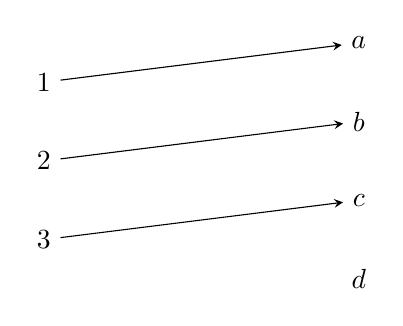
\begin{tikzpicture}[>=stealth, node distance=2cm]
% A nodes (left)
\node (A1) at (0,1) {1};
\node (A2) at (0,0) {2};
\node (A3) at (0,-1) {3};

% B nodes (right)
\node (B1) at (4,1.5) {$a$};
\node (B2) at (4,0.5) {$b$};
\node (B3) at (4,-0.5) {$c$};
\node (B4) at (4,-1.5) {$d$};

% f arrows
\draw[->] (A1) -- (B1);
\draw[->] (A2) -- (B2);
\draw[->] (A3) -- (B3);
\end{tikzpicture}
\end{minipage}
\hspace{0.05\textwidth}
\begin{minipage}{0.45\textwidth}
\centering
\textbf{$g : Y \to X$}

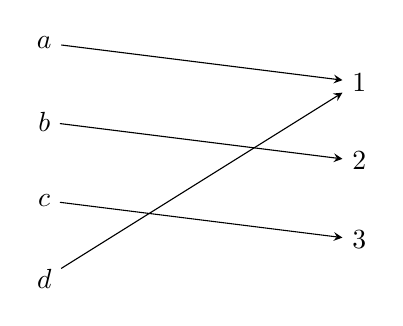
\begin{tikzpicture}[>=stealth, node distance=2cm]
% B nodes (left)
\node (B1) at (0,1.5) {$a$};
\node (B2) at (0,0.5) {$b$};
\node (B3) at (0,-0.5) {$c$};
\node (B4) at (0,-1.5) {$d$};

% A nodes (right)
\node (A1) at (4,1) {1};
\node (A2) at (4,0) {2};
\node (A3) at (4,-1) {3};

% g arrows
\draw[->] (B1) -- (A1);
\draw[->] (B2) -- (A2);
\draw[->] (B3) -- (A3);
\draw[->] (B4) -- (A1); % g(d) = 1 (arbitrary)
\end{tikzpicture}
\end{minipage}
}
\end{center}

\subsection{Surjective Case}

If $f : X \to Y$ is surjective, then there exists a right inverse $h : Y \to X$ such that $f(h(y)) = y$, $\forall y \in Y$.

\textbf{Example:}

Let $X = \{1,2,3,4\}$ and $Y = \{a,b\}$. Define $f : X \to Y$ by
\[
f(1) = a, \quad f(2) = b, \quad f(3) = a, \quad f(4) = b.
\]

Then $f$ is surjective but not injective.

A right inverse $h : Y \to X$ may be defined as
\[
h(a) = 1, \quad h(b) = 2.
\]

Then $\forall y \in Y$, $f(h(y)) = y$, so $h$ is a right inverse of $f$.

\begin{center}
\fbox{
\begin{minipage}{0.45\textwidth}
\centering
\textbf{$f : X \to Y$}

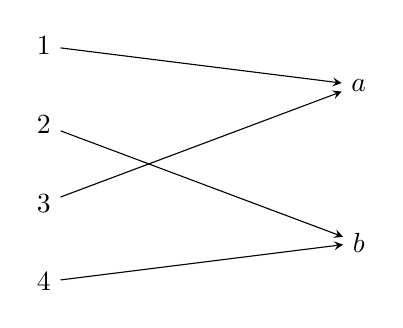
\begin{tikzpicture}[>=stealth, node distance=2cm]
% A nodes
\node (A1) at (0,1.5) {1};
\node (A2) at (0,0.5) {2};
\node (A3) at (0,-0.5) {3};
\node (A4) at (0,-1.5) {4};

% B nodes
\node (B1) at (4,1) {$a$};
\node (B2) at (4,-1) {$b$};

% Arrows for f
\draw[->] (A1) -- (B1);
\draw[->] (A3) -- (B1);
\draw[->] (A2) -- (B2);
\draw[->] (A4) -- (B2);
\end{tikzpicture}
\end{minipage}
\hspace{0.05\textwidth}
\begin{minipage}{0.45\textwidth}
\centering
\textbf{$h : Y \to X$}

\begin{tikzpicture}[>=stealth, node distance=2cm]
% B nodes (left)
\node (B1) at (0,1) {$a$};
\node (B2) at (0,-1) {$b$};

% A nodes (right)
\node (A1) at (4,1.5) {1};
\node (A2) at (4,0.5) {2};
\node (A3) at (4,-0.5) {3};
\node (A4) at (4,-1.5) {4};

% Arrows for h
\draw[->] (B1) -- (A1);
\draw[->] (B2) -- (A2);
\end{tikzpicture}
\end{minipage}
}
\end{center}.

\subsection{Bijective Case}

If $f : X \to Y$ is bijective, then there exists a function $f^{-1} : Y \to X$ such that
\[
f^{-1}(f(x)) = x, \forall x \in X, \quad \text{and} \quad f(f^{-1}(y)) = y, \forall y \in Y.
\]

\textbf{Example:}

Let $X = \{1,2,3\}$ and $Y = \{a,b,c\}$ with
\[
f(1) = a, \quad f(2) = b, \quad f(3) = c.
\]

Then $f$ is bijective. Its inverse $f^{-1}$ satisfies
\[
f^{-1}(a) = 1, \quad f^{-1}(b) = 2, \quad f^{-1}(c) = 3.
\]
\begin{center}
\fbox{
\begin{minipage}{0.45\textwidth}
\centering
\textbf{$f : X \to Y$}

\begin{tikzpicture}[>=stealth, node distance=2cm]
% A nodes
\node (A1) at (0,1) {1};
\node (A2) at (0,0) {2};
\node (A3) at (0,-1) {3};

% B nodes
\node (B1) at (4,1) {$a$};
\node (B2) at (4,0) {$b$};
\node (B3) at (4,-1) {$c$};

% Arrows for f
\draw[->] (A1) -- (B1);
\draw[->] (A2) -- (B2);
\draw[->] (A3) -- (B3);
\end{tikzpicture}
\end{minipage}
\hspace{0.05\textwidth}
\begin{minipage}{0.45\textwidth}
\centering
\textbf{$f^{-1} : Y \to X$}

\begin{tikzpicture}[>=stealth, node distance=2cm]
% B nodes
\node (B1) at (0,1) {$a$};
\node (B2) at (0,0) {$b$};
\node (B3) at (0,-1) {$c$};

% A nodes
\node (A1) at (4,1) {1};
\node (A2) at (4,0) {2};
\node (A3) at (4,-1) {3};

% Arrows for f^{-1}
\draw[->] (B1) -- (A1);
\draw[->] (B2) -- (A2);
\draw[->] (B3) -- (A3);
\end{tikzpicture}
\end{minipage}
}
\end{center}

\subsection{Uniqueness of Inverse}

If $f : X \to Y$ has a left inverse $g$ and a right inverse $h$, then $g = h$. Hence, every function has at most one inverse.

\textbf{Example 1:}

Let  
\[
X = \{1, 2, 3\}, \quad Y = \{a, b, c\}.
\]

Define  
\[
f : X \to Y, \quad f(1) = a, \; f(2) = b, \; f(3) = c.
\]

Then $f$ is bijective.

Let  
\[
g : Y \to X, \quad g(a) = 1, \; g(b) = 2, \; g(c) = 3,
\]
and  
\[
h : Y \to X, \quad h(a) = 1, \; h(b) = 2, \; h(c) = 3.
\]

Then  
\[
g(f(x)) = x \quad \text{and} \quad f(h(y)) = y.
\]

Thus $g$ is a left inverse, $h$ is a right inverse, and  
\[
g = h = f^{-1}.
\]

Hence, the inverse of $f$ is unique.

\textbf{Example 2:} 

Let  
\[
f : \mathbb{N} \to \mathbb{Q}, \quad f(n) = n,
\]
where we regard $\mathbb{N} \subset \mathbb{Q}$. Then $f$ is injective but not surjective, since many rational numbers (e.g., $\frac{1}{2}, \frac{3}{4}$) are not images of any natural number.

Define  
\[
g : \mathbb{Q} \to \mathbb{N}, \quad
g(q) = 
\begin{cases}
n, & \text{if } q = n \in \mathbb{N}, \\
1, & \text{otherwise}.
\end{cases}
\]

Then $\forall n \in \mathbb{N}$,  
\[
g(f(n)) = g(n) = n,
\]
so $g$ is a left inverse of $f$.

However, $f$ has no right inverse, since it is not surjective; there is no $h : \mathbb{Q} \to \mathbb{N}$ such that  
\[
f(h(q)) = q, \forall q \in \mathbb{Q}.
\]

Hence, $f$ has a left inverse but no right inverse, and therefore no true inverse. If a true inverse existed, it would be unique.


% ===== PART 26 =====%
\section{Truth Value for FOL}

In propositional logic (PL), every atomic sentence is directly assigned
a truth value (true or false). On the other hand, in first-order logic
(FOL), the truth value of a predicate is determined relative to an
interpretation and a variable assignment.

For example:

Let domain \(D = \{1,2,3\}\), for \(E(x)\) = ``\(x\) is even''.

Hence:

\begin{enumerate}
  \item \(E(1) =\) False
  \item \(E(2) =\) True
  \item \(E(3) =\) False
\end{enumerate}


\subsection{Example 1}\label{example-1}

Let the domain: \[D = \{\langle x,y \rangle \in \mathbb{N}^2\}\]

Evaluate: \[\forall x,y  \in D \;(x \cdot y > x + y)\]

However, by antisymmetric schema, we can find a counterexample:

\[
\exists x \exists y \;\big((\langle x, y \rangle \in \mathbb{N}^2) \;\land\; x = y \;\land\; x = 2 \;\land\; y = 2 \;\land\; (x \cdot y = x + y) \;\land\; \neg(x \cdot y > x + y)\big)
\]

Therefore: \[\boxed{\neg \forall x,y \in D \;(x \cdot y > x + y)}\]

Note that other counterexamples include \(\langle 1,1 \rangle\),
\(\langle 1,2 \rangle\), \(\langle 2,1 \rangle\), and
\(\langle 1,n \rangle\) for any \(n \in \mathbb{N}\).

\subsection{Example 2}\label{example-2}

Let the domain: \[D = \mathbb{Z}\]

Evaluate:

\[\forall x \forall y \forall z \;(x, y, z \in \mathbb{Z} \to ((x + y = z) \to z > 0))\]

However, we can find a counterexample:

\[\exists x \exists y \exists z \;(x, y, z \in \mathbb{Z} \;\land\; x = -1 \;\land\; y = -2 \;\land\; z = -3 \;\land\; (x + y = z) \;\land\; \neg(z > 0))\]

Since \(-3 \not> 0\), we have shown that there exist integers where the
sum equals \(z\) but \(z\) is not positive.

Consequently:

\[\boxed{\neg \forall x \forall y \forall z \;((x + y = z) \to z > 0)}\]

\subsection{Example 3}\label{example-3}

Let the domain:

\[
D = \displaystyle\left\{ x \in \mathbb{Z} \;\middle|\; \frac{3x}{2} + 1 + \frac{4x}{3} = -\frac{31}{8} + \frac{2x}{3} \right\}.
\]

Evaluate:

\[
\exists x \,(x \in D).
\]

Since \(-\tfrac{9}{4} \notin \mathbb{Z}\),

Thus:

\[
\boxed{D = \varnothing}
\]

And the statement is false, because the domain is empty.

\subsection{Example 4}\label{example-4}

Let the domain:
\[D = \{\langle x,y \rangle \in \mathbb{R}^2 \mid x + 2y = 16\} \]

Evaluate:

\[ \forall  x, y \in D \, ((x \in \mathbb{R} \land y \in \mathbb{Z}) \to x > y) \]

Since we can find a counterexample:

\[\exists x \exists y \;(x \in \mathbb{R} \;\land\; y \in \mathbb{Z} \;\land\; x = 0 \;\land\; y = 8 \;\land\; (x + 2y = 16) \;\land\; \neg(x > y))\]

Therefore:

\[\boxed{\neg \forall x, y \in D \, ((x \in \mathbb{R} \land y \in \mathbb{Z}) \to x > y)}\]

\subsection{Example 5}\label{example-5}

Let the domain: \[D = \{\langle x,y \rangle \in \mathbb{Z}^2\}\]

Evaluate:
\[\forall \langle x,y \rangle \in D \;(\text{even}(x) \leftrightarrow \text{even}(y))\]

However, we can find a counterexample:

\[
\exists x \exists y \;\big((\langle x, y \rangle \in \mathbb{Z}^2) \;\land\; x = 4 \;\land\; y = 3 \;\land\; \text{even}(x) \;\land\; \neg\text{even}(y) \;\land\; \neg(\text{even}(x) \leftrightarrow \text{even}(y))\big)
\]

Therefore:

\[\boxed{\neg \forall \langle x,y \rangle \in D \;(\text{even}(x) \leftrightarrow \text{even}(y))}\]

Note that other counterexamples include \(\langle 2,5 \rangle\),
\(\langle 7,8 \rangle\), and any pair where one number is even and the
other is odd.


% ===== PART 25 =====%

\section{Natural Deduction for FOL}


\subsection{Universal Elimination ($\forall$E)}\label{sec:universal-elimination}

\[
\begin{nd}
  \hypo {1} {\forall x.P(x)}
  \have {2} {P(a)}                       \Ae{1}
  \have {3} {P(b)}                       \Ae{1}
\end{nd}
\]


\subsection{Universal Introduction ($\forall$I)}\label{sec:universal-introduction}

\[
\begin{nd}
  \hypo {1} {P(a)}
  \have {2} {P(a) \lor Q(a)}             \Ai{1}
  \close
  \have {3} {\forall x.(P(x) \lor Q(x))} \Ai{1-2}
\end{nd}
\]

\subsection{Existential Introduction ($\exists$I)}\label{sec:existential-introduction}

\[
\begin{nd}
  \hypo {1} {P(a)}
  \have {2} {\exists x.P(x)}             \Ei{1}
  \have {3} {\exists x.(P(x) \land Q(a))} \Ei{1}
\end{nd}
\]

\subsection{Existential Elimination ($\exists$E)}\label{sec:existential-elimination}

\[
\begin{nd}
  \hypo {1} {\exists x.P(x)}
  \hypo {2} {\forall x.(P(x) \to Q(x))}
  \open[a]
  \hypo {3} {P(a)}
  \have {4} {P(a) \to Q(a)}              \Ae{2}
  \have {5} {Q(a)}                       \ie{3,4}
  \close
  \have {6} {Q(a)}                       \Ee{1,3-5}
  \have {7} {\exists x.Q(x)}             \Ei{6}
\end{nd}
\]

\subsection{Identity Introduction ($=$I)}\label{sec:identity-introduction}
\[
\begin{nd}
  \hypo {1} {P(a)}
  \have {2} {Q(a) \to R(a)}              \by{...}{}
  \have {3} {S(a)}                       \by{...}{}
  \have {n} {a = a}                      \by{=I}{}
\end{nd}
\]

\subsection{Identity Elimination ($=$E)}\label{sec:identity-elimination}

\[
\begin{nd}
  \hypo {1} {a = b}
  \hypo {2} {P(a)}
  \have {3} {P(b)}                       \by{=E}{1,2}
\end{nd}
\]

% ===== PART 26 =====%
\section{Boolean, DNF, and CNF}

\subsection{Boolean}\label{boolean}

In short, the application of Boolean Algebra is essentially the same as
Formal Logic. The main difference lies in the symbols used. For example,
in Formal Logic, the symbol $\land$ is used for logical AND, whereas
in Boolean Algebra we often use $\,\cdot\,$ (dot) for AND. Logical OR,
represented by $\lor$ in Formal Logic, corresponds to $+$ in Boolean
Algebra. Negation, $\neg x$ in Formal Logic, is written as $\bar{x}$
in Boolean Algebra. Sometimes, you may also encounter the AND and OR
symbols inside circles: $\oplus$ for XOR (exclusive OR) and $\odot$
or $\otimes$ for AND, depending on the text. These are just
alternative notations and do not change the underlying logic.

Furthermore, it is important to note that Boolean Algebra is not the
same as conventional mathematics. Specifically, Boolean Algebra operates
strictly on binary values ($1$ and $0$). General mathematics
typically deals with a wider range of numbers, including integers,
fractions, and complex numbers.

\begin{center}
\begin{tabular}{|p{0.45\linewidth}|p{0.50\linewidth}|}
\hline
\textbf{Property} & \textbf{Expression} \\
\hline
Binary Operation $+$ & $1 + 0 = 1$ \\
\hline
Commutative Property of $+$ & $1 + 0 = 0 + 1$ \\
\hline
Associative Property of $+$ & $(1 + 0) + 1 = 1 + (0 + 1)$ \\
\hline
Binary Operation $\cdot$ & $1 \cdot 1 = 1$ \\
\hline
Commutative Property of $\cdot$ & $1 \cdot 0 = 0 \cdot 1$ \\
\hline
Associative Property of $\cdot$ & $(1 \cdot 0) \cdot 1 = 1 \cdot (0 \cdot 1)$ \\
\hline
Distributive Properties & $1 \cdot (0 + 1) = (1 \cdot 0) + (1 \cdot 1)$ \\
\hline
Special Combinations & $a = a \cdot (a + b)$ \\
\hline
Unary Operation $\bar{}$ (Negation) & $\bar{1} = 0, \bar{0} = 1$ \\
\hline
Identity with $+$ & $a + 0 = a$ \\
\hline
Annihilation with $\cdot$ & $a \cdot 0 = 0$ \\
\hline
Proof using Commutativity of $+$ & $a + b = b + a$ \\
\hline
Proof using Commutativity of $\cdot$ & $a \cdot b = b \cdot a$ \\
\hline
Identity Property of $+$ & $a + 0 = a$ \\
\hline
Zero for $+$ & $0 + a = a$ \\
\hline
Commutative Property for Zero & $0 + a = a + 0$ \\
\hline
Identity with $\cdot$ & $a \cdot 1 = a$ \\
\hline
Idempotent Law for $+$ & $a + a = a$ \\
\hline
Idempotent Law for $\cdot$ & $a \cdot a = a$ \\
\hline
Annihilation with $+$ & $a + 1 = 1$ \\
\hline
Annihilation with $\cdot$ & $a \cdot 0 = 0$ \\
\hline
Double Negation & $\overline{\overline{a}} = a$ \\
\hline
De Morgan's Law for $+$ & $\overline{a \cdot b} = \bar{a} + \bar{b}$ \\
\hline
De Morgan's Law for $\cdot$ & $\overline{a + b} = \bar{a} \cdot \bar{b}$ \\
\hline
\end{tabular}
\end{center}

Let $k \geq 1$. A $k$-ary Boolean function $f$ takes as input
$k$ True/False values and outputs a True/False value; namely, it is a
mapping.

$$f : \{1, 0\}^k \to \{1, 0\}$$

\textbf{Example:}

$$f_{p_1 \cdot p_2}(x_1, x_2) = \begin{cases} 1 & \text{if } x_1 \text{ and } x_2 \text{ both equal } 1 \\ 0 & \text{otherwise} \end{cases}$$

Let $k \geq 1$ and let $A$ be a propositional formula that uses (at
most) the variables $p_1, \ldots, p_k$. The $k$-ary Boolean function
$f_A(x_1, x_2, \ldots, x_k)$ is defined by

$$f_A(x_1, \ldots, x_k) = \varphi(A), \text{ where } \varphi(p_i) = x_i \text{ for } i = 1, 2, \ldots, k$$

Construction:

$$f(x_1, x_2) = \begin{cases} 1 & \text{if } x_1 = 1 \text{ or } x_2 = 0 \\ 0 & \text{otherwise} \end{cases}$$

\begin{center}
\begin{tabular}{|l|l|l|}
\hline
$x_1$ & $x_2$ & $f(x_1, x_2)$ \\
\hline
$1$ & $1$ & $1$ \\
\hline
$1$ & $0$ & $1$ \\
\hline
$0$ & $1$ & $0$ \\
\hline
$0$ & $0$ & $1$ \\
\hline
\end{tabular}
\end{center}

$$(p_1 \cdot p_2) + (p_1 \cdot \bar p_2) + (\bar p_1 \cdot \bar p_2)$$

\subsubsection{General Construction}

For $1 \leq i \leq 2^k$ and $1 \leq j \leq k$:

Form Disjunctions (Clauses):

$$\psi_i = \displaystyle\bigvee_{j=1}^k L_{i,j} := L_{i,1} + L_{i,2} + \cdots + L_{i,k}$$

Form Conjunctions (Clauses):

$$\Sigma_i = \displaystyle\bigwedge_{j=1}^k L_{i,j} := L_{i,1} \cdot L_{i,2} \cdot \cdots \cdot L_{i,k}$$

\textbf{Example:}

Let's take two propositional variables:
$$p_1, p_2$$

Possible truth assignments:

\begin{center}
\begin{tabular}{|l|c|c|}
\hline
$i$ & $p_1$ & $p_2$ \\
\hline
1 & 1 & 1 \\
\hline
2 & 1 & 0 \\
\hline
3 & 0 & 1 \\
\hline
4 & 0 & 0 \\
\hline
\end{tabular}
\end{center}

For each row $i$, we will form literals $L_{i,1}$ and $L_{i,2}$:
\begin{enumerate}
\item If $\varphi_i(p_j) = 1$, then $L_{i,j} = p_j$ 
\item If $\varphi_i(p_j) = 0$, then $L_{i,j} = \bar p_j$
\end{enumerate}

Conjunction:

$$C_i = L_{i,1} \cdot L_{i,2}$$

\begin{center}
\begin{tabular}{|l|c|l|}
\hline
$i$ & $(p_1, p_2)$ & $C_i$ \\
\hline
1 & (1, 1) & $p_1 \cdot p_2$ \\
\hline
2 & (1, 0) & $p_1 \cdot \bar p_2$ \\
\hline
3 & (0, 1) & $\bar p_1 \cdot p_2$ \\
\hline
4 & (0, 0) & $\bar p_1 \cdot \bar p_2$ \\
\hline
\end{tabular}
\end{center}

Each $C_i$ corresponds to \emph{one minterm}, True for exactly one
assignment.

Disjunction:

$$D_i = L_{i,1} + L_{i,2}$$

\begin{center}
\begin{tabular}{|l|c|l|}
\hline
$i$ & $(p_1, p_2)$ & $D_i$ \\
\hline
1 & (1, 1) & $p_1 + p_2$ \\
\hline
2 & (1, 0) & $p_1 + \bar p_2$ \\
\hline
3 & (0, 1) & $\bar p_1 + p_2$ \\
\hline
4 & (0, 0) & $\bar p_1 + \bar p_2$ \\
\hline
\end{tabular}
\end{center}

Each $D_i$ corresponds to \emph{one maxterm}, False for exactly one
assignment.

\subsection{Disjunctive Normal Form (DNF)}

The idea of DNF is that we can reduce all connectives in propositional
logic (PL) to only $+ \ \text{(Disjunction)}$,
$.\ \text{(Conjunction)}$, and $\bar x ~\text{(negation)}$ in order
to determine the truth value of a sentence.

\textbf{Example:}

$$(s \cdot a) + (\bar m \cdot b) + (\bar h \cdot \bar l) + (r \cdot \bar i)$$

Moreover, for convenience we use $(\pm L)$ to indicate that $L$ is
an atomic sentence which may or may not be prefaced with an occurrence
of negation. DNF example:

$$(\pm L_1 \cdot \dots \cdot \pm L_{i+1}) + (\pm L_j \cdot \dots \cdot \pm L_{k+1})$$

In detail:

Let $L$ be a sentence containing three atomic sentences $a, b, c$.

\begin{center}
\begin{tabular}{|c|c|c|c|}
\hline
$a$ & $b$ & $c$ & $L$ \\
\hline
1 & 1 & 1 & 1 \\
\hline
1 & 1 & 0 & 0 \\
\hline
1 & 0 & 1 & 1 \\
\hline
1 & 0 & 0 & 0 \\
\hline
0 & 1 & 1 & 0 \\
\hline
0 & 1 & 0 & 0 \\
\hline
0 & 0 & 1 & 1 \\
\hline
0 & 0 & 0 & 1 \\
\hline
\end{tabular}
\end{center}

From the truth table, we observe that $L$ is true on lines
$1, 3, 7, 8$. For each of these lines, we construct a conjunction that
captures the exact truth value assignment on that line:

\begin{enumerate}
\item Line 1: $(a \cdot b \cdot c)$
\item Line 3: $(a \cdot \bar b \cdot c)$
\item Line 7: $(\bar a \cdot \bar b \cdot c)$
\item Line 8: $(\bar a \cdot \bar b \cdot \bar c)$
\end{enumerate}

Therefore, a DNF representation logically equivalent to $L$ is:

$$(a \cdot b \cdot c) + (a \cdot \bar b \cdot c) + (\bar a \cdot \bar b \cdot c) + (\bar a \cdot \bar b \cdot \bar c)$$

This gives us a sentence in DNF which is true on exactly those lines
where one of the disjuncts is true, namely, lines 1, 3, 7, and 8. Hence,
the DNF sentence has exactly the same truth table as $L$. In other
words, we have produced a sentence in DNF that is logically equivalent
to $L$, which is precisely the goal of normalization.

\subsubsection{General Construction}

Let $L$ be a sentence containing atomic sentences $x_1, \dots, x_n$.
We aim to construct a new sentence, $G$, that is \emph{logically
equivalent} to $L$ but written in DNF. Intuitively, $G$ will serve
as a \emph{truth-functional reconstruction} of $L$: it will reproduce
the truth value of $L$ on every possible assignment of truth values to
$x_1, \dots, x_n$. That is, for each possible line of the truth table
for $L$, $G$ will be true if and only if $L$ is true on that line.
Hence, $G$ acts as the DNF counterpart of $L$, the formula that
expresses $L$'s truth behavior in canonical disjunctive form.

\begin{center}
\begin{tabular}{|c|c|c|c|c|c|}
\hline
Line & $x_1$ & $x_2$ & $\dots$ & $x_n$ & $L$ \\
\hline
1 & 1 & 1 & $\dots$ & 1 & $L_1$ \\
\hline
2 & 1 & 1 & $\dots$ & 0 & $L_2$ \\
\hline
3 & 1 & 0 & $\dots$ & 1 & $L_3$ \\
\hline
$\vdots$ & $\vdots$ & $\vdots$ & $\vdots$ & $\vdots$ & $\vdots$ \\
\hline
$2^n$ & 0 & 0 & $\dots$ & 0 & $L_{2^n}$ \\
\hline
\end{tabular}
\end{center}

Case 1:

If $L$ is false on every line of its truth table, then $L$ is a
contradiction. In that case, a contradiction of the form is in DNF and
is logically equivalent to $L$.

Case 2:

If $L$ is true on at least one line of its truth table, we proceed as
follows. For each line $i$ where $L = 1$, let $\psi_i$ be a
conjunction of the form:

$$\psi_i = \displaystyle\bigwedge_{m=1}^{n} (\pm x_m)$$

where

$$
(\pm x_m) =
\begin{cases}
x_m, & \text{if } x_m = 1 \text{ on line } i, \\
\bar x_m, & \text{if } x_m = 0 \text{ on line } i.
\end{cases}
$$

That is, $x_m$ appears unnegated in $\psi_i$ if it is true on line
$i$, and negated if it is false on line $i$. Thus, $\psi_i$ is
true on, and only on, line $i$ of the truth table.

Now, let $i_1, i_2, \dots, i_j$ be the indices of all lines where
$L = 1$. Then we define $G$ as the disjunction of all such
$\psi_i$:

$$G = \psi_{i_1} + \psi_{i_2} + \dots + \psi_{i_j} = \displaystyle\bigvee_{k=1}^{j} \left[ \bigwedge_{m=1}^{n} (\pm x_m) \right]$$

Since $G$ is a disjunction of conjunctions of literals, $G$ is in
DNF. By construction, $L$ and $G$ are true on exactly the same lines
of the truth table, and therefore

$$L \equiv G$$

\textbf{Example:}

Let $S$ contain three atomic sentences $x_1, x_2, x_3$.

\begin{center}
\begin{tabular}{|c|c|c|c|}
\hline
$x_1$ & $x_2$ & $x_3$ & $S$ \\
\hline
1 & 1 & 1 & 1 \\
\hline
1 & 1 & 0 & 0 \\
\hline
1 & 0 & 1 & 1 \\
\hline
1 & 0 & 0 & 0 \\
\hline
0 & 1 & 1 & 0 \\
\hline
0 & 1 & 0 & 0 \\
\hline
0 & 0 & 1 & 1 \\
\hline
0 & 0 & 0 & 1 \\
\hline
\end{tabular}
\end{center}

$S = 1$ on lines 1, 3, 7, and 8.

\begin{enumerate}
\item For line 1: $f_1 = (x_1 \cdot x_2 \cdot x_3)$
\item For line 3: $f_3 = (x_1 \cdot \bar x_2 \cdot x_3)$
\item For line 7: $f_7 = (\bar x_1 \cdot \bar x_2 \cdot x_3)$
\item For line 8: $f_8 = (\bar x_1 \cdot \bar x_2 \cdot \bar x_3)$
\end{enumerate}

Form the disjunction: 
$$B = f_1 + f_3 + f_7 + f_8$$

Hence,

$$\big[(x_1 \cdot x_2 \cdot x_3) + (x_1 \cdot \bar x_2 \cdot x_3) + (\bar x_1 \cdot \bar x_2 \cdot x_3) + (\bar x_1 \cdot \bar x_2 \cdot \bar x_3)\big]$$

We conclude that, 
$$S \equiv B$$

\subsection{Conjunctive Normal Form (CNF)}

Shortly, the formal definition of CNF is also analogous to the
definition of DNF.

\textbf{Example:}

$$(s + a) \cdot (\bar m + b) \cdot (\bar h + \bar l) \cdot (r + \bar i)$$

and

$$(\pm T_1 + \dots + \pm P_m) \cdot (\pm T_i + \dots + \pm T_k)$$

In detail:

Consider a sentence $T$ with atomic sentences $p, q, r$.

\begin{center}
\begin{tabular}{|c|c|c|c|}
\hline
$p$ & $q$ & $r$ & $B$ \\
\hline
1 & 1 & 1 & 1 \\
\hline
1 & 1 & 0 & 0 \\
\hline
1 & 0 & 1 & 1 \\
\hline
1 & 0 & 0 & 0 \\
\hline
0 & 1 & 1 & 1 \\
\hline
0 & 1 & 0 & 0 \\
\hline
0 & 0 & 1 & 1 \\
\hline
0 & 0 & 0 & 1 \\
\hline
\end{tabular}
\end{center}

The truth table shows $T$ is false on lines $2, 4, 6$. We build a
clause for each false row by taking the disjunction of literals that
would make that row true:

\begin{enumerate}
\item Line 2: $(\bar p + \bar q + r)$
\item Line 4: $(\bar p + q + r)$
\item Line 6: $(p + \bar q + r)$
\end{enumerate}

A CNF formula logically equivalent to $T$:

$$(\bar p + \bar q + r) \cdot (\bar p + q + r) \cdot (p + \bar q + r)$$

Each clause eliminates exactly one false row. The conjunction ensures
all three clauses hold simultaneously, making the formula false
precisely where $M$ is false and true elsewhere.

\subsubsection{General Construction}

Given sentence $L$ with atomic sentences $y_1, \dots, y_n$, we
construct an equivalent sentence $H$ in CNF. The strategy: identify
where $L$ fails and build clauses that fail at exactly those points.

\begin{center}
\begin{tabular}{|c|c|c|c|c|c|}
\hline
Line & $y_1$ & $y_2$ & $\dots$ & $y_n$ & $L$ \\
\hline
1 & 1 & 1 & $\dots$ & 1 & $L_1$ \\
\hline
2 & 1 & 1 & $\dots$ & 0 & $L_2$ \\
\hline
3 & 1 & 0 & $\dots$ & 1 & $L_3$ \\
\hline
$\vdots$ & $\vdots$ & $\vdots$ & $\vdots$ & $\vdots$ & $\vdots$ \\
\hline
$2^n$ & 0 & 0 & $\dots$ & 0 & $L_{2^n}$ \\
\hline
\end{tabular}
\end{center}

Case 1:

When $L$ is true everywhere, it is a tautology. Any tautological
formula in CNF serves as an equivalent, such as $(p + \bar{p})$ or any
logically equivalent tautology.

Case 2:

When $L$ is false on some lines, for each line $j$ where $L = 0$,
construct clause $\phi_j$:

$$\phi_j = \displaystyle\bigvee_{t=1}^{n} (\pm y_t)$$

where

$$
(\pm y_t) =
\begin{cases}
\bar y_t, & \text{if } y_t = 1 \text{ on line } j, \\
y_t, & \text{if } y_t = 0 \text{ on line } j.
\end{cases}
$$

Each literal is the opposite of its truth value on line $j$, making
$\phi_j$ false only on line $j$.

Let $j_1, j_2, \dots, j_s$ index all lines where $L = 0$. Define:

$$H = \phi_{j_1} \cdot \phi_{j_2} \cdot \dots \cdot \phi_{j_s} = \displaystyle\bigwedge_{w=1}^{s} \left[ \bigvee_{t=1}^{n} (\pm y_t) \right]$$

$H$ is in CNF. Since $H$ is false exactly where $L$ is false:

$$L \equiv H$$

\textbf{Example:}

Let $R$ have atomic sentences $y_1, y_2, y_3$.

\begin{center}
\begin{tabular}{|c|c|c|c|}
\hline
$y_1$ & $y_2$ & $y_3$ & $R$ \\
\hline
1 & 1 & 1 & 1 \\
\hline
1 & 1 & 0 & 0 \\
\hline
1 & 0 & 1 & 1 \\
\hline
1 & 0 & 0 & 1 \\
\hline
0 & 1 & 1 & 0 \\
\hline
0 & 1 & 0 & 1 \\
\hline
0 & 0 & 1 & 0 \\
\hline
0 & 0 & 0 & 1 \\
\hline
\end{tabular}
\end{center}

$R = 0$ on lines 2, 5, and 7.

\begin{enumerate}
\item For line 2: $g_2 = (\bar y_1 + \bar y_2 + y_3)$
\item For line 5: $g_5 = (y_1 + \bar y_2 + \bar y_3)$
\item For line 7: $g_7 = (y_1 + y_2 + \bar y_3)$
\end{enumerate}

Form the conjunction: 
$$C = g_2 \cdot g_5 \cdot g_7$$

Hence,

$$\big[(\bar y_1 + \bar y_2 + y_3) \cdot (y_1 + \bar y_2 + \bar y_3) \cdot (y_1 + y_2 + \bar y_3)\big]$$

We conclude that, 
$$R \equiv C$$

\newpage

\textbf{Example 1:}

Let

$$\Sigma = a \to \bar b$$

First, we rewrite using the definition of implication:

$$\Sigma = (a \to \bar b \equiv \bar a + \bar b)$$

Truth Table: 

\begin{center}
\begin{tabular}{|c|c|c|c|c|}
\hline
$a$ & $b$ & $\bar a$ & $\bar b$ & $\Sigma$ \\
\hline
1 & 1 & 0 & 0 & 0 \\
\hline
1 & 0 & 0 & 1 & 1 \\
\hline
0 & 1 & 1 & 0 & 1 \\
\hline
0 & 0 & 1 & 1 & 1 \\
\hline
\end{tabular}
\end{center}

Hence,

\begin{enumerate}
\item DNF Construction:

  \begin{enumerate}
  \item Line 2: $(a \cdot \bar b)$
  \item Line 3: $(\bar a \cdot b)$
  \item Line 4: $(\bar a \cdot \bar b)$
  \end{enumerate}

  Therefore,

  $$\Sigma= (a \cdot \bar b) + (\bar a \cdot b) + (\bar a \cdot \bar b)$$
\item CNF Construction:

  \begin{enumerate}
  \item Line 1: $(\bar a + \bar b)$
  \end{enumerate}

  Thus,

  $$\Sigma= (\bar a + \bar b)$$
\item Both forms are logically equivalent:

  $$\Sigma \equiv \bar a + \bar b$$
\end{enumerate}

\textbf{Example 2:}

Let

$$\gamma = \neg(p \equiv q)$$

First, we rewrite using the definition of biconditional:

$$p \leftrightarrow q \equiv (p \cdot q) + (\bar{p} \cdot \bar{q})$$

Then, applying negation:

$$
\neg(p \leftrightarrow q) \equiv \neg[(p \cdot q) + (\bar{p} \cdot \bar{q})]
$$

Using De Morgan's law:

$$
\gamma = (\bar{p} + \bar{q}) \cdot (p + q)
$$

Truth Table: 

\begin{center}
\begin{tabular}{|c|c|c|c|c|c|}
\hline
$p$ & $q$ & $\bar p$ & $\bar q$ & $p \equiv q$ & $\gamma$ \\
\hline
1 & 1 & 0 & 0 & 1 & 0 \\
\hline
1 & 0 & 0 & 1 & 0 & 1 \\
\hline
0 & 1 & 1 & 0 & 0 & 1 \\
\hline
0 & 0 & 1 & 1 & 1 & 0 \\
\hline
\end{tabular}
\end{center}

\begin{enumerate}
\item DNF Construction

  $\gamma = 1$ on lines 2 and 3.

  \begin{enumerate}
  \item Line 2: $(p \cdot \bar{q})$
  \item Line 3: $(\bar{p} \cdot q)$
  \end{enumerate}

  Therefore,

  $$
   \gamma = (p \cdot \bar{q}) + (\bar{p} \cdot q)
   $$
\item CNF Construction

  $\gamma = 0$ on lines 1 and 4.

  \begin{enumerate}
  \item Line 1: $(\bar{p} + \bar{q})$
  \item Line 4: $(p + q)$
  \end{enumerate}

  Thus,

  $$
   \gamma = (\bar{p} + \bar{q}) \cdot (p + q)
   $$
\item Both forms are logically equivalent

  $$
   \gamma \equiv (p \cdot \bar{q}) + (\bar{p} \cdot q) \equiv (\bar{p} + \bar{q}) \cdot (p + q)
   $$
\end{enumerate}

\textbf{Example 3:}

Let

$$\delta = \neg x \lor \neg(y \land z)$$

First, we apply De Morgan's law to $\neg(y \land z)$:

$$\neg(y \land z) \equiv \bar{y} + \bar{z}$$

Then, the expression becomes:

$$
\delta = \bar{x} + \bar{y} + \bar{z}
$$

This is already in sum-of-products form (disjunction of literals).

Truth Table: 

\begin{center}
\begin{tabular}{|c|c|c|c|c|c|c|}
\hline
$x$ & $y$ & $z$ & $\bar{x}$ & $y \land z$ & $\neg(y \land z)$ & $\delta$ \\
\hline
1 & 1 & 1 & 0 & 1 & 0 & 0 \\
\hline
1 & 1 & 0 & 0 & 0 & 1 & 1 \\
\hline
1 & 0 & 1 & 0 & 0 & 1 & 1 \\
\hline
1 & 0 & 0 & 0 & 0 & 1 & 1 \\
\hline
0 & 1 & 1 & 1 & 1 & 0 & 1 \\
\hline
0 & 1 & 0 & 1 & 0 & 1 & 1 \\
\hline
0 & 0 & 1 & 1 & 0 & 1 & 1 \\
\hline
0 & 0 & 0 & 1 & 0 & 1 & 1 \\
\hline
\end{tabular}
\end{center}

\begin{enumerate}
\item DNF Construction

  $\delta = 1$ on lines 2, 3, 4, 5, 6, 7, and 8.

  \begin{enumerate}
  \item Line 2: $(x \cdot y \cdot \bar{z})$
  \item Line 3: $(x \cdot \bar{y} \cdot z)$
  \item Line 4: $(x \cdot \bar{y} \cdot \bar{z})$
  \item Line 5: $(\bar{x} \cdot y \cdot z)$
  \item Line 6: $(\bar{x} \cdot y \cdot \bar{z})$
  \item Line 7: $(\bar{x} \cdot \bar{y} \cdot z)$
  \item Line 8: $(\bar{x} \cdot \bar{y} \cdot \bar{z})$
  \end{enumerate}

  Therefore,

  $$
   \delta = (x \cdot y \cdot \bar{z}) + (x \cdot \bar{y} \cdot z) + (x \cdot \bar{y} \cdot \bar{z}) + (\bar{x} \cdot y \cdot z) + (\bar{x} \cdot y \cdot \bar{z}) + (\bar{x} \cdot \bar{y} \cdot z) + (\bar{x} \cdot \bar{y} \cdot \bar{z})
   $$
   
   Simplified form:
   
   $$
   \delta = \bar{x} + \bar{y} + \bar{z}
   $$

\item CNF Construction

  $\delta = 0$ on line 1 only.

  \begin{enumerate}
  \item Line 1: $(\bar{x} + \bar{y} + \bar{z})$
  \end{enumerate}

  Thus,

  $$
   \delta = \bar{x} + \bar{y} + \bar{z}
   $$

\item Both forms are logically equivalent

  $$
   \delta \equiv \bar{x} + \bar{y} + \bar{z} \equiv \neg x \lor \neg(y \land z)
   $$
\end{enumerate}

\newpage

\textbf{Example 4:}

Let

$$\psi = \neg(a \to b) \land (c \to d)$$

First, we rewrite using the definition of implication:

$$a \to b \equiv \bar{a} + b$$
$$c \to d \equiv \bar{c} + d$$

Then, applying negation to the first part:

$$
\neg(a \to b) \equiv \neg(\bar{a} + b)
$$

Using De Morgan's law:

$$
\neg(\bar{a} + b) \equiv a \cdot \bar{b}
$$

Therefore:

$$
\psi = (a \cdot \bar{b}) \cdot (\bar{c} + d)
$$

Expanding using distributive law:

$$
\psi = (a \cdot \bar{b} \cdot \bar{c}) + (a \cdot \bar{b} \cdot d)
$$

Truth Table: 

\begin{center}
\begin{tabular}{|c|c|c|c|c|c|c|c|}
\hline
$a$ & $b$ & $c$ & $d$ & $a \to b$ & $\neg(a \to b)$ & $c \to d$ & $\psi$ \\
\hline
1 & 1 & 1 & 1 & 1 & 0 & 1 & 0 \\
\hline
1 & 1 & 1 & 0 & 1 & 0 & 0 & 0 \\
\hline
1 & 1 & 0 & 1 & 1 & 0 & 1 & 0 \\
\hline
1 & 1 & 0 & 0 & 1 & 0 & 1 & 0 \\
\hline
1 & 0 & 1 & 1 & 0 & 1 & 1 & 1 \\
\hline
1 & 0 & 1 & 0 & 0 & 1 & 0 & 0 \\
\hline
1 & 0 & 0 & 1 & 0 & 1 & 1 & 1 \\
\hline
1 & 0 & 0 & 0 & 0 & 1 & 1 & 1 \\
\hline
0 & 1 & 1 & 1 & 1 & 0 & 1 & 0 \\
\hline
0 & 1 & 1 & 0 & 1 & 0 & 0 & 0 \\
\hline
0 & 1 & 0 & 1 & 1 & 0 & 1 & 0 \\
\hline
0 & 1 & 0 & 0 & 1 & 0 & 1 & 0 \\
\hline
0 & 0 & 1 & 1 & 1 & 0 & 1 & 0 \\
\hline
0 & 0 & 1 & 0 & 1 & 0 & 0 & 0 \\
\hline
0 & 0 & 0 & 1 & 1 & 0 & 1 & 0 \\
\hline
0 & 0 & 0 & 0 & 1 & 0 & 1 & 0 \\
\hline
\end{tabular}
\end{center}

\begin{enumerate}
\item DNF Construction

  $\psi = 1$ on lines 5, 7, and 8.

  \begin{enumerate}
  \item Line 5: $(a \cdot \bar{b} \cdot c \cdot d)$
  \item Line 7: $(a \cdot \bar{b} \cdot \bar{c} \cdot d)$
  \item Line 8: $(a \cdot \bar{b} \cdot \bar{c} \cdot \bar{d})$
  \end{enumerate}

  Therefore,

  $$
   \psi = (a \cdot \bar{b} \cdot c \cdot d) + (a \cdot \bar{b} \cdot \bar{c} \cdot d) + (a \cdot \bar{b} \cdot \bar{c} \cdot \bar{d})
   $$
   
   Simplified form:
   
   $$
   \psi = (a \cdot \bar{b} \cdot \bar{c}) + (a \cdot \bar{b} \cdot d)
   $$

\item CNF Construction

  $\psi = 0$ on lines 1, 2, 3, 4, 6, 9, 10, 11, 12, 13, 14, 15, and 16.

  \begin{enumerate}
  \item Line 1: $(\bar{a} + b + \bar{c} + \bar{d})$
  \item Line 2: $(\bar{a} + b + \bar{c} + d)$
  \item Line 3: $(\bar{a} + b + c + \bar{d})$
  \item Line 4: $(\bar{a} + b + c + d)$
  \item Line 6: $(\bar{a} + b + \bar{c} + d)$
  \item Line 9: $(a + \bar{b} + \bar{c} + \bar{d})$
  \item Line 10: $(a + \bar{b} + \bar{c} + d)$
  \item Line 11: $(a + \bar{b} + c + \bar{d})$
  \item Line 12: $(a + \bar{b} + c + d)$
  \item Line 13: $(a + b + \bar{c} + \bar{d})$
  \item Line 14: $(a + b + \bar{c} + d)$
  \item Line 15: $(a + b + c + \bar{d})$
  \item Line 16: $(a + b + c + d)$
  \end{enumerate}

  Thus (product of all clauses),
  
  Simplified form:

  $$
   \psi = (a) \cdot (\bar{b}) \cdot (\bar{c} + d)
   $$

\item Both forms are logically equivalent

  $$
   \psi \equiv (a \cdot \bar{b} \cdot \bar{c}) + (a \cdot \bar{b} \cdot d) \equiv (a) \cdot (\bar{b}) \cdot (\bar{c} + d)
   $$
\end{enumerate}

\textbf{Example 5:}

Let

$$\varepsilon = \neg(a \lor b) \leftrightarrow ((\neg c \land \neg a) \to \neg b)$$

First, we rewrite using the definition of implication and biconditional:

$$\neg(a \lor b) \equiv \bar{a} \cdot \bar{b}$$

$$(\neg c \land \neg a) \to \neg b \equiv \neg(\bar{c} \cdot \bar{a}) + \bar{b} \equiv (c + a) + \bar{b} \equiv c + a + \bar{b}$$

For the biconditional:

$$p \leftrightarrow q \equiv (p \cdot q) + (\bar{p} \cdot \bar{q})$$

Let $p = \bar{a} \cdot \bar{b}$ and $q = c + a + \bar{b}$

Then:

$$
\varepsilon = [(\bar{a} \cdot \bar{b}) \cdot (c + a + \bar{b})] + [\overline{(\bar{a} \cdot \bar{b})} \cdot \overline{(c + a + \bar{b})}]
$$

Simplifying:

$$
\varepsilon = [(\bar{a} \cdot \bar{b}) \cdot (c + a + \bar{b})] + [(a + b) \cdot (\bar{c} \cdot \bar{a} \cdot b)]
$$

$$
\varepsilon = (\bar{a} \cdot \bar{b} \cdot c) + (\bar{a} \cdot \bar{b} \cdot a) + (\bar{a} \cdot \bar{b} \cdot \bar{b}) + (\bar{a} \cdot \bar{c} \cdot b) + (\bar{c} \cdot b \cdot b)
$$

$$
\varepsilon = (\bar{a} \cdot \bar{b} \cdot c) + (\bar{a} \cdot \bar{c} \cdot b) + (\bar{c} \cdot b)
$$

Truth Table: 

\begin{center}
\begin{tabular}{|c|c|c|c|c|c|c|}
\hline
$a$ & $b$ & $c$ & $\neg(a \lor b)$ & $(\neg c \land \neg a) \to \neg b$ & $\varepsilon$ \\
\hline
1 & 1 & 1 & 0 & 1 & 0 \\
\hline
1 & 1 & 0 & 0 & 1 & 0 \\
\hline
1 & 0 & 1 & 0 & 1 & 0 \\
\hline
1 & 0 & 0 & 0 & 1 & 0 \\
\hline
0 & 1 & 1 & 0 & 1 & 0 \\
\hline
0 & 1 & 0 & 0 & 0 & 1 \\
\hline
0 & 0 & 1 & 1 & 1 & 1 \\
\hline
0 & 0 & 0 & 1 & 1 & 1 \\
\hline
\end{tabular}
\end{center}

\begin{enumerate}
\item DNF Construction

  $\varepsilon = 1$ on lines 6, 7, and 8.

  \begin{enumerate}
  \item Line 6: $(\bar{a} \cdot b \cdot \bar{c})$
  \item Line 7: $(\bar{a} \cdot \bar{b} \cdot c)$
  \item Line 8: $(\bar{a} \cdot \bar{b} \cdot \bar{c})$
  \end{enumerate}

  Therefore,

  $$
   \varepsilon = (\bar{a} \cdot b \cdot \bar{c}) + (\bar{a} \cdot \bar{b} \cdot c) + (\bar{a} \cdot \bar{b} \cdot \bar{c})
   $$
   
   Simplified form:
   
   $$
   \varepsilon = (\bar{a} \cdot \bar{c} \cdot b) + (\bar{a} \cdot \bar{b})
   $$

\item CNF Construction

  $\varepsilon = 0$ on lines 1, 2, 3, 4, and 5.

  \begin{enumerate}
  \item Line 1: $(\bar{a} + \bar{b} + \bar{c})$
  \item Line 2: $(\bar{a} + \bar{b} + c)$
  \item Line 3: $(\bar{a} + b + \bar{c})$
  \item Line 4: $(\bar{a} + b + c)$
  \item Line 5: $(a + \bar{b} + \bar{c})$
  \end{enumerate}

  Thus,

  $$
   \varepsilon = (\bar{a} + \bar{b} + \bar{c}) \cdot (\bar{a} + \bar{b} + c) \cdot (\bar{a} + b + \bar{c}) \cdot (\bar{a} + b + c) \cdot (a + \bar{b} + \bar{c})
   $$
   
   Simplified form:
   
   $$
   \varepsilon = (\bar{a}) \cdot (\bar{b} + \bar{c})
   $$

\item Both forms are logically equivalent

  $$
   \varepsilon \equiv (\bar{a} \cdot \bar{c} \cdot b) + (\bar{a} \cdot \bar{b}) \equiv (\bar{a}) \cdot (\bar{b} + \bar{c})
   $$
\end{enumerate}

% ===== PART 27 =====%
\section{Modal Logic}

Modal logic is a logical system that extends classical logic by incorporating modalities such as possibility and necessity. Modal logic operators are $\Box$ and $\Diamond$, where $\Box$ may be read as ``necessarily'' and $\Diamond$ as ``possibly.'' So, $\Box p$ means ``$p$ is necessarily true'' and $\Diamond p$ means ``$p$ is possibly true.'' In modal logic, the core consideration is context, meaning that a statement may be true or valid in a particular context (or possible world) but not necessarily true or valid in all contexts. In other words, a statement might hold in some scenarios without being universally valid.

For example, consider the following modus ponens reasoning in classical logic:

Let:
\begin{enumerate}
    \item $P$: It is raining
    \item $Q$: The ground is wet
\end{enumerate}

According to the rule of modus ponens, if $P$ is true, then $Q$ must also be true. However, intuitively and based on empirical experience, we know that even if it is raining ($P$), the ground might not be wet ($Q$), for instance, if the ground is covered by a tent. In such a context, the conclusion $Q$ does not hold, even though the premise $P$ is true. In cases like this, modal logic becomes relevant because it accommodates statements that are evaluated not only in terms of absolute truth, but also in terms of modality, such as:

\begin{enumerate}
    \item \textbf{Necessarily} ($\Box$): something that must be true in all possible worlds (``$\Box Q$'' means $Q$ is true in every possible context).
    \item \textbf{Possibly} ($\Diamond$): something that may be true in at least one possible world (``$\Diamond Q$'' means $Q$ is true in at least one possible context).
\end{enumerate}

\subsection{A Brief History of Modal Logic}

Historically, the idea of modal logic was first discussed by Aristotle in \textit{De Interpretatione}. Aristotle noticed that:

\begin{enumerate}
    \item Necessity implies possibility, but not vice versa:
    $$\Box P \to \Diamond P$$
    but not necessarily
    $$\Diamond P \to \Box P$$
    
    \item Possibility and necessity are interdefinable.
    
    \item If $A \wedge B$ is possibly true, then both $A$ and $B$ are possibly true, but not conversely:
    $$\Diamond (A \wedge B) \to (\Diamond A \wedge \Diamond B)$$
    but not necessarily
    $$(\Diamond A \wedge \Diamond B) \to \Diamond (A \wedge B).$$
    
    \item If $A \to B$ is necessary, then if $A$ is necessary, so is $B$:
    $$\Box (A \to B) \to (\Box A \to \Box B).$$
\end{enumerate}

In modern times, particularly in the twentieth century, the field of modal logic advanced significantly through the work of Clarence Irving Lewis. He began investigating the foundations of material implication and its limitations. Lewis and Langford argued that the truth-functional connective $A \to B$ is a poor substitute for the philosophical statement ``$A$ implies $B$.'' Instead, they proposed defining implication in modal terms:

``Necessarily, if $A$ then $B$.''

Following this, Lewis introduced five axiom systems for modal logic, known as $S1$--$S5$.

\subsubsection{S1: The First Modal System}

$S1$ includes all tautologies in classical logic, statements that are always true regardless of the truth value of their variables. Examples of tautologies:

\begin{enumerate}
    \item $P \to P$
    \item $P \lor \lnot P$ (Law of the Excluded Middle)
    \item $\lnot \lnot P \leftrightarrow P$ (Double Negation Elimination)
    \item $\lnot (P \land \lnot P)$ (Law of Non-Contradiction)
    \item $(P \land Q) \to P$ (Conjunction Elimination)
    \item $\lnot (P \lor Q) \leftrightarrow (\lnot P \land \lnot Q)$ (De Morgan's Law)
    \item $(P \lor (Q \lor R)) \leftrightarrow ((P \lor Q) \lor R)$ (Disjunction Associativity)
\end{enumerate}

Although $S1$ is not yet strong in adequately expressing modal implication, it remains an important starting point in the exploration of modal logic.

\subsubsection{S2: The Second Modal System}

$S2$ extends $S1$ by adding formulas that govern the interaction between the modal operators $\Box$ and $\Diamond$. Common forms in $S2$ include:

\begin{enumerate}
    \item $\Diamond (P \land Q) \to \Diamond P$
    \item $\Box A \to A$
    \item $\Box (A \to B) \to \Box (\lnot \Diamond A \lor B)$
\end{enumerate}

This system begins to introduce the idea that something necessary ($\Box A$) must be true, and it strengthens the relationship between modality and implication.

\subsubsection{S3: The Third Modal System}

$S3$ gives greater control over the relationship between modality and implication. Representative formulas in $S3$ include:

\begin{enumerate}
    \item $(P \to Q) \vDash (\lnot \Diamond Q \to \lnot \Diamond P)$
    \item $(\Box A \land \Box (A \to B)) \to \Box B$
    \item $\Box (A \to B) \to \Box (\lnot \Diamond A \lor B)$
\end{enumerate}

This system enhances the internal structure of modal operators, although it is still developed within an axiomatic framework.

\subsubsection{S4: The Fourth Modal System}

$S4$ strengthens $S3$ by adding the principle that something necessary remains necessary in all subsequent contexts. $S4$ is often associated with the idea that necessity is ``stable'' or persists throughout chains of reasoning. For example:

\begin{enumerate}
    \item $\Box A \to A$
    \item $\Box A \to \Box \Box A$
\end{enumerate}

\subsubsection{S5: The Fifth Modal System}

$S5$ is the most powerful system in the axiomatic tradition of Lewis. Here, necessity and possibility are fully connected. For example:

\begin{enumerate}
    \item $\Diamond A \to \Box \Diamond A$
\end{enumerate}

$S5$ models modality in the most ideal sense, where any possibility is considered universally applicable across the system. In modern day, only $S4$ and $S5$ are still widely used in modal logic systems. Why are $S1$--$S3$ rarely used? Simply put, $S1$--$S3$ are systems that are only syntactically valid, but cannot accommodate strong semantics within a realistic possible-worlds framework. This limitation became evident as modal logic developed and gave rise to other branches of logic, such as temporal logic, epistemic logic, deontic logic, and various dynamic logic systems. These systems require frameworks that are not only syntactically valid but also flexible and sound.

\subsubsection{The Role of Semantics: Rudolf Carnap}

In relation to semantic issues, Rudolf Carnap also made an important contribution in clarifying how a modal proposition should be evaluated. He introduced the concept of a ``state description'', a complete representation of a world's state via a list of propositions that are true in it. Through this approach, even though a proposition like $\Box A$ states that $A$ is necessary, in practice, the truth value of $A$ still depends on the context of a particular possible world. That is, $\Box A$ can be true in one world but not in another that has a different structure or information. In other words, $\Box A$ does not always reflect universal truth but rather contextual truth, valid in one state description, but not necessarily valid across all possible worlds. Carnap's ideas eventually influenced the development of modal logic by Saul Kripke.

\subsubsection{Kripke Semantics and Accessibility Relations}

Building upon Carnap's early work, Saul Kripke developed the semantic approach that is now the standard in modal logic, using accessibility relations between possible worlds. The relation between worlds is denoted by $w \, R \, w'$, meaning ``world $w'$ is accessible from world $w$.'' This relation is crucial in determining how modal operators like $\Box$ and $\Diamond$ are evaluated. For example, $\Box A$ is true in world $w$ if and only if $A$ is true in all worlds $w'$ that are accessible from $w$.

The original development of $S1$ through $S5$ by C.\,I. Lewis was purely syntactic, relying on the addition and combination of axioms. It was only decades later that modal logic was further advanced by Saul Kripke, who introduced accessibility relations between possible worlds. This led to the mapping of axioms such as $K$, $T$, $B$, $4$, and $5$ onto semantic properties like reflexivity, symmetry, and transitivity.

\begin{enumerate}
    \item \textbf{Axiom $K$} (Distribution + Necessitation): $\Box (A \to B) \to (\Box A \to \Box B)$
    \item \textbf{Axiom $T$ / $M$} (Reflexive): Axiom $K$ + $\Box A \to A$
    \item \textbf{Axiom $B$} (Reflexive + Symmetric): Axiom $T$ + Brouwer's Axiom: $A \to \Box \Diamond A$
    \item \textbf{Axiom $4$} (Transitive): $\Box A \to \Box \Box A$
    \item \textbf{Axiom $5$} (Euclidean; Reflexive + Transitive + Symmetric): $\Diamond A \to \Box \Diamond A$
\end{enumerate}

\subsection{Modal Logic Language}

\begin{enumerate}
    \item \textbf{Propositional variables:} $p, q, r, x, y, z, \dots$ also infinite set of propositional variables $x_1, \dots, x_n$
    \item \textbf{Connectives:} $\neg, \land, \lor, \to, \leftrightarrow$
    \item \textbf{Modal operators:} $\Box$ and $\Diamond$
    \item \textbf{Falsity:} $\bot$
    \item \textbf{Truth:} $\top$
\end{enumerate}

\textit{Note:} We use $\Vdash$ for satisfaction (truth in a model or at a world), and $\models$ for validity (truth in all models).

\subsection{Construction of Formulas}

Let $U$ be a set of propositional variables. We define by induction the set of formulas based on $U$ as the smallest set $L(U)$ satisfying the following conditions:

\begin{enumerate}
    \item \textbf{Atomic propositions.}
    
    Every propositional variable belongs to the set of formulas:
    $$x \in L(U), \quad \text{for every } x \in U$$
    
    \item \textbf{Falsity.}
    
    The constant falsity is a formula:
    $$\bot \in L(U)$$
    
    \item \textbf{Negation.}
    
    If $\phi \in L(U)$, then its negation is also a formula:
    $$\neg \phi \in L(U)$$
    
    \item \textbf{Implication.}
    
    If $\phi, \psi \in L(U)$, then the conditional formula is also in the set:
    $$(\phi \to \psi) \in L(U)$$
    
    \item \textbf{Modal operators.}
    
    If $\phi \in L(U)$, then its necessity is a formula:
    $$\Box \phi \in L(U)$$
    
    \item \textbf{Modal-free formulas.}
    
    If a formula $A$ does not contain $\Box$ and $\Diamond$, we say it is modal-free.
\end{enumerate}

Furthermore, in classical logic, if $x$ is a well-formed formula (wff), then so is $\neg x$. This follows directly from the syntax and semantics of the system: if $p$ represents a true proposition, then $\neg x$ is its negation, and the truth of each can be verified with a truth table. Such relationships capture the semantics of propositions in the classical setting.

Modal logic, however, adds an extra layer of complexity. Here, we cannot negate propositions as straightforwardly as in classical logic because modal operators introduce the notions of necessity and possibility. For example, if $x$ is necessarily true, written $\Box x$, then negating it leads not simply to $\neg \Box x$, but to an expression equivalent to $\Diamond \neg x$. Likewise, the negation of $\Diamond x$ is $\Box \neg x$. These shifts occur because modal semantics depend on relationships between possible worlds, not just truth assignments in a single world.

This complexity reflects deeper epistemological limitations: we may believe a proposition to be true, only to later discover it false, and vice versa. Constructing a proposition that perfectly matches reality is therefore not merely a logical challenge, but also a linguistic and epistemological one. Despite this, modal logic provides a way to represent and reason about such uncertainty. It does so by evaluating propositions relative to a set of possible worlds, each representing a different way reality might be.

\subsection{Simultaneous Substitution}

In modal logic, simultaneous substitution is a generalization of the idea of substituting formulas for propositional variables. It is crucial for generating new formulas from old ones systematically. Simultaneous substitution is also important for proving general properties, such as validity and derivability, because if a statement holds for a formula, it will also hold for any substitution instance.

Let $\phi$ be a modal formula whose propositional variables are among $x_1, \dots, x_n$, and let $\delta_1, \dots, \delta_n$ be other modal formulas. The simultaneous substitution of $\delta_i$ for $x_i$ in $\phi$ is denoted:

$$
\phi[\delta_1/x_1, \dots, \delta_n/x_n]
$$

and is defined inductively on the structure of $\phi$:

\begin{enumerate}
    \item \textbf{Atomic variable being substituted:}
    $$\phi \equiv x_i$$
    $$\phi[\delta_1/x_1, \dots, \delta_n/x_n] = \delta_i$$
    
    \item \textbf{Atomic variable not being substituted:}
    $$\phi \equiv y, \quad y \notin \{x_1, \dots, x_n\}$$
    $$\phi[\delta_1/x_1, \dots, \delta_n/x_n] = y$$
    
    \item \textbf{Falsity:}
    $$\phi \equiv \bot$$
    $$\phi[\delta_1/x_1, \dots, \delta_n/x_n] = \bot$$
    
    \item \textbf{Negation:}
    $$\phi \equiv \neg \psi$$
    $$\phi[\delta_1/x_1, \dots, \delta_n/x_n] = \neg \psi[\delta_1/x_1, \dots, \delta_n/x_n]$$
    
    \item \textbf{Conjunction:}
    $$\phi \equiv (\psi \land \chi)$$
    $$\phi[\delta_1/x_1, \dots, \delta_n/x_n] = \psi[\delta_1/x_1, \dots, \delta_n/x_n] \land \chi[\delta_1/x_1, \dots, \delta_n/x_n]$$
    
    \item \textbf{Disjunction:}
    $$\phi \equiv (\psi \lor \chi)$$
    $$\phi[\delta_1/x_1, \dots, \delta_n/x_n] = \psi[\delta_1/x_1, \dots, \delta_n/x_n] \lor \chi[\delta_1/x_1, \dots, \delta_n/x_n]$$
    
    \item \textbf{Implication:}
    $$\phi \equiv (\psi \to \chi)$$
    $$\phi[\delta_1/x_1, \dots, \delta_n/x_n] = \psi[\delta_1/x_1, \dots, \delta_n/x_n] \to \chi[\delta_1/x_1, \dots, \delta_n/x_n]$$
    
    \item \textbf{Biconditional:}
    $$\phi \equiv (\psi \leftrightarrow \chi)$$
    $$\phi[\delta_1/x_1, \dots, \delta_n/x_n] = \psi[\delta_1/x_1, \dots, \delta_n/x_n] \leftrightarrow \chi[\delta_1/x_1, \dots, \delta_n/x_n]$$
    
    \item \textbf{Necessity:}
    $$\phi \equiv \Box \psi$$
    $$\phi[\delta_1/x_1, \dots, \delta_n/x_n] = \Box \psi[\delta_1/x_1, \dots, \delta_n/x_n]$$
    
    \item \textbf{Possibility:}
    $$\phi \equiv \Diamond \psi$$
    $$\phi[\delta_1/x_1, \dots, \delta_n/x_n] = \Diamond \psi[\delta_1/x_1, \dots, \delta_n/x_n]$$
\end{enumerate}

The resulting formula
$$\phi[\delta_1/x_1, \dots, \delta_n/x_n]$$
is called a substitution instance of $\phi$.

\subsubsection{Example}

Let:
$$\phi = (x_1 \lor x_2) \to x_3$$
with
$$\psi = x_1 \lor x_2, \quad \chi = x_3$$

Substitution formulas:
$$\delta_1 = \Diamond x_4, \quad \delta_2 = \neg \Box x_5, \quad \delta_3 = \Box x_6$$

We want to compute:
\begin{enumerate}
    \item $\phi[\delta_1/x_1, \delta_2/x_2, \delta_3/x_3]$
    \item $\phi[\delta_2/x_1, \delta_3/x_2, \delta_1/x_3]$
\end{enumerate}

\textbf{First:} $\delta_1/x_1$, $\delta_2/x_2$, $\delta_3/x_3$

Original formula:
$$\phi = (x_1 \lor x_2) \to x_3$$

Substitute each propositional variable:
\begin{enumerate}
    \item $x_1 \mapsto \delta_1 = \Diamond x_4$
    \item $x_2 \mapsto \delta_2 = \neg \Box x_5$
    \item $x_3 \mapsto \delta_3 = \Box x_6$
\end{enumerate}

Hence:
$$\psi[\delta_1/x_1, \delta_2/x_2, \delta_3/x_3] = x_1[\delta_1/x_1, \delta_2/x_2, \delta_3/x_3] \lor x_2[\delta_1/x_1, \delta_2/x_2, \delta_3/x_3] = \Diamond x_4 \lor \neg \Box x_5$$

$$\chi[\delta_1/x_1, \delta_2/x_2, \delta_3/x_3] = x_3[\delta_1/x_1, \delta_2/x_2, \delta_3/x_3] = \Box x_6$$

Resulting formula:
$$\phi[\delta_1/x_1, \delta_2/x_2, \delta_3/x_3] = (\Diamond x_4 \lor \neg \Box x_5) \to \Box x_6$$

\textbf{Second:} $\delta_2/x_1$, $\delta_3/x_2$, $\delta_1/x_3$

Original formula:
$$\phi = (x_1 \lor x_2) \to x_3$$

Substitute each propositional variable:
\begin{enumerate}
    \item $x_1 \mapsto \delta_2 = \neg \Box x_5$
    \item $x_2 \mapsto \delta_3 = \Box x_6$
    \item $x_3 \mapsto \delta_1 = \Diamond x_4$
\end{enumerate}

Thus:
$$\psi[\delta_2/x_1, \delta_3/x_2, \delta_1/x_3] = x_1[\delta_2/x_1, \delta_3/x_2, \delta_1/x_3] \lor x_2[\delta_2/x_1, \delta_3/x_2, \delta_1/x_3] = \neg \Box x_5 \lor \Box x_6$$

$$\chi[\delta_2/x_1, \delta_3/x_2, \delta_1/x_3] = x_3[\delta_2/x_1, \delta_3/x_2, \delta_1/x_3] = \Diamond x_4$$

Resulting formula:
$$\phi[\delta_2/x_1, \delta_3/x_2, \delta_1/x_3] = (\neg \Box x_5 \lor \Box x_6) \to \Diamond x_4$$

\subsection{Relational Model}

In order to evaluate the \textit{semantics} of every proposition in modal logic, we need to define a structure called a \textit{relational model}. This model provides a framework in which the truth of formulas can be interpreted relative to different ``possible worlds.'' Yet, before we define relational formulas, we must understand how to assign each propositional variable to a set of worlds where it is considered true.

\subsubsection{Formal Definition}

A relational model (or Kripke model) for the basic modal language is a triple:

$$M = \langle W, R, V \rangle$$

where:

\begin{enumerate}
    \item $W$ is a non-empty set of possible worlds. Each element of $W$ represents a distinct ``state of affairs'' or scenario.
    
    \item $R \subseteq W \times W$ is a binary accessibility relation. If $(w, w') \in R$, we say that the world $w'$ is accessible from the world $w$. The accessibility relation encodes the modal structure of necessity and possibility. Sometimes, this relation is also written as $w R w'$.
    
    \item $V$ is a valuation function that assigns to each propositional variable $p \in U$ a subset of worlds in which $p$ is true:
    $$V : U \to \mathcal{P}(W)$$
    where $\mathcal{P}(W)$ denotes the power set of $W$. That is, for each $p \in U$, $V(p) \subseteq W$.
\end{enumerate}

Consider the following simple model:
\begin{center}
\fbox{
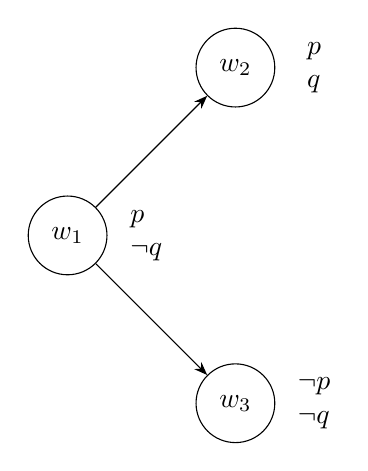
\begin{tikzpicture}[node distance=2cm]

    % 
    \node[draw, circle, minimum size=1cm, inner sep=2pt, align=center] (w1) {$w_1$};
    \node[draw, circle, minimum size=1cm, inner sep=2pt, align=center] (w2) [above right=of w1] {$w_2$};
    \node[draw, circle, minimum size=1cm, inner sep=2pt, align=center] (w3) [below right=of w1] {$w_3$};

    % 
    \node[align=left] at ($(w1) + (1,0)$) {$p$\\$\neg q$};
    \node[align=left] at ($(w2) + (1,0)$) {$p$\\$q$};
    \node[align=left] at ($(w3) + (1,0)$) {$\neg p$\\$\neg q$};

    % 
    \draw[->, >=Stealth] (w1) -- (w2);
    \draw[->, >=Stealth] (w1) -- (w3);

\end{tikzpicture}
}
\end{center}

In this diagram, each circle represents a world, labeled $w_1$, $w_2$, $w_3$, and the propositions that are true in each world are listed next to them. 
The arrows indicate the accessibility relation $R$ between worlds. Formally, when we write $w R w'$, we mean that world $w'$ is accessible from world $w$.

\subsubsection{Truth at a World}

Every modal model specifies which formulas are true at which worlds.

Let
$$M = \langle W, R, V \rangle$$
be a Kripke model over propositional variables $U$. The satisfaction relation
$$M, w \Vdash \varphi$$
means ``$\varphi$ is true at world $w$ in $M$.'' It is defined inductively:

\begin{enumerate}
    \item \textbf{Atomic propositions:}
    $$M, w \Vdash p \leftrightarrow w \in V(p), \quad p \in U$$
    
    \item \textbf{Falsity:}
    $$M, w \nVdash \bot$$
    
    \item \textbf{Negation:}
    $$M, w \Vdash \neg \varphi \leftrightarrow M, w \nVdash \varphi$$
    
    \item \textbf{Conjunction:}
    $$M, w \Vdash \varphi \wedge \psi \leftrightarrow M, w \Vdash \varphi \wedge M, w \Vdash \psi$$
    
    \item \textbf{Disjunction:}
    $$M, w \Vdash \varphi \vee \psi \leftrightarrow M, w \Vdash \varphi \vee M, w \Vdash \psi$$
    
    \item \textbf{Implication:}
    $$M, w \Vdash \varphi \to \psi \leftrightarrow M, w \nVdash \varphi \vee M, w \Vdash \psi$$
    
    \item \textbf{Necessity:}
    $$M, w \Vdash \Box \varphi \leftrightarrow \forall w' \in W, (w,w') \in R \to M, w' \Vdash \varphi$$
    
    \item \textbf{Possibility:}
    $$M, w \Vdash \Diamond \varphi \leftrightarrow \exists w' \in W, (w,w') \in R \wedge M, w' \Vdash \varphi$$
\end{enumerate}

\subsubsection{Truth in a Model}

While
$$M, w \Vdash \varphi$$
represents truth at a specific world $w$ (local truth), we sometimes want global truth: formulas that are true at all worlds in a given model.

$$M \Vdash \varphi \ \Leftrightarrow\ \forall w \in W, \ M, w \Vdash \varphi$$

That is, $\varphi$ holds at every world in $M$.

\begin{enumerate}
    \item If $M \Vdash \varphi$, then $\varphi$ is globally valid in that model.
    \item If $M, w \Vdash \varphi$ for some but not all $w$, then $\varphi$ is only locally true in $M$.
\end{enumerate}

Recall the simple model:

Then we can check which of $p$, $\Box p$, $\Diamond p$, $\Diamond q$ hold and which do not:

\begin{enumerate}
    \item \textbf{For $p$:}
    
    $$M, w_1 \Vdash p \leftrightarrow w_1 \in V(p)$$
    From the model,
    $$w_1 \in V(p)$$
    Therefore,
    $$M, w_1 \Vdash p$$
    
    \item \textbf{For $\Box p$:}
    
    By definition of $\Box$:
    $$M, w_1 \Vdash \Box p \leftrightarrow \forall w' \, (w_1 R w' \to M, w' \Vdash p)$$
    However:
    $$\exists w_3 \, (\, w_1 R w_3 \wedge M, w_3 \nVdash p \,)$$
    Consequently, the universal condition fails.
    Thus,
    $$M, w_1 \nVdash \Box p$$
    
    \item \textbf{For $\Diamond p$:}
    
    By definition of $\Diamond$:
    $$M, w_1 \Vdash \Diamond p \leftrightarrow \exists w' \, (w_1 R w' \wedge M, w' \Vdash p)$$
    From the model,
    $$\exists w_2 (w_1 R w_2 \wedge M, w_2 \Vdash p)$$
    So the existential condition is satisfied.
    It follows that,
    $$M, w_1 \Vdash \Diamond p$$
    
    \item \textbf{For $\Diamond q$:}
    
    Similarly, by definition of $\Diamond$:
    $$M, w_1 \Vdash \Diamond q \leftrightarrow \exists w' \, (w_1 R w' \wedge M, w' \Vdash q)$$
    From the model,
    $$w_1 R w_2 \wedge M, w_2 \Vdash q$$
    Thus, the existential condition is satisfied.
    
    We conclude that:
    $$M, w_1 \Vdash \Diamond q$$
\end{enumerate}

Example 2:

Considering this model:

\begin{figure}[h]
\centering
\fbox{
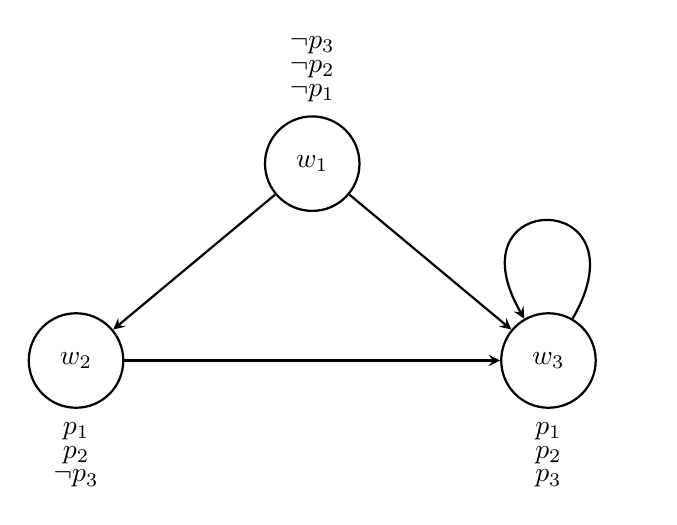
\begin{tikzpicture}[>=stealth, thick]

% 
\node[circle, draw, minimum size=1.2cm] (w1) at (0, 0) {$w_1$};
\node[circle, draw, minimum size=1.2cm] (w2) at (-3, -2.5) {$w_2$};
\node[circle, draw, minimum size=1.2cm] (w3) at (3, -2.5) {$w_3$};

% 
\node at (0, 0.9) {$\neg p_1$};
\node at (0, 1.2) {$\neg p_2$};
\node at (0, 1.5) {$\neg p_3$};

% 
\node at (-3, -3.4) {$p_1$};
\node at (-3, -3.7) {$p_2$};
\node at (-3, -4.0) {$\neg p_3$};

% 
\node at (3, -3.4) {$p_1$};
\node at (3, -3.7) {$p_2$};
\node at (3, -4.0) {$p_3$};

% 
\draw[->] (w1) -- (w2);
\draw[->] (w1) -- (w3);
\draw[->] (w2) -- (w3);
\draw[->] (w3) to[out=60, in=120, looseness=8] (w3);

\end{tikzpicture}
}
\end{figure}

From the Kripke model $M = (W,R,V)$ depicted above, we now evaluate the formulas.

Accessibility relation:
$$R = \{ (w_1, w_2), (w_1, w_3), (w_2, w_3), (w_3, w_3) \}$$

\begin{enumerate}
    \item $p \to \Diamond p$ (atomic $p$)
    
    $$M, w \Vdash p \to \Diamond p \leftrightarrow M, w \nVdash p \vee M, w \Vdash \Diamond p$$
    
    $$M, w \Vdash \Diamond p \leftrightarrow \exists w' \in W: w R w' \wedge M, w' \Vdash p$$
    
    $$\therefore \forall w \in W: M, w \Vdash p \to \Diamond p$$
    
    \item $A \to \Diamond A$ (arbitrary $A$)
    
    $$M, w \Vdash A \to \Diamond A \leftrightarrow M, w \nVdash A \vee M, w \Vdash \Diamond A$$
    
    $$M, w \Vdash \Diamond A \leftrightarrow \exists w' \in W: w R w' \wedge M, w' \Vdash A$$
    
    $$\therefore \forall w \in W: M, w \Vdash A \to \Diamond A$$
    
    \item $\Box p \to p$ (atomic $p$)
    
    $$M, w \Vdash \Box p \to p \leftrightarrow M, w \nVdash \Box p \vee M, w \Vdash p$$
    
    $$M, w \Vdash \Box p \leftrightarrow \forall w' \in W: w R w' \to M, w' \Vdash p$$
    
    $$\therefore \forall w \in W: M, w \Vdash \Box p \to p$$
    
    \item $\neg p \to \Diamond \Box p$ (atomic $p$)
    
    $$M, w \Vdash \neg p \to \Diamond \Box p \leftrightarrow M, w \nVdash \neg p \vee M, w \Vdash \Diamond \Box p$$
    
    $$M, w \Vdash \Diamond \Box p \leftrightarrow \exists w' \in W: w R w' \wedge M, w' \Vdash \Box p$$
    
    $$\therefore \forall w \in W: M, w \Vdash \neg p \to \Diamond \Box p$$
    
    \item $\Diamond \Box A$ (arbitrary $A$)
    
    Let $A = p_1 \wedge \neg p_3$
    
    $$M, w \Vdash \Diamond \Box A \leftrightarrow \exists w' \in W: w R w' \wedge M, w' \Vdash \Box A$$
    
    $$M, w_2 \Vdash A \wedge \forall w': w_2 R w', M, w' \nVdash A \to M, w_2 \nVdash \Diamond \Box A$$
    
    $$\therefore \exists w \in W: M, w \nVdash \Diamond \Box A$$
    
    \item $\Box \Diamond p$ (atomic $p$)
    
    $$M, w \Vdash \Box \Diamond p \leftrightarrow \forall w' \in W: w R w' \to M, w' \Vdash \Diamond p$$
    
    $$M, w' \Vdash \Diamond p \leftrightarrow \exists w'': w' R w'' \wedge M, w'' \Vdash p$$
    
    $$\therefore \forall w \in W: M, w \Vdash \Box \Diamond p$$
\end{enumerate}

\subsection{Validity}

Validity in modal logic is always a property of formulas. A formula is called valid if it holds in every model and at every world of that model. However, which formulas count as valid depends on the semantics, in particular, on the accessibility relation $R$ that structures the models.

For example:

$$\models \Box(p \land q) \to \Box p$$

is valid in all Kripke models, since if every accessible world satisfies both $p$ and $q$, then certainly every accessible world satisfies $p$.

\textit{Proof:}

Let
$$M = (W, R, V)$$
be an arbitrary Kripke model and let
$$w \in W$$
be an arbitrary world. We need to show:

$$M, w \Vdash \Box(p \land q) \to \Box p$$

First, assume the antecedent

$$M, w \Vdash \Box(p \land q)$$

By the semantics of $\Box$, this means:

$$\forall w' \in W, \text{ if } w R w' \text{ then } M, w' \Vdash p \land q$$

Second, for each world $w'$ such that $w R w'$:

$$M, w' \Vdash p \land q \to M, w' \Vdash p$$

Moreover, generalize over accessible worlds.

Since the above holds for all $w'$ accessible from $w$, we have:

$$\forall w' \in W, \text{ if } w R w' \text{ then } M, w' \Vdash p$$

By the semantics of $\Box$, this is equivalent to:

$$M, w \Vdash \Box p$$

Finally, we conclude the implication

$$M, w \Vdash \Box(p \land q) \to M, w \Vdash \Box p$$

Ultimately,

$$M, w \Vdash \Box(p \land q) \to \Box p$$

Since $M$ and $w$ were arbitrary, the formula holds in every world of every Kripke model.

Therefore,

$$\models \Box(p \land q) \to \Box p. \quad \text{QED}$$

\begin{figure}[h]
\centering
\fbox{
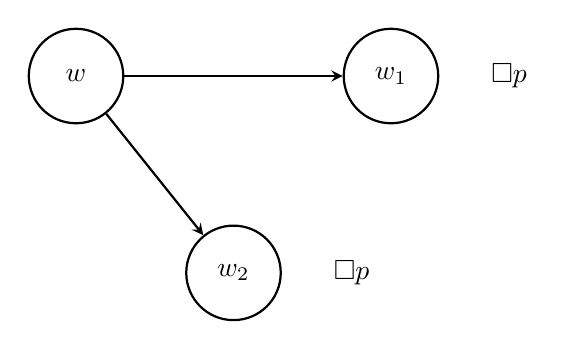
\begin{tikzpicture}[>=stealth, thick]

% 
\node[circle, draw, minimum size=1.2cm] (w) at (0, 0) {$w$};
\node[circle, draw, minimum size=1.2cm] (w1) at (4, 0) {$w_1$};
\node[circle, draw, minimum size=1.2cm] (w2) at (2, -2.5) {$w_2$};

% 
\node at (5.5, 0) {$\Box p$};
\node at (3.5, -2.5) {$\Box p$};

% 
\draw[->] (w) -- (w1);
\draw[->] (w) -- (w2);

\end{tikzpicture}
}
\end{figure}

Another example:

$$\Box(p \to q) \not\models p \to \Box q$$

and

$$p \to \Box q \not\models \Box(p \to q)$$

\textit{Proof (by counterexample):}

Let
$$M = (W,R,V), \quad W = \{w,v\}, \quad R = \{(w,v)\},$$
with valuation
$$V(p) = \{w\}, \quad V(q) = \varnothing.$$

At world $w$:

\begin{enumerate}
    \item Antecedent:
    $$M,w \Vdash \Box(p \to q)$$
    because the only accessible world is $v$, and there $p$ is false, so $p \to q$ is true.
    
    \item Consequent:
    $$M,w \not\Vdash p \to \Box q$$
    since $M,w \Vdash p$ but $M,w \not\Vdash \Box q$ (because $q$ is false at $v$).
    
    Therefore,
    $$\Box(p \to q) \not\models p \to \Box q.$$
\end{enumerate}

\begin{center}
\fbox{
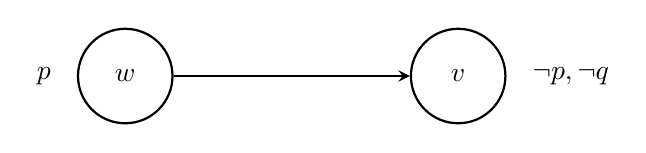
\begin{tikzpicture}[node distance=3cm,->,>=stealth,thick]

   
  \tikzstyle{world}=[circle,draw,minimum size=1.2cm,align=center]

   
  \node[world] (w) {$w$};
  \node[world] (v) [right=of w] {$v$};

   
  \draw (w) -- (v);

   
  \node[left=0.2cm of w] {$p$};
  \node[right=0.2cm of v] {$\neg p, \neg q$};

\end{tikzpicture}
}
\end{center}

This model makes $\Box(p \to q)$ true at $w$ but $p \to \Box q$ false.

Let
$$M = (W,R,V), \quad W = \{w,v\}, \quad R = \{(w,v)\},$$
with valuation
$$V(p) = \{v\}, \quad V(q) = \varnothing.$$

At world $w$:

\begin{enumerate}
    \item Antecedent:
    
    $$M,w \Vdash p \to \Box q$$
    because $M,w \not\Vdash p$, so the implication holds.
    
    \item Consequent:
    
    $$M,w \not\Vdash \Box(p \to q)$$
    since at $v$, $M,v \Vdash p$ but $M,v \not\Vdash q$, so $p \to q$ is false at $v$.
    
    Therefore,
    $$p \to \Box q \not\models \Box(p \to q). \quad \text{QED}$$
\end{enumerate}

\begin{center}
\fbox{
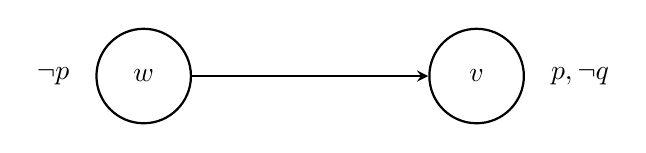
\begin{tikzpicture}[node distance=3cm,->,>=stealth,thick]

   
  \tikzstyle{world}=[circle,draw,minimum size=1.2cm,align=center]

   
  \node[world] (w) {$w$};
  \node[world] (v) [right=of w] {$v$};

   
  \draw (w) -- (v);

   
  \node[left=0.2cm of w] {$\neg p$};
  \node[right=0.2cm of v] {$p, \neg q$};

\end{tikzpicture}
}
\end{center}

This model makes $p \to \Box q$ true at $w$ but $\Box(p \to q)$ false.

Moreover:

\begin{enumerate}
    \item If $A$ is valid in $U$, then $A$ is valid in every subclass $U' \subseteq U$.
    \item If $A$ is valid, then $\Box A$ is also valid.
\end{enumerate}

Example:

$$\models \Box X$$

\textit{Proof.}

Assume
$$\models X$$
i.e. $X$ is valid in every Kripke model.

Let
$$M = \langle W, R, V \rangle$$
be an arbitrary Kripke model and let $w \in W$.

Since $X$ is valid, for every world $w' \in W$ we have
$$M, w' \Vdash X$$

Now suppose $w R w'$. By validity of $X$, it follows again that
$$M, w' \Vdash X$$

Therefore, by the semantics of $\Box$, we obtain
$$M, w \Vdash \Box X$$

Since both $M$ and $w$ were arbitrary, we conclude
$$\models \Box X$$

\subsection{Tautology}

In classical logic, it is easy to check whether a formula is a tautology or not. For example,

$$P \lor \neg P$$

is a tautology, and we can also prove this using a truth table. However, in modal logic the term \textit{tautology} is usually not used. Instead, we talk about \textit{valid formulas}, since the semantics of modal logic are more complex than in classical logic. In this context, the concept of simultaneous substitution becomes helpful.

For example, recall

$$\varphi \equiv (\psi \leftrightarrow \chi)$$

Then under simultaneous substitution we have

$$\varphi[\delta_1/p_1, \ldots, \delta_n/p_n] \;=\; 
\psi[\delta_1/p_1, \ldots, \delta_n/p_n] \;\leftrightarrow\; 
\chi[\delta_1/p_1, \ldots, \delta_n/p_n].$$

In other words, substitution distributes structurally through the connectives.

\section{Modal Equivalence}

\subsection{Basic Duality}
\begin{enumerate}
\item $\Diamond X \equiv \neg \Box \neg X \quad \text{(Definition of possibility)}$
\item $\Box X \equiv \neg \Diamond \neg X \quad \text{(Definition of necessity)}$
\item $\neg \Diamond X \equiv \Box \neg X \quad \text{(Negation of possibility)}$
\item $\neg \Box X \equiv \Diamond \neg X \quad \text{(Negation of necessity)}$
\end{enumerate}

\subsection{Double Negation}
\begin{enumerate}
\setcounter{enumi}{4}
\item $\Box \neg \neg X \equiv \Box X \quad \text{(Double negation in necessity)}$
\item $\Diamond \neg \neg X \equiv \Diamond X \quad \text{(Double negation in possibility)}$
\item $\neg \neg \Box X \equiv \Box X \quad \text{(Double negation outside)}$
\item $\neg \neg \Diamond X \equiv \Diamond X \quad \text{(Double negation outside)}$
\end{enumerate}

\subsection{De Morgan's Laws for Modalities}
\begin{enumerate}
\setcounter{enumi}{8}
\item $\neg(\Box X \land \Box Y) \equiv \Diamond \neg X \lor \Diamond \neg Y \quad \text{(De Morgan's)}$
\item $\neg(\Diamond X \lor \Diamond Y) \equiv \Box \neg X \land \Box \neg Y \quad \text{(De Morgan's)}$
\item $\neg(\Box X \lor \Box Y) \equiv \Diamond \neg X \land \Diamond \neg Y \quad \text{(De Morgan's)}$
\item $\neg(\Diamond X \land \Diamond Y) \equiv \Box \neg X \lor \Box \neg Y \quad \text{(De Morgan's)}$
\end{enumerate}

\subsection{Implication Equivalences}
\begin{enumerate}
\setcounter{enumi}{12}
\item $X \to Y \equiv \neg X \lor Y \quad \text{(Material implication)}$
\item $\neg(X \to Y) \equiv X \land \neg Y \quad \text{(Negation of implication)}$
\item $X \to Y \equiv \neg Y \to \neg X \quad \text{(Contrapositive)}$
\item $\Box X \to \Box Y \equiv \neg \Box Y \to \neg \Box X \quad \text{(Modal contrapositive)}$
\item $\Diamond X \to \Diamond Y \equiv \neg \Diamond Y \to \neg \Diamond X \quad \text{(Modal contrapositive)}$
\end{enumerate}

\subsection{Conjunction and Disjunction}
\begin{enumerate}
\setcounter{enumi}{17}
\item $\Box(X \land Y) \equiv \Box X \land \Box Y \quad \text{(Distribution over conjunction)}$
\item $\Diamond(X \lor Y) \equiv \Diamond X \lor \Diamond Y \quad \text{(Distribution over disjunction)}$
\end{enumerate}
\subsection{Substitution Lemma}

To justify this notion (e.g. $\varphi \equiv (\psi \leftrightarrow \chi)$), we prove the Substitution Lemma, which shows that the truth of propositional formulas under an assignment aligns with the truth of their tautological instances in Kripke models.

Suppose $X$ is a modal-free formula whose propositional variables are $x_1, \ldots, x_n$, and let $\delta_1, \ldots, \delta_n$ be modal formulas. Then for any assignment $v$, any model $M = \langle W, R, V \rangle$, and any $w \in W$ such that

$$v(x_i) = T \quad \text{iff} \quad M,w \Vdash \delta_i,$$

we have

$$v \Vdash X \quad \text{iff} \quad M,w \Vdash X[\delta_1/x_1, \ldots, \delta_n/x_n].$$

\textit{Proof.} By induction on the structure of $X$.

\begin{enumerate}
    \item \textbf{Atomic variable:}
    
    $$X \equiv x_i$$
    $$v \Vdash x_i \leftrightarrow v(x_i) = T 
    \leftrightarrow M,w \Vdash \delta_i
    \leftrightarrow M,w \Vdash x_i[\delta_1/x_1, \ldots, \delta_n/x_n].$$
    
    \item \textbf{Falsity:}
    
    $$X \equiv \bot$$
    $$v \nVdash \bot \quad \text{and} \quad M,w \nVdash \bot$$
    
    \item \textbf{Negation:}
    
    $$X \equiv \neg \alpha$$
    $$v \Vdash \neg \alpha \leftrightarrow v \nVdash \alpha
    \leftrightarrow M,w \nVdash \alpha[\delta_1/x_1, \ldots, \delta_n/x_n]
    \leftrightarrow M,w \Vdash \neg \alpha[\delta_1/x_1, \ldots, \delta_n/x_n].$$
    
    \item \textbf{Conjunction:}
    
    $$X \equiv (\alpha \land \beta)$$
    $$v \Vdash \alpha \land \beta \leftrightarrow (v \Vdash \alpha \land v \Vdash \beta)$$
    $$\leftrightarrow (M,w \Vdash \alpha[\delta_1/x_1, \ldots, \delta_n/x_n] \land M,w \Vdash \beta[\delta_1/x_1, \ldots, \delta_n/x_n])$$
    $$\leftrightarrow M,w \Vdash (\alpha \land \beta)[\delta_1/x_1, \ldots, \delta_n/x_n].$$
    
    \item \textbf{Disjunction:}
    
    $$X \equiv (\alpha \lor \beta)$$
    $$v \Vdash \alpha \lor \beta \leftrightarrow (v \Vdash \alpha \lor v \Vdash \beta)$$
    $$\leftrightarrow (M,w \Vdash \alpha[\delta_1/x_1, \ldots, \delta_n/x_n] \lor M,w \Vdash \beta[\delta_1/x_1, \ldots, \delta_n/x_n])$$
    $$\leftrightarrow M,w \Vdash (\alpha \lor \beta)[\delta_1/x_1, \ldots, \delta_n/x_n].$$
    
    \item \textbf{Implication:}
    
    $$X \equiv (\alpha \to \beta)$$
    $$v \Vdash \alpha \to \beta \leftrightarrow (v \nVdash \alpha \lor v \Vdash \beta)$$
    $$\leftrightarrow (M,w \nVdash \alpha[\delta_1/x_1, \ldots, \delta_n/x_n] \lor M,w \Vdash \beta[\delta_1/x_1, \ldots, \delta_n/x_n])$$
    $$\leftrightarrow M,w \Vdash (\alpha \to \beta)[\delta_1/x_1, \ldots, \delta_n/x_n].$$
\end{enumerate}

From this lemma we can show that all tautological instances are valid.

\textit{Proof.}

Contrapositively, suppose $U$ is such that

$$M,w \nVdash U[\delta_1/x_1,\ldots, \delta_n/x_n]$$

for some model $M$ and world $w$. Define an assignment $v$ such that

$$v(x_i) = T \quad \leftrightarrow \quad M,w \Vdash \delta_i,$$

and let $v$ assign arbitrary values to $q \notin \{x_1, \ldots, x_n\}$. Then by the lemma,

$$v \Vdash U,$$

so $U$ is not a tautology.

\section{Schema}

One could say that a schema is a set of formulas comprising all and only the substitution instances of some modal formula. For example, the schema $\Box(A \to B) \to (\Box A \to \Box B)$ includes all formulas of the form $\Box(x \to y) \to (\Box x \to \Box y)$ where $x$ and $y$ are any well-formed formulas in our modal language.

\subsection{Formal Definition}

A schema is a collection of formulas consisting precisely of all substitution instances of a given modal formula $\varphi$. Formally:

$$\{ \psi : \exists \delta_1, \ldots, \delta_n\; (\psi = \varphi[\delta_1/x_1, \ldots,\delta_n/x_n]) \}$$

The formula $\varphi$ is called the characteristic formula of the schema, and it is unique up to renaming of propositional variables. A formula $\psi$ is said to be an instance of a schema if $\psi$ belongs to this set.

For convenience, a schema is usually denoted by a meta-linguistic expression obtained by substituting symbols such as $A, B, \dots$ for propositional variables. For example:

\begin{enumerate}
    \item The schema $A$ corresponds to the characteristic formula $p$.
    \item The schema $A \to \Box A$ corresponds to $p \to \Box p$.
    \item The schema $A \to (B \to A)$ corresponds to $p \to (q \to p)$.
\end{enumerate}

In particular, the schema $A$ denotes the set of all formulas, since every formula is a substitution instance of $p$.

\subsection{Truth and Validity}

A schema is said to be true in a model if and only if all of its instances are true in that model. Similarly, a schema is valid if and only if it is true in every model. Valid schemas have a particularly important connection with the axiom schema $K$:

$$K = \Box(A \to B) \to (\Box A \to \Box B).$$

It can be shown that $K$ is valid in every model. Because of this, schema $K$ serves as the cornerstone of the modal system $K$, the weakest normal modal logic.

\subsection{Valid Schemas}

The following schemas are valid in every Kripke model:

\begin{enumerate}
    \item $\Box(A \to B) \to (\Diamond A \to \Diamond B)$
    \item $\Diamond(A \to B) \to (\Box A \to \Diamond B)$
    \item $\Box(A \land B) \leftrightarrow (\Box A \land \Box B)$
    \item $\Box A \to \Box(B \to A)$
    \item $\neg \Diamond A \to \Box(A \to B)$
    \item $\Diamond(A \lor B) \leftrightarrow (\Diamond A \lor \Diamond B)$
    \item $\Diamond A \leftrightarrow \neg \Box \neg A$ 
\end{enumerate}

\newpage
\textbf{Example:}

Let $M = (W, R, V)$ be an arbitrary Kripke model and $w \in W$ an arbitrary world. We show the duality of $\Diamond$ and $\Box$:

\begin{enumerate}
    \item By definition:
    $$M, w \Vdash \neg \Box \neg A \leftrightarrow M, w \nVdash \Box \neg A$$
    
    \item By the semantics of $\Box$:
    $$M, w \Vdash \Box \neg A \leftrightarrow \forall w' \in W,\, (w R w' \implies M, w' \Vdash \neg A)$$
    Therefore:
    $$M, w \nVdash \Box \neg A \leftrightarrow \neg (\forall w' \in W,\, w R w' \implies M, w' \Vdash \neg A)$$
    
    \item Negating the universal gives an existential:
    $$\neg (\forall w' \in W,\, w R w' \implies M, w' \Vdash \neg A) \leftrightarrow \exists w' \in W,\, (w R w' \wedge M, w' \nVdash \neg A)$$
    
    \item By classical negation:
    $$M, w' \nVdash \neg A \leftrightarrow M, w' \Vdash A$$
    
    \item By definition of $\Diamond$:
    $$\exists w' \in W,\, (w R w' \wedge M, w' \Vdash A) \leftrightarrow M, w \Vdash \Diamond A$$
\end{enumerate}

Thus, for an arbitrary model $M$ and world $w$:
$$M, w \Vdash \Diamond A \leftrightarrow M, w \Vdash \neg \Box \neg A$$

Since $M$ and $w$ were arbitrary, the formula is valid in all Kripke models:
$$\models \Diamond A \leftrightarrow \neg \Box \neg A$$

\subsection{Invalid Schemas}

To show that a formula $\varphi$ is invalid, we construct a model $M$ and a world $w$ such that

$$M, w \not\Vdash \varphi.$$

Such models are called falsifying models. To show that a schema $X$ is invalid, it suffices to construct a falsifying model for one of its instances.

\textbf{Example 1:}

Schema $D$ is
$$\Box p \to \Diamond p.$$

Counterexample:

Let
$$M=(W,R,V)$$
with
$$W=\{w\},\quad R=\varnothing,\quad V(p)=\varnothing.$$

\begin{enumerate}
    \item Antecedent:
    $$M,w \Vdash \Box p
    \leftrightarrow \forall v\in W\,(wRv\to M,v \Vdash p).$$
    Since $R=\varnothing$,
    $$M,w \Vdash \Box p.$$
    
    \item Consequent:
    $$M,w \Vdash \Diamond p
    \leftrightarrow \exists v\in W\,(wRv\land M,v \Vdash p).$$
    Since $R=\varnothing$,
    $$M,w\not \Vdash \Diamond p.$$
    
    \item Therefore:
    $$M,w\not \Vdash \Box p \to \Diamond p.$$
    
    Hence $\Box p \to \Diamond p$ is not valid. $\quad \text{Q.E.D.}$
\end{enumerate}

\begin{center}
\fbox{
\begin{tikzpicture}[node distance=2.5cm,->,>=stealth,thick]
  \tikzstyle{world}=[circle,draw,minimum size=1.2cm,align=center]

   
  \node[world,label=below:$\neg p$] (w) at (0,0) {$w$};

   
  \node[world] (w1) at (-4,0) {$w_1$};
  \node[world] (w2) at (4,0) {$w_2$};
  \node[world] (w3) at (0,4) {$w_3$};
  \node[world] (w4) at (0,-4) {$w_4$};

   

   
  \node[below=0.6cm of w] {$M, w \not\Vdash \Box p \to \Diamond p$};
\end{tikzpicture}
}
\end{center}

\textbf{Example 2:}

Schema $T$ is
$$\Box p \to p.$$

Counterexample:

Let
$$M=(W,R,V)$$
with
$$W=\{w\},\quad R=\varnothing,\quad V(p)=\varnothing.$$

\begin{enumerate}
    \item Antecedent:
    $$M,w\Vdash\Box p
    \leftrightarrow \forall v\in W\,(wRv \to M,v\Vdash p).$$
    Since $R=\varnothing$,
    $$M,w\Vdash\Box p.$$
    
    \item Consequent:
    $$M,w\Vdash p$$
    is false because $V(p)=\varnothing$. Hence
    $$M,w\not\Vdash p.$$
    
    \item Therefore:
    $$M,w\not\Vdash \Box p \to p.$$
    
    Hence $\Box p \to p$ is not valid. $\quad \text{Q.E.D.}$
\end{enumerate}

\begin{center}
\fbox{
\begin{tikzpicture}[node distance=2.5cm,->,>=stealth,thick]
  \tikzstyle{world}=[circle,draw,minimum size=1.2cm,align=center]

   
  \node[world,label=below:$\neg p$] (w) at (0,0) {$w$};

   
  \node[world] (w1) at (-4,0) {$w_1$};
  \node[world] (w2) at (4,0) {$w_2$};
  \node[world] (w3) at (0,4) {$w_3$};
  \node[world] (w4) at (0,-4) {$w_4$};

  

   
  \node[below=0.6cm of w] {$M, w \not\Vdash \Box p \to p$};
\end{tikzpicture}
}
\end{center}

\textbf{Example 3:}

Schema $B$ is:
$$p \to \Box\Diamond p.$$

Counterexample:

Let
$$M=(W,R,V)$$
with
$$W=\{w,v\},\quad R=\{(w,v)\},\quad V(p)=\{w\}.$$

\begin{enumerate}
    \item Antecedent:
    $$M,w\Vdash p$$
    since $w\in V(p)$.
    
    \item Consequent:
    $$M,w\Vdash\Box\Diamond p
    \leftrightarrow \forall x\in W\,(wRx\to M,x\Vdash\Diamond p).$$
    There is $x=v$ with $wRv$. But
    $$M,v\Vdash\Diamond p
    \leftrightarrow \exists u\in W\,(vRu\land M,u\Vdash p),$$
    and there is no $u$ with $vRu$. Hence
    $$M,v\not\Vdash\Diamond p,$$
    so
    $$M,w\not\Vdash\Box\Diamond p.$$
    
    \item Therefore:
    $$M,w\not\Vdash p\to\Box\Diamond p.$$
    
    Hence $p\to\Box\Diamond p$ is not valid. $\quad \text{Q.E.D.}$
\end{enumerate}

\begin{center}
\fbox{
\begin{tikzpicture}[->,>=stealth,thick,node distance=2.5cm]
  \tikzstyle{world}=[circle,draw,minimum size=1.2cm,align=center]

   
  \node[world,label=below:$p$] (w) at (0,0) {$w$};
  \node[world,label=below:$\neg p$] (v) at (4,0) {$v$};

   
  \node[world] (w1) at (-4,0) {$w_1$};
  \node[world] (w2) at (0,4) {$w_2$};
  \node[world] (w3) at (0,-4) {$w_3$};

   
  \draw (w) -- (v);

   
  \node[below=0.6cm of w] {$M, w \not\Vdash p \to \Box\Diamond p$};
\end{tikzpicture}
}
\end{center}

\textbf{Example 4:}

Schema $4$ is
$$\Box p \to \Box\Box p.$$

Counterexample:

Let
$$M=(W,R,V)$$
with
$$W=\{w,v,u\},\quad R=\{(w,v),(v,u)\},\quad V(p)=\{v\}.$$

\begin{enumerate}
    \item Antecedent:
    $$M,w\Vdash\Box p
    \leftrightarrow \forall x\in W\,(wRx\to M,x\Vdash p).$$
    The only $x$ with $wRx$ is $v$, and $v\in V(p)$, so
    $$M,w\Vdash\Box p.$$
    
    \item Consequent:
    $$M,w\Vdash\Box\Box p
    \leftrightarrow \forall x\in W\,(wRx\to M,x\Vdash\Box p).$$
    For $x=v$ we have
    $$M,v\Vdash\Box p
    \leftrightarrow \forall y\in W\,(vRy\to M,y\Vdash p).$$
    But $vRu$ and $u\notin V(p)$, hence
    $$M,v\not\Vdash\Box p,$$
    so
    $$M,w\not\Vdash\Box\Box p.$$
    
    \item Therefore:
    $$M,w\not\Vdash \Box p \to \Box\Box p.$$
    
    Hence $\Box p \to \Box\Box p$ is not valid. $\quad \text{Q.E.D.}$
\end{enumerate}

\begin{center}
\fbox{
\begin{tikzpicture}[->,>=stealth,thick,node distance=2.5cm]
  \tikzstyle{world}=[circle,draw,minimum size=1.2cm,align=center]

   
  \node[world,label=below:$\neg p$] (w) at (0,0) {$w$};
  \node[world,label=below:$p$] (v) at (4,0) {$v$};
  \node[world,label=below:$\neg p$] (u) at (8,0) {$u$};

  
  \node[world] (w1) at (0,4) {$w_1$};
  \node[world] (w2) at (0,-4) {$w_2$};

  
  \draw (w) -- (v);
  \draw (v) -- (u);

  
  \node[below=0.6cm of w, xshift=4cm] {$M, w \not\Vdash \Box p \to \Box\Box p$};
\end{tikzpicture}
}
\end{center}

\textbf{Example 5:}

Schema $5$:
$$\Diamond p \to \Box\Diamond p.$$

Counterexample:

Let
$$M=(W,R,V)$$
with
$$W=\{w,v\},\quad R=\{(w,v)\},\quad V(p)=\{v\}.$$

\begin{enumerate}
    \item Antecedent:
    $$M,w\Vdash\Diamond p
    \leftrightarrow \exists x\in W\,(wRx\land M,x\Vdash p).$$
    Since $wRv$ and $v\in V(p)$,
    $$M,w\Vdash\Diamond p.$$
    
    \item Consequent:
    $$M,w\Vdash\Box\Diamond p
    \leftrightarrow \forall x\in W\,(wRx\to M,x\Vdash\Diamond p).$$
    The only $x$ with $wRx$ is $v$, and
    $$M,v\Vdash\Diamond p
    \leftrightarrow \exists y\in W\,(vRy\land M,y\Vdash p).$$
    There is no $y$ with $vRy$, hence
    $$M,v\not\Vdash\Diamond p,$$
    so
    $$M,w\not\Vdash\Box\Diamond p.$$
    
    \item Therefore:
    $$M,w\not\Vdash \Diamond p \to \Box\Diamond p.$$
\end{enumerate}

Hence $\Diamond p \to \Box\Diamond p$ is not valid. $\quad \text{Q.E.D.}$

\begin{center}
\fbox{
\begin{tikzpicture}[->,>=stealth,thick,node distance=2.5cm]
  \tikzstyle{world}=[circle,draw,minimum size=1.2cm,align=center]

   
  \node[world,label=below:$\neg p$] (w) at (0,0) {$w$};
  \node[world,label=below:$p$] (v) at (4,0) {$v$};

   
  \node[world] (w1) at (-4,0) {$w_1$};
  \node[world] (w2) at (0,4) {$w_2$};
  \node[world] (w3) at (0,-4) {$w_3$};

  
  \draw (w) -- (v);

   
  \node[below=0.6cm of w] {$M, w \not\Vdash \Diamond p \to \Box\Diamond p$};
\end{tikzpicture}
}
\end{center}

\subsubsection{Combining Frame Properties}

\begin{enumerate}
    \item \textbf{$T+4 = (S4)$}
    
    Suppose
    $$M = (W, R, V), \quad W = \{w, v, u\}$$
    with the relation
    $$R = \{(w,w), (v,v), (u,u), (w,v), (v,u), (w,u)\}.$$
    
    Reflexivity ($T$):
    $$\forall x \in W \; (xRx)$$
    Holds, since $wRw, vRv, uRu \in R$.
    
    Transitivity ($4$):
    $$\forall x,y,z \in W \; (xRy \wedge yRz \;\to\; xRz)$$
    Holds, since $wRv \wedge vRu \;\to\; wRu \in R$.
    
    Modal validity at $w$:
    $$M,w \Vdash \Box p \to p$$
    $$M,w \Vdash \Box p \to \Box \Box p$$
    
    Thus, $R$ is reflexive and transitive, validating $S4$.
    
    \item \textbf{$T+B$}
    
    Suppose
    $$M = (W, R, V), \quad W = \{w, v, u\}$$
    with the relation
    $$R = \{(w,w), (v,v), (u,u), (w,v), (v,w)\}.$$
    
    Reflexivity ($T$):
    $$\forall x \in W \; (xRx)$$
    Holds.
    
    Symmetry ($B$):
    $$\forall x,y \in W \; (xRy \;\to\; yRx)$$
    Holds.
    
    Modal validity at $w$:
    $$M,w \Vdash \Box p \to p$$
    $$M,w \Vdash p \to \Box \Diamond p$$
    
    Thus, $R$ is reflexive and symmetric.
    
    \item \textbf{$T+5 =(S5)$}
    
    Suppose
    $$M = (W, R, V), \quad W = \{w, v, u\}$$
    with the relation
    $$R = W \times W.$$
    
    Reflexivity ($T$):
    $$\forall x \in W \; (xRx)$$
    Holds.
    
    Euclidean ($5$):
    $$\forall x,y,z \in W \; (xRy \wedge xRz \;\to\; yRz)$$
    Holds.
    
    Modal validity at $w$:
    $$M,w \Vdash \Box p \to p$$
    $$M,w \Vdash \Diamond p \to \Box \Diamond p$$
    
    Thus, $R$ is reflexive and euclidean, validating $S5$.
    
    \item \textbf{$B+5$}
    
    Suppose
    $$M = (W, R, V), \quad W = \{w, v, u\}$$
    with the relation
    $$R = \{(w,w), (v,v), (u,u), (w,v), (v,w), (v,u), (u,v)\}.$$
    
    Symmetry ($B$):
    $$\forall x,y \in W \; (xRy \;\to\; yRx)$$
    Holds.
    
    Euclidean ($5$):
    $$\forall x,y,z \in W \; (xRy \wedge xRz \;\to\; yRz)$$
    Holds.
    
    Modal validity at $w$:
    $$M,w \Vdash p \to \Box \Diamond p$$
    $$M,w \Vdash \Diamond p \to \Box \Diamond p$$
    
    Thus, $R$ is symmetric and euclidean.
    
    \item \textbf{$4+5$}
    
    Suppose
    $$M = (W, R, V), \quad W = \{w, v, u\}$$
    with the relation
    $$R = \{(w,w), (v,v), (u,u), (w,v), (v,u), (w,u)\}.$$
    
    Transitivity ($4$):
    $$\forall x,y,z \in W \; (xRy \wedge yRz \;\to\; xRz)$$
    Holds.
    
    Euclidean ($5$):
    $$\forall x,y,z \in W \; (xRy \wedge xRz \;\to\; yRz)$$
    Holds.
    
    Modal validity at $w$:
    $$M,w \Vdash \Box p \to \Box \Box p$$
    $$M,w \Vdash \Diamond p \to \Box \Diamond p$$
    
    Thus, $R$ is both transitive and euclidean.
\end{enumerate}

\subsubsection{Logical Relationships Between Properties}

\begin{enumerate}
    \item \textbf{$T \to D$}
    
    \textit{Proof:}
    
    Assume R is reflexive:
    $$\forall w \in W: wRw$$
    
    We need to show R is serial:
    $$\forall w \in W: \exists v \in W: wRv$$
    
    Let $w \in W$ be arbitrary.
    
    By reflexivity:
    $$wRw$$
    
    Therefore:
    $$\exists v \in W: wRv \quad (v = w)$$
    
    Since $w$ was arbitrary:
    $$\forall w \in W: \exists v \in W: wRv$$
    
    Therefore, R is serial. $\quad \text{QED}$
    
    \item \textbf{$B + 4 \to 5$}
    
    \textit{Proof:}
    
    Assume R is symmetric:
    $$\forall x, y \in W: xRy \to yRx$$
    
    Assume R is transitive:
    $$\forall x, y, z \in W: (xRy \land yRz) \to xRz$$
    
    We need to show R is Euclidean:
    $$\forall x, y, z \in W: (xRy \land xRz) \to yRz$$
    
    Let $x, y, z \in W$ be arbitrary. Assume:
    $$xRy \land xRz$$
    
    From the assumption:
    $$xRy \quad \text{and} \quad xRz$$
    
    By symmetry applied to $xRy$:
    $$xRy \to yRx$$
    
    Therefore:
    $$yRx$$
    
    Now we have:
    $$yRx \land xRz$$
    
    By transitivity:
    $$(yRx \land xRz) \to yRz$$
    
    Therefore:
    $$yRz$$
    
    This completes the implication:
    $$(xRy \land xRz) \to yRz$$
    
    Since $x, y, z$ were arbitrary:
    $$\forall x, y, z \in W: (xRy \land xRz) \to yRz$$
    
    It follows that R is Euclidean. $\quad \text{QED}$
    
    \item \textbf{$T + 5 \to B$}
    
    \textit{Proof:}
    
    Assume R is reflexive:
    $$\forall w \in W: wRw$$
    
    Assume R is Euclidean:
    $$\forall x, y, z \in W: (xRy \land xRz) \to yRz$$
    
    We need to show R is symmetric:
    $$\forall x, y \in W: xRy \to yRx$$
    
    Let $x, y \in W$ be arbitrary. Assume:
    $$xRy$$
    
    By reflexivity:
    $$xRx$$
    
    Now we have:
    $$xRy \land xRx$$
    
    By the Euclidean property applied to $x, y, x$:
    $$(xRy \land xRx) \to yRx$$
    
    Therefore:
    $$yRx$$
    
    This completes the implication:
    $$xRy \to yRx$$
    
    Since $x, y$ were arbitrary:
    $$\forall x, y \in W: xRy \to yRx$$
    
    We conclude that R is symmetric. $\quad \text{QED}$
    
    \item \textbf{$B + 5 \to 4$}
    
    \textit{Proof:}
    
    Assume R is symmetric:
    $$\forall x, y \in W: xRy \to yRx$$
    
    Assume R is Euclidean:
    $$\forall x, y, z \in W: (xRy \land xRz) \to yRz$$
    
    We need to show R is transitive:
    $$\forall x, y, z \in W: (xRy \land yRz) \to xRz$$
    
    Let $x, y, z \in W$ be arbitrary. Assume:
    $$xRy \land yRz$$
    
    From the assumption:
    $$xRy \quad \text{and} \quad yRz$$
    
    By symmetry applied to $xRy$:
    $$xRy \to yRx$$
    
    Therefore:
    $$yRx$$
    
    Now we have:
    $$yRx \land yRz$$
    
    By the Euclidean property applied to $y, x, z$:
    $$(yRx \land yRz) \to xRz$$
    
    Therefore:
    $$xRz$$
    
    This completes the implication:
    $$(xRy \land yRz) \to xRz$$
    
    Since $x, y, z$ were arbitrary:
    $$\forall x, y, z \in W: (xRy \land yRz) \to xRz$$
    
    Thus, R is transitive. $\quad \text{QED}$
    
    \item \textbf{$D + B + 4 \to T$}
    
    \textit{Proof:}
    
    Assume R is serial:
    $$\forall w \in W: \exists v \in W: wRv$$
    
    Assume R is symmetric:
    $$\forall x, y \in W: xRy \to yRx$$
    
    Assume R is transitive:
    $$\forall x, y, z \in W: (xRy \land yRz) \to xRz$$
    
    We need to show R is reflexive:
    $$\forall w \in W: wRw$$
    
    Let $w \in W$ be arbitrary.
    
    By seriality:
    $$\exists v \in W: wRv$$
    
    By symmetry applied to $wRv$:
    $$wRv \to vRw$$
    
    Therefore:
    $$vRw$$
    
    Now we have:
    $$wRv \land vRw$$
    
    By transitivity:
    $$(wRv \land vRw) \to wRw$$
    
    Therefore:
    $$wRw$$
    
    Since $w$ was arbitrary:
    $$\forall w \in W: wRw$$
    
    Hence, R is reflexive. $\quad \text{QED}$
\end{enumerate}

% ===== PART 28 ===== %
\section{Limit of Logic}

\subsection{Contextual Meaning}\label{contextual-meaning}

On one hand, formal logic is precise in systematically expressing
sentences. On the other hand, it tends to flatten nuance into rigid
structures, and as a result, it lacks the richness and flexibility
inherent in natural language.

Consider the following syllogistic reasoning:

$
\begin{aligned}
\text{Premise 1:} \ & \text{All foxes are carnivores} \\
\text{Premise 2:} \ & \text{King Herod is a fox} \\
\text{Conclusion:} \ & \text{Therefore, King Herod is a carnivore}
\end{aligned}
$

In syllogistic reasoning, the form is clearly valid, but the content is
not. Here, formal reasoning, especially when translated into symbols,
offers precision in structure, but it does not capture the semantic or
contextual dimension. Specifically, in this case, Jesus metaphorically
referred to King Herod as a ``fox''. The statement was meant as a
figurative critique rather than a literal claim, which formal logic
cannot fully represent. In this case, formal logic operates in only one
dimension, it captures structural validity but fails to account for
meaning, context, or figurative nuance.

Moreover, consider the formula:

\[
\forall x \, (P(x) \to Q(x))
\]

This is valid in first-order logic, but the interpretation of \(x\) and
the predicates \(P\) and \(Q\) is context-dependent.

\subsection{Vagueness}\label{vagueness}

Natural language is full of vague terms, such as ``some,'' ``soon,'' and
``enough.'' Classical logic, however, cannot naturally capture this
vagueness because it requires precision. When we make these terms
precise, we lose part of the expressive subtlety that makes language
rich. For example, if we try to formalize ``enough'' in classical logic,
we might define it as a quantity greater than or equal to a specific
threshold \(x\). But in natural language, ``enough'' is
context-dependent, enough food for one person might not be enough for
others. Forcing precision in this way risks losing the flexibility and
adaptability that give language its nuance.

\subsection{Presuppositions}\label{presuppositions}

Consider definite descriptions, although formal logic can represent the
underlying intuitions, it may produce interpretations that differ from
human intentions. This double-layered meaning is difficult to capture
fully within a formal system. Yet at the same time, we also claim that,
for our formal reasoning to remain pure, the logic must not depend on
agents or subjectivity.

\subsection{Idiomatic Layer}\label{idiomatic-layer}

Similarly, formal logic is precise but cannot capture the idiomatic
expressions, which often carry non-literal meanings.

\textbf{Example:}

\[\text{“Rain cat and dog”}\]

A formal translation can interpret this syntactically, but it cannot
capture the real-world meaning, that it is raining heavily, without
extra context.

\subsection{Naturalness}\label{naturalness}

Natural language is rich, flexible, and expressive, but also messy.
Formal logic, by contrast, is precise but brittle. Yet, the key point is
that natural language, despite being abstract, conveys subtleties and
nuances that formal logic often cannot.

For example, consider the sentence:

\[\text{“Every student who studies hard will likely succeed.”}\]

A formal translation might be:

\[
\forall x \, (\text{Student}(x) \wedge \text{StudiesHard}(x) \to \text{Succeeds}(x))
\]

This captures the syntactic structure and a strict logical relation.
However, the original sentence conveys probabilistic nuance and
contextual subtleties that the formal statement ignores, showing that
natural language expresses meaning beyond strict logical forms.


\end{document}
